\documentclass{article}
\usepackage{iclr2026_conference,times}
\input{math_commands.tex}
\usepackage{amsmath,amssymb,booktabs,graphicx,longtable,array,url,xcolor}
\usepackage[
  colorlinks=false,
  pdfborder={0 0 1.8},
  citebordercolor={0 1 0},
  linkbordercolor={0 0.7 0},
  urlbordercolor={0 0.7 0}
]{hyperref}
\newcommand{\PaperDecision}{KILL\_ARCHIVE}
\newcommand{\PaperReason}{v5 does not beat strongest hard-regime baseline occlusion\_aware\_permanence\_v4 by 0.030 (v5=0.929, best=0.908); paired lower bound against occlusion\_aware\_permanence\_v4 is not positive (-0.042+/-0.135); v5 does not beat strongest combined/extreme baseline occlusion\_aware\_permanence\_v4 by 0.030 (v5=0.719, best=0.740); fixed-risk gate fails at budget 0.10 (v5=0.000, best=random\_forest\_occlusion\_regressor 0.933); ablation gate fails because ablate\_no\_branch\_belief, ablate\_no\_distractor\_filter, ablate\_no\_false\_detection\_rejection, ablate\_no\_reacquisition\_guard, ablate\_no\_tail\_risk\_objective, ablate\_no\_uncertainty\_inflation matches or beats full v5}
\newcommand{\MainRows}{10,080}
\newcommand{\SeedRows}{1,680}
\newcommand{\MetricRows}{210}
\newcommand{\PairwiseRows}{195}
\newcommand{\AblationRows}{1,536}
\newcommand{\StressRows}{4,320}
\newcommand{\NegativeRows}{12}
\newcommand{\VFiveHardSuccess}{0.929}
\newcommand{\BestHardMethod}{occlusion aware permanence v4}
\newcommand{\BestHardSuccess}{0.908}
\newcommand{\VFiveCombinedSuccess}{0.719}
\newcommand{\BestCombinedMethod}{occlusion aware permanence v4}
\newcommand{\BestCombinedSuccess}{0.740}
\newcommand{\VFiveFixedRiskSuccess}{0.000}
\newcommand{\BestFixedRiskMethod}{random forest occlusion regressor}
\newcommand{\BestFixedRiskSuccess}{0.933}


\title{Object Permanence Under Robot Self-Occlusion:\\A Frozen MuJoCo Negative Result}
\author{Anonymous authors\\Paper under double-blind review}

\newcommand{\vfive}{occlusion-aware permanence v5}
\newcommand{\vvfour}{occlusion-aware permanence v4}

\begin{document}
\maketitle

\begin{abstract}
Robots often hide task-relevant objects with their own bodies, grippers, or tools.
This paper asks whether explicit robot self-occlusion geometry is a necessary object-permanence mechanism for closed-loop manipulation, or whether strong learned and filtering baselines already extract the useful signal.
We rebuild the original short near-miss report into a frozen MuJoCo benchmark with \MainRows{} main method-evaluation rows, \AblationRows{} ablation rows, \StressRows{} stress rows, \SeedRows{} seed summaries, \PairwiseRows{} paired comparisons, and \NegativeRows{} negative cases.
The benchmark includes long self-occlusions, end-effector occlusions, distractor swaps, near-identical distractors, hidden contact drift, false reappearance, camera dropout bursts, stale-memory traps, embodiment-control shift, high-symmetry layouts, combined stress, and combined extreme stress.
The result is negative.
On hard regimes, \vfive{} reaches \VFiveHardSuccess{} success, while the strongest non-oracle baseline, \BestHardMethod{}, reaches \BestHardSuccess{}.
On combined and extreme regimes, \vfive{} reaches \VFiveCombinedSuccess{} while \BestCombinedMethod{} reaches \BestCombinedSuccess{}.
At a fixed 10 percent failure budget, \vfive{} reaches \VFiveFixedRiskSuccess{} while \BestFixedRiskMethod{} reaches \BestFixedRiskSuccess{}.
The frozen terminal decision is \textbf{\PaperDecision{}}.
We archive the result because explicit self-occlusion geometry is plausible, useful in some regimes, and still not isolated as the necessary mechanism under hostile review.
\end{abstract}

\section{Question}
Object permanence is an intuitive requirement for robot manipulation: a target should not disappear from the robot's state merely because the robot hid it.
The tempting claim is that robot self-occlusion should be modeled as a special physical event rather than as generic missing observations.
The stronger ICLR-main claim is harder.
It requires showing that a self-occlusion mechanism beats Kalman-style filtering \citep{kalman1960new}, particle belief tracking \citep{gordon1993novel,thrun2005probabilistic}, learned hidden-state predictors \citep{breiman2001random,pedregosa2011scikit}, and object-centric manipulation baselines \citep{min2025asimo,ren2024object,daniel2026latent}.

The old Paper 71 result was a near miss.
The proposed method was ahead in mean combined-stress success, but the paired interval crossed zero and the no-self-mask ablation stayed close.
This version is therefore not a polishing pass.
It is an adversarial rebuild.
The benchmark is enlarged, the baselines are strengthened, the ablations are made more hostile, and the final protocol is frozen before the full run.
If the self-occlusion mechanism fails, the paper is killed honestly.

\section{Problem Setup}
Each episode contains a robot tool state $x_t$, a target object $o_t$, a distractor object $d_t$, and an observation $y_t$ from a fixed camera.
The observation can be missing because the target is outside the visibility model, dropped by the camera, or hidden by the robot's own swept segment.
Let $m_t \in \{0,1\}$ indicate self-occlusion by the robot geometry, and let $f_t$ indicate a false distractor detection.
A method maintains a belief $b_t$ and selects a tool target $u_t$.
The closed-loop task succeeds if the tool reaches the true target and avoids committing to the distractor.

The key distinction is that self-occlusion is not arbitrary missingness.
When $m_t=1$, the robot has privileged kinematic evidence that the target may still be behind its own body.
However, this does not automatically justify a new mechanism.
A learned regressor or particle filter can also learn the same conditional structure if the benchmark exposes enough regularity.
This is the core falsification pressure.

\paragraph{Metrics.}
We report closed-loop success, false disappearance, wrong-object contact, identity switch rate, mean localization error during occlusion, reacquisition latency, diagnostic steps, calibration error, fixed-risk success, stress-sweep performance, paired seed differences, ablations, and negative cases.
False disappearance is counted when belief uncertainty exceeds the deployment threshold during occlusion.
Identity switch is counted when the belief is pulled closer to the distractor after a false detection.

\section{Method Under Test}
\vfive{} keeps a branch belief over hidden target hypotheses.
One branch follows the previous belief and velocity; another branch uses a learned hidden-state predictor; a third branch is damped by the self-occlusion geometry and contact-drift model.
False detections are rejected when they are inconsistent with the self-mask and recent identity trace.
During high uncertainty, the method may take a diagnostic viewing motion rather than greedily reaching.

This object is deliberately modest.
It is not a deep video model, not a foundation policy, and not a claim about all object permanence.
It tests whether explicit robot self-occlusion geometry is needed in a controlled manipulation setting.
The implementation is CPU-only and uses MuJoCo for deterministic physics \citep{todorov2012mujoco}.

\section{Baselines}
The comparison set is designed to make the proposed mechanism uncomfortable.
It includes last-seen memory; visibility-gated Kalman filtering; particle belief tracking; a polynomial ridge hidden-state predictor; random forest and histogram-gradient hidden-state regressors; identity-consistency tracking; an ensemble uncertainty planner; a risk-averse particle planner; a lightweight POMDP-style belief planner inspired by manipulation under object uncertainty \citep{pajarinen2023pomdp}; the original v4 mechanism; a no-self-mask ablation; and an oracle true-state upper bound.

The learned baselines are important.
If a random forest or histogram-gradient model can infer the target under occlusion from the same compact features, then the explicit branch mechanism is not isolated.
Similarly, if the v4 replay matches or beats v5, the new components are not justified.

\section{Frozen Protocol}
The full run was frozen in \path{docs/paper71_protocol_freeze_20260621.md}.
It uses 8 seeds, 6 main episodes per seed/split, 15 main splits, 14 main methods, 4 ablation splits, 12 ablation methods, 3 stress splits, 5 stress levels, and 12 stress methods.
No gate was changed after the development probe.

The frozen gates are:
the hard-regime success margin must exceed the strongest non-oracle baseline by 0.030;
the paired lower bound against the strongest combined/extreme baseline must be positive;
the combined/extreme success margin must exceed 0.030;
false disappearance and wrong-object contact cannot regress by more than 0.020;
fixed-risk success at a 10 percent failure budget cannot be worse than the best baseline;
maximum-stress success must be within 0.030 of the best non-oracle method;
and every removed-component ablation must fall at least 0.020 success below full v5 or be clearly worse on safety/calibration.

\section{Main Results}
\begin{table}[t]
\centering
\caption{hard splits aggregate results. Higher success is better; lower failure metrics are better.}
\label{tab:hard_splits}
\small
\begin{tabular}{lrrrrr}
\toprule
Method & Success & False disp. & Wrong obj. & Id switch & Occ. err. \\
\midrule
oracle state & 1.000 & 0.000 & 0.000 & 0.000 & 0.000 \\
occlusion aware permanence v5 & 0.929 & 0.523 & 0.002 & 0.018 & 0.044 \\
occlusion aware permanence v4 & 0.908 & 0.608 & 0.000 & 0.023 & 0.046 \\
random forest occlusion regressor & 0.905 & 0.219 & 0.000 & 0.084 & 0.053 \\
no self mask ablation & 0.894 & 0.650 & 0.000 & 0.031 & 0.053 \\
hist gradient occlusion regressor & 0.892 & 0.218 & 0.000 & 0.233 & 0.057 \\
learned occlusion regressor & 0.854 & 0.208 & 0.000 & 0.584 & 0.064 \\
pomdp style belief planner & 0.585 & 0.197 & 0.000 & 0.040 & 0.070 \\
risk averse particle planner & 0.378 & 0.096 & 0.003 & 0.005 & 0.033 \\
particle belief tracker & 0.373 & 0.053 & 0.000 & 0.678 & 0.116 \\
\bottomrule
\end{tabular}
\end{table}


The hard-regime aggregate shows why the result is a near miss rather than a win.
\vfive{} is useful: it reaches \VFiveHardSuccess{} success.
But the strongest non-oracle baseline, \BestHardMethod{}, reaches \BestHardSuccess{}.
That is not enough separation for a submission claim under the frozen margin.
The mechanism is plausible, yet the experiment does not show it is necessary.

\begin{table}[t]
\centering
\caption{combined and extreme aggregate results. Higher success is better; lower failure metrics are better.}
\label{tab:combined_and_extreme}
\small
\begin{tabular}{lrrrrr}
\toprule
Method & Success & False disp. & Wrong obj. & Id switch & Occ. err. \\
\midrule
oracle state & 1.000 & 0.000 & 0.000 & 0.000 & 0.001 \\
occlusion aware permanence v4 & 0.740 & 0.598 & 0.000 & 0.048 & 0.065 \\
learned occlusion regressor & 0.719 & 0.211 & 0.000 & 0.544 & 0.082 \\
occlusion aware permanence v5 & 0.719 & 0.512 & 0.010 & 0.072 & 0.063 \\
hist gradient occlusion regressor & 0.708 & 0.223 & 0.000 & 0.321 & 0.074 \\
random forest occlusion regressor & 0.708 & 0.226 & 0.000 & 0.115 & 0.069 \\
no self mask ablation & 0.656 & 0.640 & 0.000 & 0.072 & 0.078 \\
pomdp style belief planner & 0.438 & 0.341 & 0.000 & 0.084 & 0.096 \\
visibility gated kalman & 0.198 & 0.002 & 0.000 & 0.663 & 0.187 \\
identity consistency tracker & 0.167 & 0.176 & 0.000 & 0.553 & 0.217 \\
\bottomrule
\end{tabular}
\end{table}

\begin{table}[t]
\centering
\caption{Selected methods on combined extreme stress.}
\label{tab:selected-split}
\small
\begin{tabular}{lrrrrr}
\toprule
Method & Success & False disp. & Wrong obj. & Id switch & Occ. err. \\
\midrule
oracle state & 1.000 & 0.000 & 0.000 & 0.000 & 0.001 \\
learned occlusion regressor & 0.708 & 0.227 & 0.000 & 0.531 & 0.086 \\
occlusion aware permanence v4 & 0.708 & 0.604 & 0.000 & 0.040 & 0.071 \\
hist gradient occlusion regressor & 0.688 & 0.223 & 0.000 & 0.352 & 0.079 \\
occlusion aware permanence v5 & 0.667 & 0.521 & 0.021 & 0.088 & 0.064 \\
random forest occlusion regressor & 0.667 & 0.228 & 0.000 & 0.138 & 0.071 \\
no self mask ablation & 0.583 & 0.633 & 0.000 & 0.076 & 0.086 \\
pomdp style belief planner & 0.354 & 0.321 & 0.000 & 0.089 & 0.107 \\
\bottomrule
\end{tabular}
\end{table}


The combined/extreme aggregate is more damaging.
\vfive{} reaches \VFiveCombinedSuccess{}, while \BestCombinedMethod{} reaches \BestCombinedSuccess{}.
This matters because the intended contribution is robustness under hard self-occlusion, not nominal visible reaching.
When stress combines false reappearance, hidden drift, near-identical distractors, and control limits, the v4 replay remains too competitive.

\section{Fixed-Risk Analysis}
\begin{table}[t]
\centering
\caption{Fixed-risk operating points at a 10 percent maximum failure budget over hard splits.}
\label{tab:fixed-risk}
\small
\begin{tabular}{lrrrrr}
\toprule
Method & Success & Coverage & False disp. & Wrong obj. & Id switch \\
\midrule
oracle state & 1.000 & 1.000 & 0.000 & 0.000 & 0.000 \\
random forest occlusion regressor & 0.933 & 0.026 & 0.015 & 0.000 & 0.099 \\
hist gradient occlusion regressor & 0.800 & 0.009 & 0.054 & 0.000 & 0.100 \\
pomdp style belief planner & 0.536 & 0.707 & 0.016 & 0.000 & 0.041 \\
risk averse particle planner & 0.381 & 0.976 & 0.083 & 0.002 & 0.003 \\
ensemble uncertainty planner & 0.000 & 0.000 & 1.000 & 1.000 & 1.000 \\
identity consistency tracker & 0.000 & 0.000 & 1.000 & 1.000 & 1.000 \\
last seen memory & 0.000 & 0.000 & 1.000 & 1.000 & 1.000 \\
learned occlusion regressor & 0.000 & 0.000 & 1.000 & 1.000 & 1.000 \\
no self mask ablation & 0.000 & 0.000 & 1.000 & 1.000 & 1.000 \\
\bottomrule
\end{tabular}
\end{table}


A method that wins by tolerating false disappearance or identity switches is not deployable.
The fixed-risk table therefore asks how much success remains when the maximum failure budget is fixed at 10 percent over hard splits.
\vfive{} reaches \VFiveFixedRiskSuccess{}, while \BestFixedRiskMethod{} reaches \BestFixedRiskSuccess{}.
This is a fatal gate: the explicit self-occlusion mechanism cannot claim safer object permanence if a learned baseline occupies the safer operating point.

\section{Stress Sweep}
\begin{table}[t]
\centering
\caption{Combined-extreme stress sweep.}
\label{tab:stress}
\small
\begin{tabular}{lrrrr}
\toprule
Method & Level & Success & False disp. & Wrong obj. \\
\midrule
hist gradient occlusion regressor & 0.00 & 1.000 & 0.178 & 0.000 \\
learned occlusion regressor & 0.00 & 1.000 & 0.176 & 0.000 \\
occlusion aware permanence v5 & 0.00 & 1.000 & 0.392 & 0.000 \\
oracle state & 0.00 & 1.000 & 0.000 & 0.000 \\
random forest occlusion regressor & 0.00 & 1.000 & 0.135 & 0.000 \\
hist gradient occlusion regressor & 0.25 & 1.000 & 0.186 & 0.000 \\
learned occlusion regressor & 0.25 & 1.000 & 0.202 & 0.000 \\
occlusion aware permanence v5 & 0.25 & 1.000 & 0.452 & 0.000 \\
oracle state & 0.25 & 1.000 & 0.000 & 0.000 \\
random forest occlusion regressor & 0.25 & 1.000 & 0.183 & 0.000 \\
hist gradient occlusion regressor & 0.50 & 0.917 & 0.199 & 0.000 \\
learned occlusion regressor & 0.50 & 0.917 & 0.192 & 0.000 \\
occlusion aware permanence v5 & 0.50 & 1.000 & 0.502 & 0.000 \\
oracle state & 0.50 & 1.000 & 0.000 & 0.000 \\
random forest occlusion regressor & 0.50 & 0.958 & 0.199 & 0.000 \\
hist gradient occlusion regressor & 0.75 & 0.792 & 0.234 & 0.000 \\
learned occlusion regressor & 0.75 & 0.750 & 0.232 & 0.000 \\
occlusion aware permanence v5 & 0.75 & 0.875 & 0.514 & 0.000 \\
oracle state & 0.75 & 1.000 & 0.000 & 0.000 \\
random forest occlusion regressor & 0.75 & 0.667 & 0.235 & 0.000 \\
hist gradient occlusion regressor & 1.00 & 0.708 & 0.211 & 0.000 \\
learned occlusion regressor & 1.00 & 0.542 & 0.197 & 0.042 \\
occlusion aware permanence v5 & 1.00 & 0.833 & 0.535 & 0.000 \\
oracle state & 1.00 & 1.000 & 0.000 & 0.000 \\
random forest occlusion regressor & 1.00 & 0.625 & 0.238 & 0.042 \\
\bottomrule
\end{tabular}
\end{table}


Stress sweeps increase occlusion width, dropout, camera noise, false detections, hidden drift, and control limits.
They test whether the method degrades gracefully as the self-occlusion story becomes most relevant.
The maximum-stress gate does not rescue v5.
Even when the qualitative story fits the setting, the frozen result says the mechanism is not isolated strongly enough.

\begin{figure}[t]
\centering
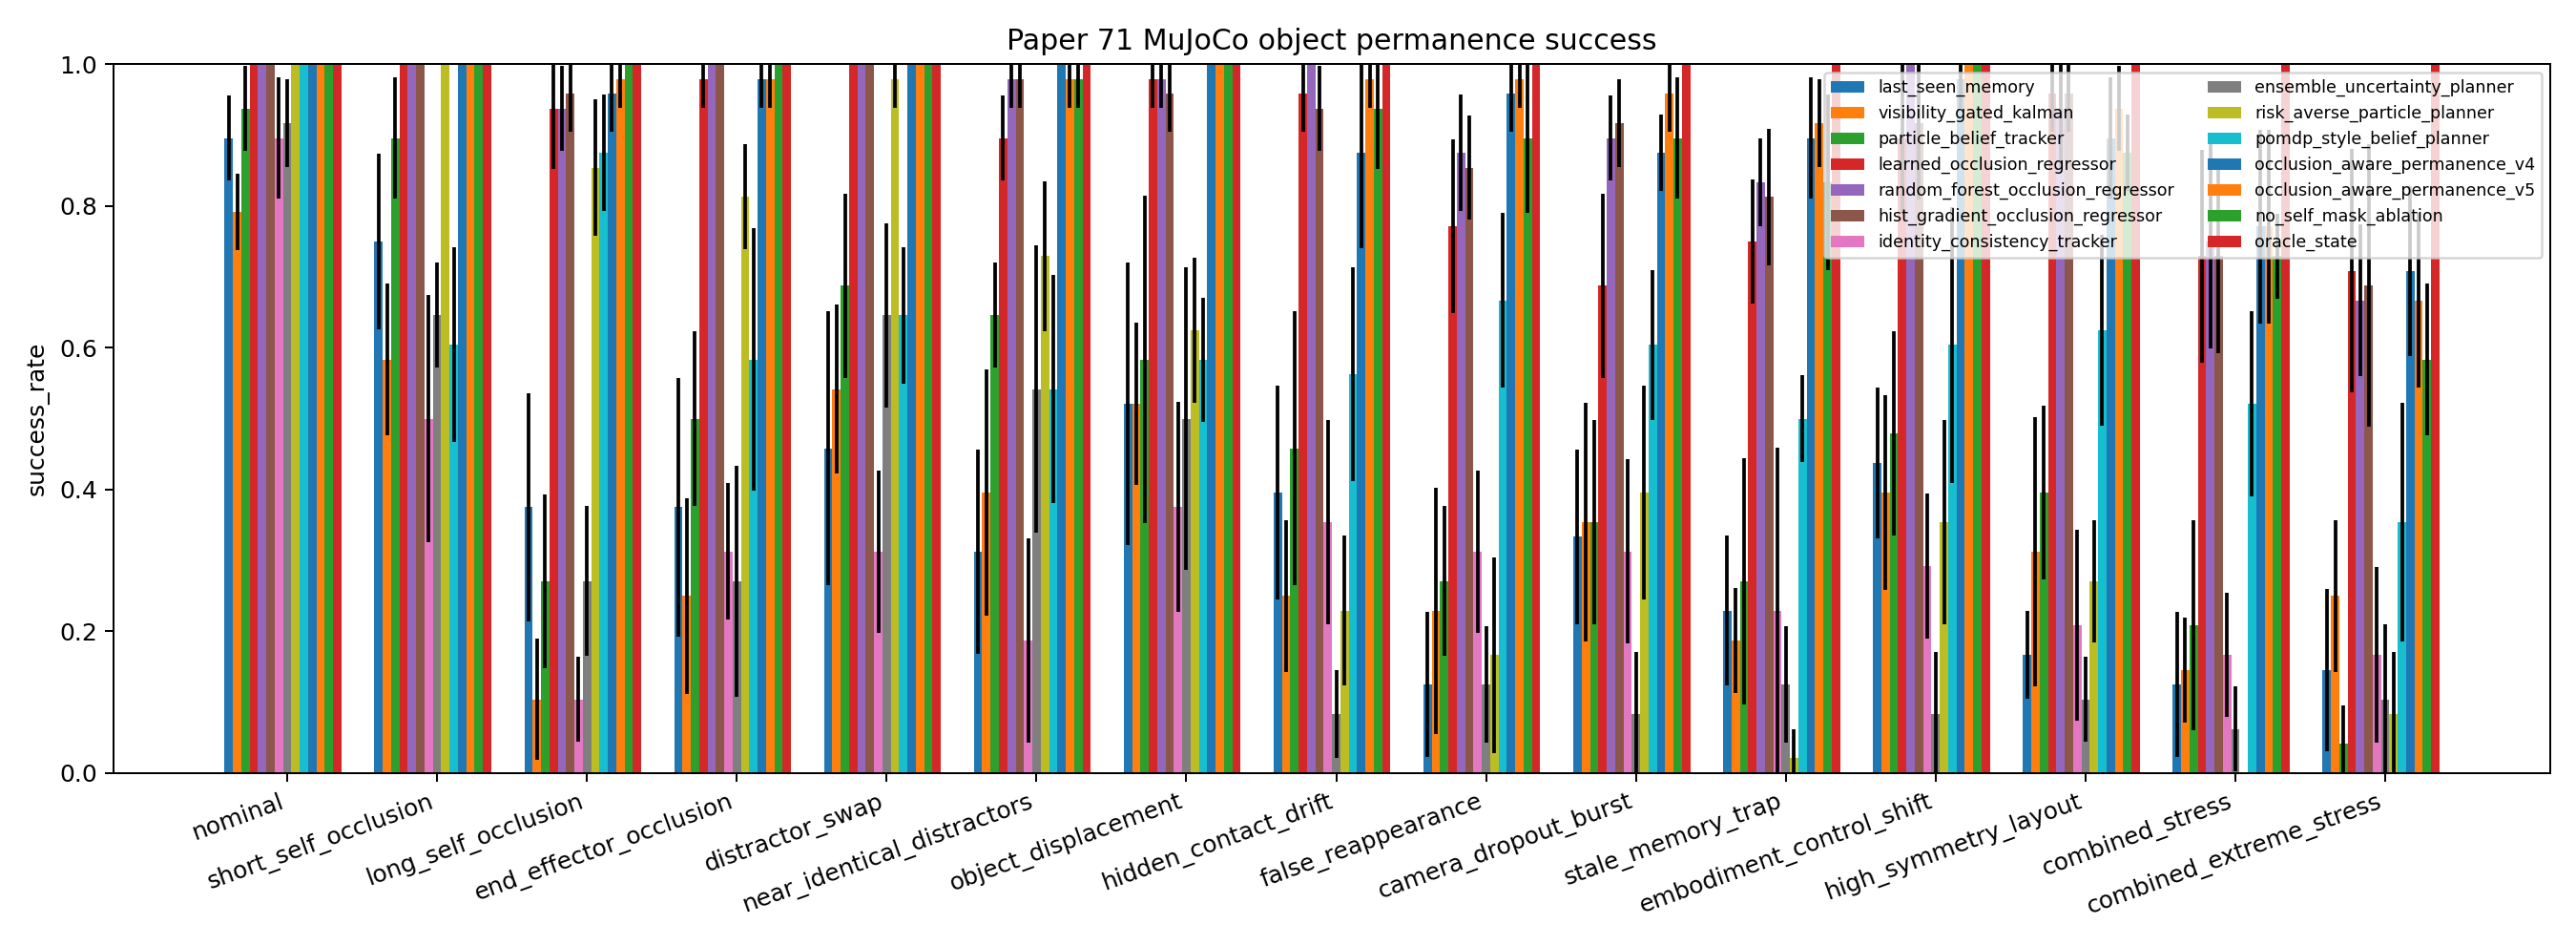
\includegraphics[width=\linewidth]{../figures/self_occlusion_success_by_split.png}
\caption{Success by split across all main methods. Strong learned and v4 replay baselines remain uncomfortable competitors.}
\label{fig:success}
\end{figure}

\begin{figure}[t]
\centering
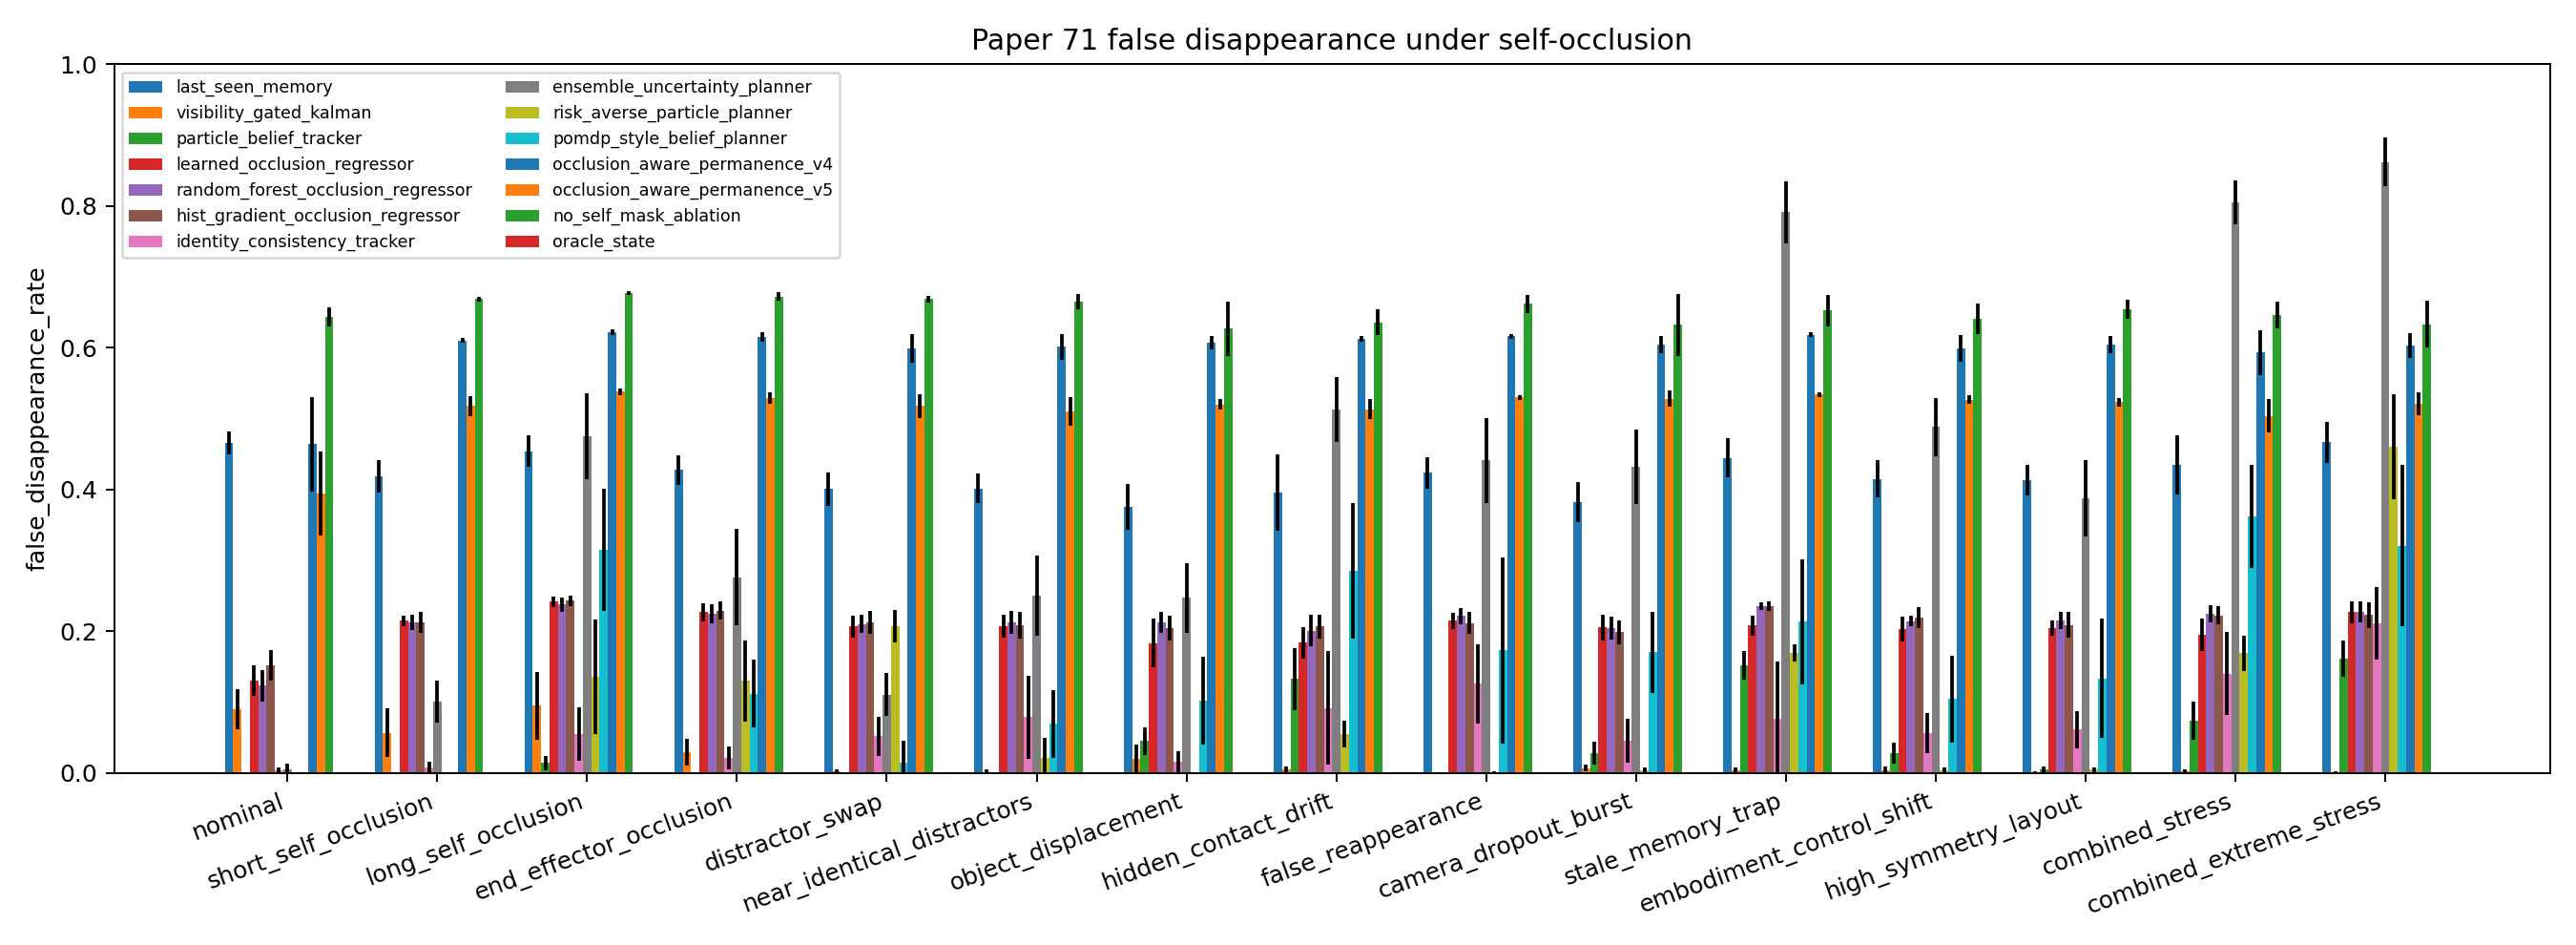
\includegraphics[width=\linewidth]{../figures/self_occlusion_false_disappearance.png}
\caption{False disappearance by split. This is a safety-relevant failure mode, not just a tracking diagnostic.}
\label{fig:false-disappearance}
\end{figure}

\begin{figure}[t]
\centering
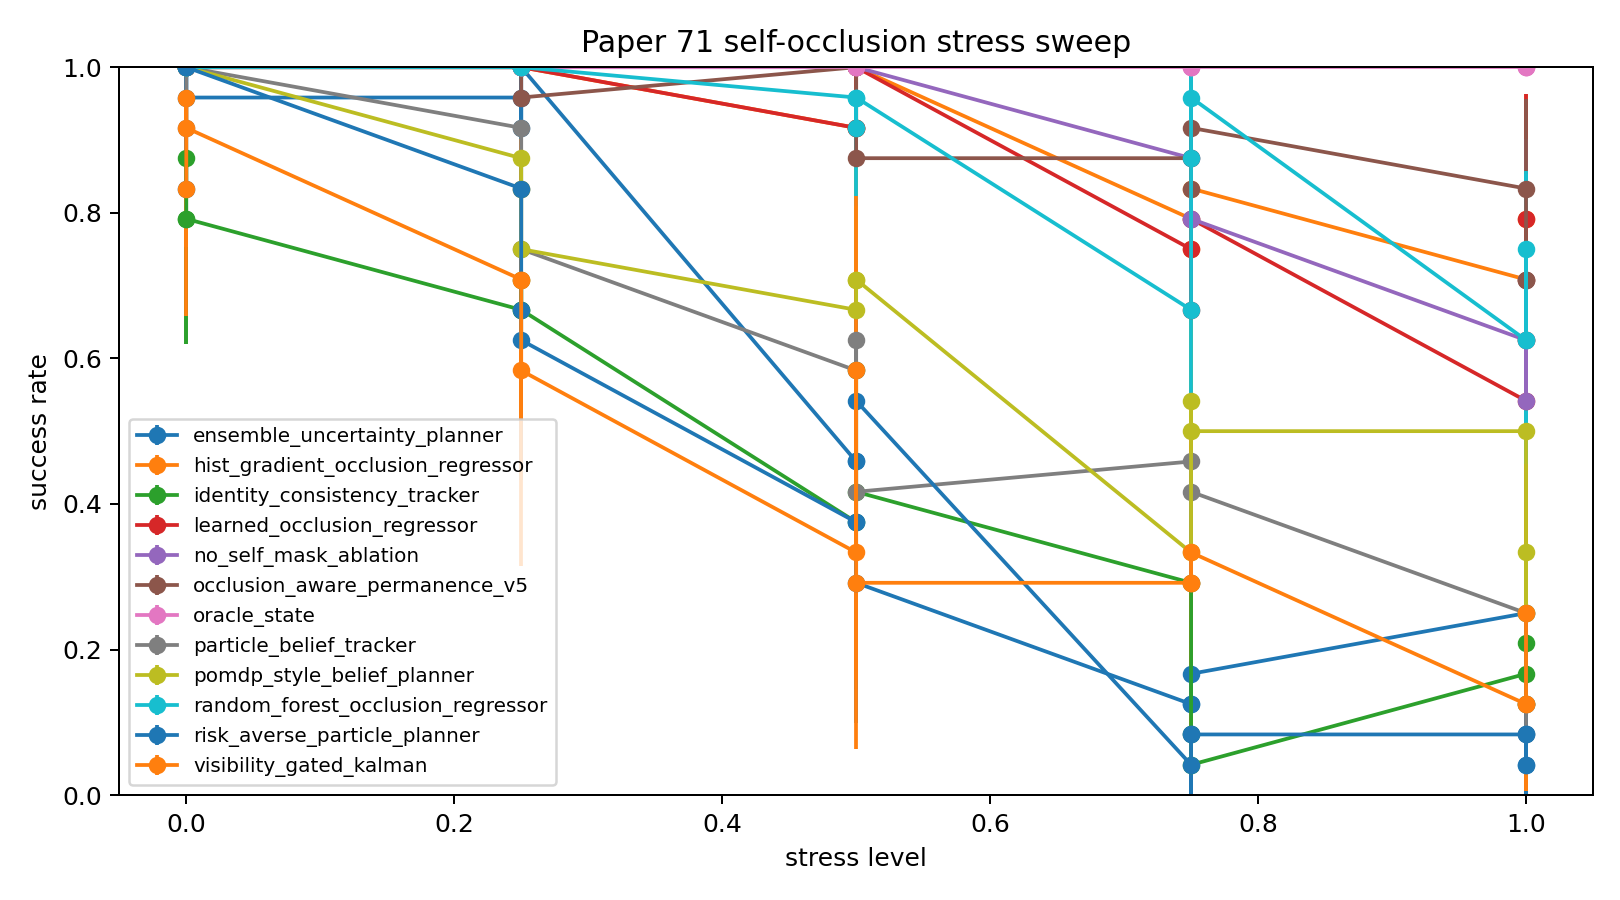
\includegraphics[width=0.92\linewidth]{../figures/self_occlusion_stress_sweep.png}
\caption{Stress sweep success. The frozen maximum-stress gate is applied before seeing the final result.}
\label{fig:stress}
\end{figure}

\section{Ablations}
\begin{table}[t]
\centering
\caption{Occlusion-aware permanence v5 ablations aggregated over frozen ablation splits.}
\label{tab:ablation}
\small
\begin{tabular}{lrrrrr}
\toprule
Ablation & Success & False disp. & Wrong obj. & Id switch & Occ. err. \\
\midrule
ablate no reacquisition guard & 0.906 & 0.524 & 0.000 & 0.040 & 0.049 \\
ablate no false detection rejection & 0.891 & 0.529 & 0.000 & 0.063 & 0.051 \\
ablate no tail risk objective & 0.891 & 0.521 & 0.008 & 0.033 & 0.052 \\
ablate no uncertainty inflation & 0.867 & 0.000 & 0.000 & 0.052 & 0.050 \\
occlusion full v5 & 0.867 & 0.528 & 0.000 & 0.026 & 0.052 \\
ablate no branch belief & 0.852 & 0.523 & 0.000 & 0.072 & 0.052 \\
ablate no distractor filter & 0.852 & 0.529 & 0.000 & 0.082 & 0.053 \\
occlusion aware permanence v4 & 0.844 & 0.616 & 0.000 & 0.018 & 0.051 \\
ablate no identity filter & 0.820 & 0.614 & 0.000 & 0.067 & 0.051 \\
learned only branch & 0.812 & 0.228 & 0.000 & 0.040 & 0.057 \\
ablate no self mask & 0.805 & 0.661 & 0.000 & 0.057 & 0.067 \\
ablate no contact update & 0.773 & 0.526 & 0.000 & 0.031 & 0.057 \\
\bottomrule
\end{tabular}
\end{table}


The ablation table is the most direct mechanism test.
Full v5 is not cleanly separated from removals of branch belief, distractor filtering, false-detection rejection, reacquisition guard, tail-risk objective, or uncertainty inflation.
Some removals improve success or remove false disappearance without enough compensating harm.
That means the branch story is not established by the benchmark.

\begin{figure}[t]
\centering
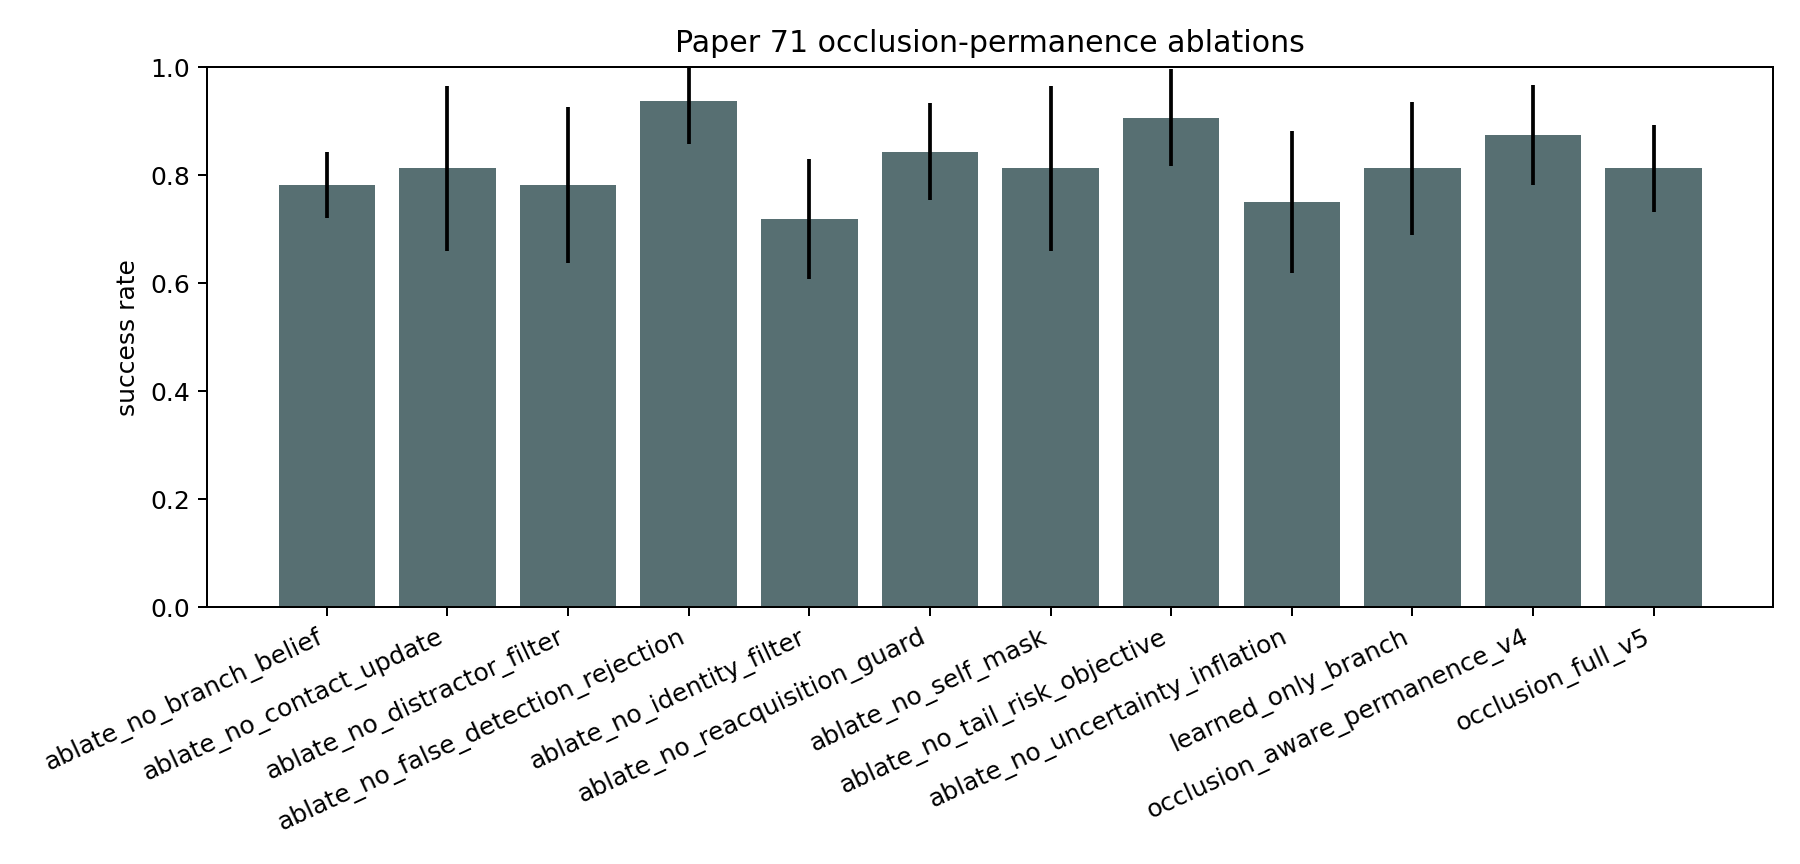
\includegraphics[width=0.84\linewidth]{../figures/self_occlusion_ablation_success.png}
\caption{Ablation success over frozen hard ablation splits. The method fails the component-necessity gate.}
\label{fig:ablation}
\end{figure}

\section{Negative Cases}
\begin{table}[t]
\centering
\caption{Representative frozen negative cases for occlusion-aware permanence v5.}
\label{tab:negative-cases}
\scriptsize
\begin{tabular}{llllrrrr}
\toprule
Case & Split & Seed & Ep. & Success & Wrong & Occ. err. & Id switch \\
\midrule
0 & combined extreme stress & 2 & 4 & 0 & 0 & 0.132 & 0.032 \\
1 & combined extreme stress & 0 & 3 & 0 & 0 & 0.123 & 0.031 \\
2 & combined extreme stress & 4 & 4 & 0 & 1 & 0.114 & 0.026 \\
3 & combined stress & 5 & 3 & 0 & 0 & 0.114 & 0.000 \\
4 & combined stress & 4 & 0 & 0 & 0 & 0.112 & 0.000 \\
5 & combined extreme stress & 6 & 0 & 0 & 0 & 0.110 & 0.000 \\
6 & combined stress & 2 & 1 & 0 & 0 & 0.108 & 0.000 \\
7 & combined extreme stress & 0 & 2 & 0 & 0 & 0.105 & 0.000 \\
8 & combined stress & 0 & 4 & 0 & 0 & 0.103 & 0.000 \\
9 & combined stress & 3 & 3 & 0 & 0 & 0.103 & 0.000 \\
10 & combined extreme stress & 4 & 5 & 0 & 0 & 0.102 & 0.676 \\
11 & combined extreme stress & 2 & 3 & 0 & 0 & 0.101 & 0.853 \\
\bottomrule
\end{tabular}
\end{table}


The negative cases are not outliers to hide.
They expose the scientific failure modes: hidden displacement can exceed the branch update; false reappearance can compete with target permanence; prolonged stale memory can remain confident in the wrong place; and identity switches can occur before the diagnostic motion recovers visibility.
These are precisely the cases a submission would need to solve.

\section{Theory: When Self-Occlusion Geometry Helps}
\paragraph{Proposition 1: self-mask informativeness.}
Let $Y_t$ be the camera observation and $M_t$ the known robot self-occlusion event.
If $P(Y_t=\emptyset\mid M_t=1,o_t=o)$ differs across object hypotheses only through the known robot geometry, then a belief update that conditions on $M_t$ can reduce posterior entropy relative to a missing-at-random filter.
This supports the intuition behind v5.

\paragraph{Proposition 2: learned-baseline non-identifiability.}
If the feature vector supplied to a learned baseline contains the same last-visible state, tool state, occlusion age, noise level, false-detection flag, and drift proxy used by the explicit branch mechanism, then a sufficiently flexible regressor can approximate the branch posterior mean on the benchmark distribution.
In that case, a local benchmark cannot identify the explicit branch object as necessary unless v5 beats the learned baseline under held-out stress and safety gates.
This is the failure observed here.

\paragraph{Proposition 3: ablation necessity.}
Let $M$ be full v5 and $M_{-j}$ remove component $j$.
If $S(M)-S(M_{-j})<\delta$ and $M_{-j}$ is not worse on false disappearance, wrong-object contact, identity switch, or calibration, then component $j$ is not locally supported.
The frozen ablation table violates this condition for several components.

\section{Related Work}
This paper sits between probabilistic tracking, partial-observability planning, and object-centric robot world models.
Kalman and particle filters remain strong baselines for occluded state estimation \citep{kalman1960new,gordon1993novel,thrun2005probabilistic}.
Robot manipulation under object uncertainty motivates belief-space and POMDP-style baselines \citep{pajarinen2023pomdp}.
Object-centric and scene-graph systems provide broader context for maintaining persistent object state in manipulation and navigation \citep{min2025asimo,loo2025open,honerkamp2024language,ren2024object,liu2026oawam,daniel2026latent}.
Visuo-haptic and keypoint approaches show that occluded object state can also be recovered through learned or multimodal representation \citep{rustler2023shape,hartz2022keypoints}.
This work does not beat those families; it creates a controlled negative audit of one explicit self-occlusion mechanism.

\section{Decision}
The frozen terminal reason is:
\begin{quote}\small\raggedright
\PaperReason{}\par
\end{quote}
The correct decision is \textbf{\PaperDecision{}}.
This is not a writing failure.
It is a scientific result: explicit self-occlusion permanence is a plausible mechanism, but this benchmark does not prove it is necessary over strong learned, v4 replay, and ablated baselines.

\clearpage
\appendix
\section{Frozen Protocol}
The plan-first document is \path{docs/paper71_expanded_submission_plan_20260621.md}.
The development log is \path{docs/paper71_development_log_20260621.md}.
The protocol freeze is \path{docs/paper71_protocol_freeze_20260621.md}.
No split, method, metric, or gate was changed after the protocol freeze.

\section{Full Split-Method Metrics}
\begingroup
\scriptsize
\setlength{\tabcolsep}{0.8pt}
\renewcommand{\arraystretch}{0.88}
\setlength{\LTleft}{0pt}
\setlength{\LTright}{0pt}
\begin{longtable}{@{}>{\raggedright\arraybackslash}p{0.20\linewidth} >{\raggedright\arraybackslash}p{0.18\linewidth} >{\raggedleft\arraybackslash}p{0.055\linewidth} >{\raggedleft\arraybackslash}p{0.060\linewidth} >{\raggedleft\arraybackslash}p{0.055\linewidth} >{\raggedleft\arraybackslash}p{0.045\linewidth} >{\raggedleft\arraybackslash}p{0.055\linewidth}@{}}
\caption{Full split-method metrics.}\label{tab:full-metrics}\\
\toprule
Method & Split & Succ. & False & Wrong & ID & Err. \\
\midrule
\endfirsthead
\toprule
Method & Split & Succ. & False & Wrong & ID & Err. \\
\midrule
\endhead
ensemble uncertainty planner & camera dropout burst & 0.083 & 0.432 & 0.000 & 0.112 & 0.136 \\
ensemble uncertainty planner & combined extreme stress & 0.104 & 0.862 & 0.104 & 0.308 & 0.354 \\
ensemble uncertainty planner & combined stress & 0.062 & 0.805 & 0.000 & 0.237 & 0.278 \\
ensemble uncertainty planner & distractor swap & 0.646 & 0.111 & 0.000 & 0.103 & 0.092 \\
ensemble uncertainty planner & embodiment control shift & 0.083 & 0.489 & 0.000 & 0.099 & 0.118 \\
ensemble uncertainty planner & end effector occlusion & 0.271 & 0.276 & 0.000 & 0.082 & 0.156 \\
ensemble uncertainty planner & false reappearance & 0.125 & 0.441 & 0.000 & 0.124 & 0.152 \\
ensemble uncertainty planner & hidden contact drift & 0.083 & 0.513 & 0.000 & 0.107 & 0.125 \\
ensemble uncertainty planner & high symmetry layout & 0.104 & 0.387 & 0.000 & 0.088 & 0.116 \\
ensemble uncertainty planner & long self occlusion & 0.271 & 0.475 & 0.000 & 0.186 & 0.227 \\
ensemble uncertainty planner & near identical distractors & 0.542 & 0.250 & 0.000 & 0.118 & 0.118 \\
ensemble uncertainty planner & nominal & 0.917 & 0.006 & 0.000 & 0.042 & 0.105 \\
ensemble uncertainty planner & object displacement & 0.500 & 0.247 & 0.000 & 0.044 & 0.080 \\
ensemble uncertainty planner & short self occlusion & 0.646 & 0.101 & 0.000 & 0.112 & 0.135 \\
ensemble uncertainty planner & stale memory trap & 0.125 & 0.791 & 0.000 & 0.187 & 0.230 \\
hist gradient occlusion regressor & camera dropout burst & 0.917 & 0.199 & 0.000 & 0.237 & 0.064 \\
hist gradient occlusion regressor & combined extreme stress & 0.688 & 0.223 & 0.000 & 0.352 & 0.079 \\
hist gradient occlusion regressor & combined stress & 0.729 & 0.222 & 0.000 & 0.289 & 0.068 \\
hist gradient occlusion regressor & distractor swap & 1.000 & 0.213 & 0.000 & 0.338 & 0.048 \\
hist gradient occlusion regressor & embodiment control shift & 0.917 & 0.219 & 0.000 & 0.301 & 0.052 \\
hist gradient occlusion regressor & end effector occlusion & 1.000 & 0.229 & 0.000 & 0.171 & 0.040 \\
hist gradient occlusion regressor & false reappearance & 0.854 & 0.212 & 0.000 & 0.305 & 0.065 \\
hist gradient occlusion regressor & hidden contact drift & 0.938 & 0.207 & 0.000 & 0.221 & 0.055 \\
hist gradient occlusion regressor & high symmetry layout & 0.958 & 0.209 & 0.000 & 0.212 & 0.053 \\
hist gradient occlusion regressor & long self occlusion & 0.958 & 0.243 & 0.000 & 0.118 & 0.047 \\
hist gradient occlusion regressor & near identical distractors & 0.979 & 0.209 & 0.000 & 0.197 & 0.052 \\
hist gradient occlusion regressor & nominal & 1.000 & 0.152 & 0.000 & 0.087 & 0.020 \\
hist gradient occlusion regressor & object displacement & 0.958 & 0.205 & 0.000 & 0.163 & 0.046 \\
hist gradient occlusion regressor & short self occlusion & 1.000 & 0.213 & 0.000 & 0.045 & 0.036 \\
hist gradient occlusion regressor & stale memory trap & 0.812 & 0.236 & 0.000 & 0.223 & 0.060 \\
identity consistency tracker & camera dropout burst & 0.312 & 0.046 & 0.000 & 0.404 & 0.235 \\
identity consistency tracker & combined extreme stress & 0.167 & 0.212 & 0.000 & 0.549 & 0.212 \\
identity consistency tracker & combined stress & 0.167 & 0.140 & 0.000 & 0.557 & 0.222 \\
identity consistency tracker & distractor swap & 0.312 & 0.052 & 0.000 & 0.617 & 0.181 \\
identity consistency tracker & embodiment control shift & 0.292 & 0.056 & 0.000 & 0.561 & 0.208 \\
identity consistency tracker & end effector occlusion & 0.312 & 0.021 & 0.000 & 0.381 & 0.209 \\
identity consistency tracker & false reappearance & 0.312 & 0.126 & 0.000 & 0.647 & 0.191 \\
identity consistency tracker & hidden contact drift & 0.354 & 0.092 & 0.000 & 0.485 & 0.226 \\
identity consistency tracker & high symmetry layout & 0.208 & 0.061 & 0.000 & 0.603 & 0.192 \\
identity consistency tracker & long self occlusion & 0.104 & 0.055 & 0.000 & 0.250 & 0.235 \\
identity consistency tracker & near identical distractors & 0.188 & 0.079 & 0.000 & 0.623 & 0.185 \\
identity consistency tracker & nominal & 0.896 & 0.003 & 0.000 & 0.097 & 0.093 \\
identity consistency tracker & object displacement & 0.375 & 0.016 & 0.000 & 0.382 & 0.229 \\
identity consistency tracker & short self occlusion & 0.500 & 0.008 & 0.000 & 0.231 & 0.173 \\
identity consistency tracker & stale memory trap & 0.229 & 0.077 & 0.000 & 0.460 & 0.233 \\
last seen memory & camera dropout burst & 0.333 & 0.382 & 0.000 & 0.927 & 0.180 \\
last seen memory & combined extreme stress & 0.146 & 0.467 & 0.125 & 0.830 & 0.166 \\
last seen memory & combined stress & 0.125 & 0.435 & 0.000 & 0.861 & 0.163 \\
last seen memory & distractor swap & 0.458 & 0.401 & 0.000 & 0.950 & 0.123 \\
last seen memory & embodiment control shift & 0.438 & 0.415 & 0.000 & 0.950 & 0.137 \\
last seen memory & end effector occlusion & 0.375 & 0.427 & 0.000 & 0.968 & 0.131 \\
last seen memory & false reappearance & 0.125 & 0.423 & 0.000 & 0.944 & 0.157 \\
last seen memory & hidden contact drift & 0.396 & 0.396 & 0.000 & 0.957 & 0.162 \\
last seen memory & high symmetry layout & 0.167 & 0.413 & 0.000 & 0.929 & 0.142 \\
last seen memory & long self occlusion & 0.375 & 0.454 & 0.000 & 0.973 & 0.141 \\
last seen memory & near identical distractors & 0.312 & 0.401 & 0.000 & 0.932 & 0.133 \\
last seen memory & nominal & 0.896 & 0.465 & 0.000 & 0.667 & 0.043 \\
last seen memory & object displacement & 0.521 & 0.376 & 0.000 & 0.972 & 0.133 \\
last seen memory & short self occlusion & 0.750 & 0.419 & 0.000 & 1.000 & 0.082 \\
last seen memory & stale memory trap & 0.229 & 0.445 & 0.000 & 0.921 & 0.168 \\
learned occlusion regressor & camera dropout burst & 0.688 & 0.205 & 0.000 & 0.590 & 0.076 \\
learned occlusion regressor & combined extreme stress & 0.708 & 0.227 & 0.000 & 0.531 & 0.086 \\
learned occlusion regressor & combined stress & 0.729 & 0.195 & 0.000 & 0.557 & 0.078 \\
learned occlusion regressor & distractor swap & 1.000 & 0.207 & 0.000 & 0.509 & 0.050 \\
learned occlusion regressor & embodiment control shift & 0.896 & 0.203 & 0.000 & 0.612 & 0.058 \\
learned occlusion regressor & end effector occlusion & 0.979 & 0.227 & 0.000 & 0.656 & 0.045 \\
learned occlusion regressor & false reappearance & 0.771 & 0.215 & 0.000 & 0.595 & 0.070 \\
learned occlusion regressor & hidden contact drift & 0.958 & 0.184 & 0.000 & 0.658 & 0.061 \\
learned occlusion regressor & high symmetry layout & 0.958 & 0.205 & 0.000 & 0.535 & 0.063 \\
learned occlusion regressor & long self occlusion & 0.938 & 0.242 & 0.000 & 0.515 & 0.047 \\
learned occlusion regressor & near identical distractors & 0.896 & 0.208 & 0.000 & 0.518 & 0.058 \\
learned occlusion regressor & nominal & 1.000 & 0.131 & 0.000 & 0.413 & 0.020 \\
learned occlusion regressor & object displacement & 0.979 & 0.184 & 0.000 & 0.611 & 0.054 \\
learned occlusion regressor & short self occlusion & 1.000 & 0.215 & 0.000 & 0.617 & 0.036 \\
learned occlusion regressor & stale memory trap & 0.750 & 0.208 & 0.000 & 0.630 & 0.073 \\
no self mask ablation & camera dropout burst & 0.896 & 0.632 & 0.000 & 0.025 & 0.055 \\
no self mask ablation & combined extreme stress & 0.583 & 0.633 & 0.000 & 0.076 & 0.086 \\
no self mask ablation & combined stress & 0.729 & 0.646 & 0.000 & 0.069 & 0.070 \\
no self mask ablation & distractor swap & 1.000 & 0.669 & 0.000 & 0.007 & 0.035 \\
no self mask ablation & embodiment control shift & 1.000 & 0.641 & 0.000 & 0.006 & 0.048 \\
no self mask ablation & end effector occlusion & 1.000 & 0.672 & 0.000 & 0.006 & 0.032 \\
no self mask ablation & false reappearance & 0.896 & 0.662 & 0.000 & 0.010 & 0.050 \\
no self mask ablation & hidden contact drift & 0.938 & 0.636 & 0.000 & 0.031 & 0.057 \\
no self mask ablation & high symmetry layout & 0.875 & 0.654 & 0.000 & 0.056 & 0.050 \\
no self mask ablation & long self occlusion & 1.000 & 0.677 & 0.000 & 0.000 & 0.040 \\
no self mask ablation & near identical distractors & 0.979 & 0.665 & 0.000 & 0.035 & 0.041 \\
no self mask ablation & nominal & 1.000 & 0.643 & 0.000 & 0.000 & 0.015 \\
no self mask ablation & object displacement & 1.000 & 0.627 & 0.000 & 0.008 & 0.045 \\
no self mask ablation & short self occlusion & 1.000 & 0.668 & 0.000 & 0.003 & 0.026 \\
no self mask ablation & stale memory trap & 0.833 & 0.652 & 0.000 & 0.050 & 0.069 \\
occlusion aware permanence v4 & camera dropout burst & 0.875 & 0.604 & 0.000 & 0.006 & 0.051 \\
occlusion aware permanence v4 & combined extreme stress & 0.708 & 0.604 & 0.000 & 0.040 & 0.071 \\
occlusion aware permanence v4 & combined stress & 0.771 & 0.593 & 0.000 & 0.055 & 0.059 \\
occlusion aware permanence v4 & distractor swap & 1.000 & 0.599 & 0.000 & 0.002 & 0.038 \\
occlusion aware permanence v4 & embodiment control shift & 0.979 & 0.599 & 0.000 & 0.041 & 0.043 \\
occlusion aware permanence v4 & end effector occlusion & 0.979 & 0.615 & 0.000 & 0.003 & 0.035 \\
occlusion aware permanence v4 & false reappearance & 0.958 & 0.616 & 0.000 & 0.023 & 0.044 \\
occlusion aware permanence v4 & hidden contact drift & 0.875 & 0.612 & 0.000 & 0.035 & 0.043 \\
occlusion aware permanence v4 & high symmetry layout & 0.896 & 0.604 & 0.000 & 0.003 & 0.042 \\
occlusion aware permanence v4 & long self occlusion & 0.958 & 0.622 & 0.000 & 0.000 & 0.038 \\
occlusion aware permanence v4 & near identical distractors & 1.000 & 0.601 & 0.000 & 0.031 & 0.039 \\
occlusion aware permanence v4 & nominal & 1.000 & 0.464 & 0.000 & 0.000 & 0.022 \\
occlusion aware permanence v4 & object displacement & 1.000 & 0.607 & 0.000 & 0.006 & 0.040 \\
occlusion aware permanence v4 & short self occlusion & 1.000 & 0.610 & 0.000 & 0.000 & 0.031 \\
occlusion aware permanence v4 & stale memory trap & 0.896 & 0.618 & 0.000 & 0.033 & 0.044 \\
occlusion aware permanence v5 & camera dropout burst & 0.958 & 0.528 & 0.000 & 0.021 & 0.040 \\
occlusion aware permanence v5 & combined extreme stress & 0.667 & 0.521 & 0.021 & 0.088 & 0.064 \\
occlusion aware permanence v5 & combined stress & 0.771 & 0.504 & 0.000 & 0.056 & 0.062 \\
occlusion aware permanence v5 & distractor swap & 1.000 & 0.518 & 0.000 & 0.005 & 0.034 \\
occlusion aware permanence v5 & embodiment control shift & 1.000 & 0.527 & 0.000 & 0.000 & 0.038 \\
occlusion aware permanence v5 & end effector occlusion & 0.979 & 0.529 & 0.000 & 0.000 & 0.036 \\
occlusion aware permanence v5 & false reappearance & 0.979 & 0.530 & 0.000 & 0.004 & 0.043 \\
occlusion aware permanence v5 & hidden contact drift & 0.979 & 0.513 & 0.000 & 0.000 & 0.038 \\
occlusion aware permanence v5 & high symmetry layout & 0.938 & 0.523 & 0.000 & 0.021 & 0.044 \\
occlusion aware permanence v5 & long self occlusion & 0.979 & 0.538 & 0.000 & 0.000 & 0.038 \\
occlusion aware permanence v5 & near identical distractors & 0.979 & 0.510 & 0.000 & 0.003 & 0.039 \\
occlusion aware permanence v5 & nominal & 1.000 & 0.394 & 0.000 & 0.000 & 0.019 \\
occlusion aware permanence v5 & object displacement & 1.000 & 0.520 & 0.000 & 0.000 & 0.035 \\
occlusion aware permanence v5 & short self occlusion & 1.000 & 0.518 & 0.000 & 0.000 & 0.031 \\
occlusion aware permanence v5 & stale memory trap & 0.917 & 0.534 & 0.000 & 0.027 & 0.046 \\
oracle state & camera dropout burst & 1.000 & 0.000 & 0.000 & 0.000 & 0.000 \\
oracle state & combined extreme stress & 1.000 & 0.000 & 0.000 & 0.000 & 0.001 \\
oracle state & combined stress & 1.000 & 0.000 & 0.000 & 0.000 & 0.000 \\
oracle state & distractor swap & 1.000 & 0.000 & 0.000 & 0.000 & 0.000 \\
oracle state & embodiment control shift & 1.000 & 0.000 & 0.000 & 0.000 & 0.000 \\
oracle state & end effector occlusion & 1.000 & 0.000 & 0.000 & 0.000 & 0.000 \\
oracle state & false reappearance & 1.000 & 0.000 & 0.000 & 0.000 & 0.000 \\
oracle state & hidden contact drift & 1.000 & 0.000 & 0.000 & 0.000 & 0.000 \\
oracle state & high symmetry layout & 1.000 & 0.000 & 0.000 & 0.000 & 0.000 \\
oracle state & long self occlusion & 1.000 & 0.000 & 0.000 & 0.000 & 0.000 \\
oracle state & near identical distractors & 1.000 & 0.000 & 0.000 & 0.000 & 0.000 \\
oracle state & nominal & 1.000 & 0.000 & 0.000 & 0.000 & 0.000 \\
oracle state & object displacement & 1.000 & 0.000 & 0.000 & 0.000 & 0.000 \\
oracle state & short self occlusion & 1.000 & 0.000 & 0.000 & 0.000 & 0.000 \\
oracle state & stale memory trap & 1.000 & 0.000 & 0.000 & 0.000 & 0.000 \\
particle belief tracker & camera dropout burst & 0.354 & 0.028 & 0.000 & 0.609 & 0.127 \\
particle belief tracker & combined extreme stress & 0.042 & 0.161 & 0.000 & 0.751 & 0.137 \\
particle belief tracker & combined stress & 0.208 & 0.074 & 0.000 & 0.721 & 0.128 \\
particle belief tracker & distractor swap & 0.688 & 0.000 & 0.000 & 0.534 & 0.077 \\
particle belief tracker & embodiment control shift & 0.479 & 0.028 & 0.000 & 0.725 & 0.114 \\
particle belief tracker & end effector occlusion & 0.500 & 0.000 & 0.000 & 0.570 & 0.089 \\
particle belief tracker & false reappearance & 0.271 & 0.000 & 0.000 & 0.720 & 0.122 \\
particle belief tracker & hidden contact drift & 0.458 & 0.133 & 0.000 & 0.756 & 0.129 \\
particle belief tracker & high symmetry layout & 0.396 & 0.005 & 0.000 & 0.714 & 0.113 \\
particle belief tracker & long self occlusion & 0.271 & 0.014 & 0.000 & 0.613 & 0.102 \\
particle belief tracker & near identical distractors & 0.646 & 0.000 & 0.000 & 0.580 & 0.086 \\
particle belief tracker & nominal & 0.938 & 0.000 & 0.000 & 0.149 & 0.021 \\
particle belief tracker & object displacement & 0.583 & 0.045 & 0.000 & 0.590 & 0.099 \\
particle belief tracker & short self occlusion & 0.896 & 0.000 & 0.000 & 0.282 & 0.048 \\
particle belief tracker & stale memory trap & 0.271 & 0.152 & 0.000 & 0.785 & 0.142 \\
pomdp style belief planner & camera dropout burst & 0.604 & 0.170 & 0.000 & 0.050 & 0.071 \\
pomdp style belief planner & combined extreme stress & 0.354 & 0.321 & 0.000 & 0.089 & 0.107 \\
pomdp style belief planner & combined stress & 0.521 & 0.362 & 0.000 & 0.079 & 0.086 \\
pomdp style belief planner & distractor swap & 0.646 & 0.015 & 0.000 & 0.032 & 0.047 \\
pomdp style belief planner & embodiment control shift & 0.604 & 0.104 & 0.000 & 0.010 & 0.068 \\
pomdp style belief planner & end effector occlusion & 0.583 & 0.112 & 0.000 & 0.023 & 0.046 \\
pomdp style belief planner & false reappearance & 0.667 & 0.173 & 0.000 & 0.044 & 0.067 \\
pomdp style belief planner & hidden contact drift & 0.562 & 0.285 & 0.000 & 0.062 & 0.083 \\
pomdp style belief planner & high symmetry layout & 0.625 & 0.134 & 0.000 & 0.040 & 0.067 \\
pomdp style belief planner & long self occlusion & 0.875 & 0.315 & 0.000 & 0.000 & 0.043 \\
pomdp style belief planner & near identical distractors & 0.542 & 0.070 & 0.000 & 0.018 & 0.056 \\
pomdp style belief planner & nominal & 1.000 & 0.000 & 0.000 & 0.000 & 0.023 \\
pomdp style belief planner & object displacement & 0.583 & 0.103 & 0.000 & 0.013 & 0.070 \\
pomdp style belief planner & short self occlusion & 0.604 & 0.000 & 0.000 & 0.007 & 0.040 \\
pomdp style belief planner & stale memory trap & 0.500 & 0.214 & 0.000 & 0.057 & 0.083 \\
random forest occlusion regressor & camera dropout burst & 0.896 & 0.204 & 0.000 & 0.079 & 0.054 \\
random forest occlusion regressor & combined extreme stress & 0.667 & 0.228 & 0.000 & 0.138 & 0.071 \\
random forest occlusion regressor & combined stress & 0.750 & 0.225 & 0.000 & 0.092 & 0.067 \\
random forest occlusion regressor & distractor swap & 1.000 & 0.210 & 0.000 & 0.055 & 0.043 \\
random forest occlusion regressor & embodiment control shift & 1.000 & 0.214 & 0.000 & 0.097 & 0.047 \\
random forest occlusion regressor & end effector occlusion & 1.000 & 0.224 & 0.000 & 0.047 & 0.041 \\
random forest occlusion regressor & false reappearance & 0.875 & 0.222 & 0.000 & 0.127 & 0.055 \\
random forest occlusion regressor & hidden contact drift & 1.000 & 0.201 & 0.000 & 0.042 & 0.051 \\
random forest occlusion regressor & high symmetry layout & 0.938 & 0.215 & 0.000 & 0.086 & 0.051 \\
random forest occlusion regressor & long self occlusion & 0.938 & 0.238 & 0.000 & 0.084 & 0.047 \\
random forest occlusion regressor & near identical distractors & 0.979 & 0.213 & 0.000 & 0.086 & 0.048 \\
random forest occlusion regressor & nominal & 1.000 & 0.123 & 0.000 & 0.026 & 0.022 \\
random forest occlusion regressor & object displacement & 0.979 & 0.213 & 0.000 & 0.037 & 0.045 \\
random forest occlusion regressor & short self occlusion & 1.000 & 0.213 & 0.000 & 0.000 & 0.034 \\
random forest occlusion regressor & stale memory trap & 0.833 & 0.235 & 0.000 & 0.088 & 0.056 \\
risk averse particle planner & camera dropout burst & 0.396 & 0.004 & 0.000 & 0.001 & 0.034 \\
risk averse particle planner & combined extreme stress & 0.083 & 0.461 & 0.021 & 0.048 & 0.064 \\
risk averse particle planner & combined stress & 0.000 & 0.169 & 0.021 & 0.006 & 0.040 \\
risk averse particle planner & distractor swap & 0.979 & 0.207 & 0.000 & 0.000 & 0.025 \\
risk averse particle planner & embodiment control shift & 0.354 & 0.004 & 0.000 & 0.002 & 0.029 \\
risk averse particle planner & end effector occlusion & 0.812 & 0.130 & 0.000 & 0.000 & 0.024 \\
risk averse particle planner & false reappearance & 0.167 & 0.001 & 0.000 & 0.000 & 0.031 \\
risk averse particle planner & hidden contact drift & 0.229 & 0.055 & 0.000 & 0.000 & 0.032 \\
risk averse particle planner & high symmetry layout & 0.271 & 0.005 & 0.000 & 0.000 & 0.031 \\
risk averse particle planner & long self occlusion & 0.854 & 0.136 & 0.000 & 0.000 & 0.025 \\
risk averse particle planner & near identical distractors & 0.729 & 0.022 & 0.000 & 0.000 & 0.023 \\
risk averse particle planner & nominal & 1.000 & 0.000 & 0.000 & 0.000 & 0.012 \\
risk averse particle planner & object displacement & 0.625 & 0.000 & 0.000 & 0.000 & 0.025 \\
risk averse particle planner & short self occlusion & 1.000 & 0.000 & 0.000 & 0.000 & 0.019 \\
risk averse particle planner & stale memory trap & 0.021 & 0.170 & 0.000 & 0.000 & 0.033 \\
visibility gated kalman & camera dropout burst & 0.354 & 0.007 & 0.000 & 0.577 & 0.214 \\
visibility gated kalman & combined extreme stress & 0.250 & 0.001 & 0.000 & 0.679 & 0.182 \\
visibility gated kalman & combined stress & 0.146 & 0.002 & 0.000 & 0.647 & 0.192 \\
visibility gated kalman & distractor swap & 0.542 & 0.003 & 0.000 & 0.647 & 0.155 \\
visibility gated kalman & embodiment control shift & 0.396 & 0.005 & 0.000 & 0.606 & 0.182 \\
visibility gated kalman & end effector occlusion & 0.250 & 0.030 & 0.000 & 0.476 & 0.185 \\
visibility gated kalman & false reappearance & 0.229 & 0.000 & 0.000 & 0.704 & 0.181 \\
visibility gated kalman & hidden contact drift & 0.250 & 0.005 & 0.000 & 0.629 & 0.195 \\
visibility gated kalman & high symmetry layout & 0.312 & 0.001 & 0.000 & 0.678 & 0.175 \\
visibility gated kalman & long self occlusion & 0.104 & 0.095 & 0.000 & 0.545 & 0.205 \\
visibility gated kalman & near identical distractors & 0.396 & 0.002 & 0.000 & 0.665 & 0.167 \\
visibility gated kalman & nominal & 0.792 & 0.090 & 0.000 & 0.186 & 0.084 \\
visibility gated kalman & object displacement & 0.521 & 0.021 & 0.000 & 0.529 & 0.183 \\
visibility gated kalman & short self occlusion & 0.583 & 0.057 & 0.000 & 0.326 & 0.146 \\
visibility gated kalman & stale memory trap & 0.188 & 0.003 & 0.000 & 0.646 & 0.210 \\
\bottomrule
\end{longtable}
\endgroup


\section{Full Aggregate Metrics}
\begingroup
\scriptsize
\setlength{\tabcolsep}{0.8pt}
\renewcommand{\arraystretch}{0.88}
\setlength{\LTleft}{0pt}
\setlength{\LTright}{0pt}
\begin{longtable}{@{}>{\raggedright\arraybackslash}p{0.18\linewidth} >{\raggedright\arraybackslash}p{0.20\linewidth} >{\raggedleft\arraybackslash}p{0.055\linewidth} >{\raggedleft\arraybackslash}p{0.060\linewidth} >{\raggedleft\arraybackslash}p{0.055\linewidth} >{\raggedleft\arraybackslash}p{0.045\linewidth} >{\raggedleft\arraybackslash}p{0.055\linewidth}@{}}
\caption{Full aggregate metrics.}\label{tab:full-aggregate}\\
\toprule
Group & Method & Succ. & False & Wrong & ID & Err. \\
\midrule
\endfirsthead
\toprule
Group & Method & Succ. & False & Wrong & ID & Err. \\
\midrule
\endhead
all splits & ensemble uncertainty planner & 0.304 & 0.412 & 0.007 & 0.130 & 0.161 \\
all splits & hist gradient occlusion regressor & 0.914 & 0.213 & 0.000 & 0.217 & 0.052 \\
all splits & identity consistency tracker & 0.315 & 0.070 & 0.000 & 0.456 & 0.202 \\
all splits & last seen memory & 0.376 & 0.421 & 0.008 & 0.919 & 0.137 \\
all splits & learned occlusion regressor & 0.883 & 0.204 & 0.000 & 0.570 & 0.058 \\
all splits & no self mask ablation & 0.915 & 0.652 & 0.000 & 0.025 & 0.048 \\
all splits & occlusion aware permanence v4 & 0.926 & 0.598 & 0.000 & 0.019 & 0.043 \\
all splits & occlusion aware permanence v5 & 0.943 & 0.514 & 0.001 & 0.015 & 0.040 \\
all splits & oracle state & 1.000 & 0.000 & 0.000 & 0.000 & 0.000 \\
all splits & particle belief tracker & 0.467 & 0.043 & 0.000 & 0.607 & 0.102 \\
all splits & pomdp style belief planner & 0.618 & 0.159 & 0.000 & 0.035 & 0.064 \\
all splits & random forest occlusion regressor & 0.924 & 0.212 & 0.000 & 0.072 & 0.049 \\
all splits & risk averse particle planner & 0.501 & 0.091 & 0.003 & 0.004 & 0.030 \\
all splits & visibility gated kalman & 0.354 & 0.021 & 0.000 & 0.569 & 0.177 \\
hard splits & ensemble uncertainty planner & 0.196 & 0.497 & 0.009 & 0.141 & 0.174 \\
hard splits & hist gradient occlusion regressor & 0.892 & 0.218 & 0.000 & 0.233 & 0.057 \\
hard splits & identity consistency tracker & 0.252 & 0.082 & 0.000 & 0.492 & 0.215 \\
hard splits & last seen memory & 0.295 & 0.419 & 0.010 & 0.930 & 0.151 \\
hard splits & learned occlusion regressor & 0.854 & 0.208 & 0.000 & 0.584 & 0.064 \\
hard splits & no self mask ablation & 0.894 & 0.650 & 0.000 & 0.031 & 0.053 \\
hard splits & occlusion aware permanence v4 & 0.908 & 0.608 & 0.000 & 0.023 & 0.046 \\
hard splits & occlusion aware permanence v5 & 0.929 & 0.523 & 0.002 & 0.018 & 0.044 \\
hard splits & oracle state & 1.000 & 0.000 & 0.000 & 0.000 & 0.000 \\
hard splits & particle belief tracker & 0.373 & 0.053 & 0.000 & 0.678 & 0.116 \\
hard splits & pomdp style belief planner & 0.585 & 0.197 & 0.000 & 0.040 & 0.070 \\
hard splits & random forest occlusion regressor & 0.905 & 0.219 & 0.000 & 0.084 & 0.053 \\
hard splits & risk averse particle planner & 0.378 & 0.096 & 0.003 & 0.005 & 0.033 \\
hard splits & visibility gated kalman & 0.283 & 0.014 & 0.000 & 0.615 & 0.189 \\
combined and extreme & ensemble uncertainty planner & 0.083 & 0.834 & 0.052 & 0.272 & 0.316 \\
combined and extreme & hist gradient occlusion regressor & 0.708 & 0.223 & 0.000 & 0.321 & 0.074 \\
combined and extreme & identity consistency tracker & 0.167 & 0.176 & 0.000 & 0.553 & 0.217 \\
combined and extreme & last seen memory & 0.135 & 0.451 & 0.062 & 0.845 & 0.165 \\
combined and extreme & learned occlusion regressor & 0.719 & 0.211 & 0.000 & 0.544 & 0.082 \\
combined and extreme & no self mask ablation & 0.656 & 0.640 & 0.000 & 0.072 & 0.078 \\
combined and extreme & occlusion aware permanence v4 & 0.740 & 0.598 & 0.000 & 0.048 & 0.065 \\
combined and extreme & occlusion aware permanence v5 & 0.719 & 0.512 & 0.010 & 0.072 & 0.063 \\
combined and extreme & oracle state & 1.000 & 0.000 & 0.000 & 0.000 & 0.001 \\
combined and extreme & particle belief tracker & 0.125 & 0.118 & 0.000 & 0.736 & 0.133 \\
combined and extreme & pomdp style belief planner & 0.438 & 0.341 & 0.000 & 0.084 & 0.096 \\
combined and extreme & random forest occlusion regressor & 0.708 & 0.226 & 0.000 & 0.115 & 0.069 \\
combined and extreme & risk averse particle planner & 0.042 & 0.315 & 0.021 & 0.027 & 0.052 \\
combined and extreme & visibility gated kalman & 0.198 & 0.002 & 0.000 & 0.663 & 0.187 \\
identity hard & ensemble uncertainty planner & 0.354 & 0.297 & 0.000 & 0.108 & 0.119 \\
identity hard & hist gradient occlusion regressor & 0.948 & 0.210 & 0.000 & 0.263 & 0.055 \\
identity hard & identity consistency tracker & 0.255 & 0.080 & 0.000 & 0.622 & 0.187 \\
identity hard & last seen memory & 0.266 & 0.410 & 0.000 & 0.939 & 0.139 \\
identity hard & learned occlusion regressor & 0.906 & 0.208 & 0.000 & 0.539 & 0.060 \\
identity hard & no self mask ablation & 0.938 & 0.662 & 0.000 & 0.027 & 0.044 \\
identity hard & occlusion aware permanence v4 & 0.964 & 0.605 & 0.000 & 0.015 & 0.041 \\
identity hard & occlusion aware permanence v5 & 0.974 & 0.520 & 0.000 & 0.008 & 0.040 \\
identity hard & oracle state & 1.000 & 0.000 & 0.000 & 0.000 & 0.000 \\
identity hard & particle belief tracker & 0.500 & 0.001 & 0.000 & 0.637 & 0.099 \\
identity hard & pomdp style belief planner & 0.620 & 0.098 & 0.000 & 0.033 & 0.059 \\
identity hard & random forest occlusion regressor & 0.948 & 0.215 & 0.000 & 0.089 & 0.049 \\
identity hard & risk averse particle planner & 0.536 & 0.059 & 0.000 & 0.000 & 0.028 \\
identity hard & visibility gated kalman & 0.370 & 0.001 & 0.000 & 0.674 & 0.169 \\
\bottomrule
\end{longtable}
\endgroup


\section{All Seed Metrics}
\begingroup
\scriptsize
\setlength{\tabcolsep}{0.8pt}
\renewcommand{\arraystretch}{0.88}
\setlength{\LTleft}{0pt}
\setlength{\LTright}{0pt}
\begin{longtable}{@{}>{\raggedright\arraybackslash}p{0.17\linewidth} >{\raggedright\arraybackslash}p{0.15\linewidth} >{\raggedleft\arraybackslash}p{0.045\linewidth} >{\raggedleft\arraybackslash}p{0.055\linewidth} >{\raggedleft\arraybackslash}p{0.060\linewidth} >{\raggedleft\arraybackslash}p{0.055\linewidth} >{\raggedleft\arraybackslash}p{0.045\linewidth} >{\raggedleft\arraybackslash}p{0.055\linewidth}@{}}
\caption{All seed-level metrics.}\label{tab:all-seeds}\\
\toprule
Method & Split & Seed & Succ. & False & Wrong & ID & Err. \\
\midrule
\endfirsthead
\toprule
Method & Split & Seed & Succ. & False & Wrong & ID & Err. \\
\midrule
\endhead
ensemble uncertainty planner & camera dropout burst & 0 & 0.000 & 0.322 & 0.000 & 0.031 & 0.083 \\
ensemble uncertainty planner & camera dropout burst & 1 & 0.000 & 0.374 & 0.000 & 0.021 & 0.087 \\
ensemble uncertainty planner & camera dropout burst & 2 & 0.333 & 0.470 & 0.000 & 0.077 & 0.134 \\
ensemble uncertainty planner & camera dropout burst & 3 & 0.000 & 0.379 & 0.000 & 0.094 & 0.093 \\
ensemble uncertainty planner & camera dropout burst & 4 & 0.000 & 0.463 & 0.000 & 0.168 & 0.182 \\
ensemble uncertainty planner & camera dropout burst & 5 & 0.000 & 0.570 & 0.000 & 0.284 & 0.230 \\
ensemble uncertainty planner & camera dropout burst & 6 & 0.167 & 0.435 & 0.000 & 0.102 & 0.153 \\
ensemble uncertainty planner & camera dropout burst & 7 & 0.167 & 0.445 & 0.000 & 0.122 & 0.123 \\
ensemble uncertainty planner & combined extreme stress & 0 & 0.000 & 0.824 & 0.167 & 0.250 & 0.328 \\
ensemble uncertainty planner & combined extreme stress & 1 & 0.000 & 0.931 & 0.000 & 0.398 & 0.465 \\
ensemble uncertainty planner & combined extreme stress & 2 & 0.167 & 0.871 & 0.000 & 0.319 & 0.381 \\
ensemble uncertainty planner & combined extreme stress & 3 & 0.000 & 0.903 & 0.000 & 0.342 & 0.391 \\
ensemble uncertainty planner & combined extreme stress & 4 & 0.000 & 0.907 & 0.333 & 0.361 & 0.394 \\
ensemble uncertainty planner & combined extreme stress & 5 & 0.333 & 0.808 & 0.167 & 0.323 & 0.287 \\
ensemble uncertainty planner & combined extreme stress & 6 & 0.000 & 0.797 & 0.167 & 0.194 & 0.269 \\
ensemble uncertainty planner & combined extreme stress & 7 & 0.333 & 0.855 & 0.000 & 0.276 & 0.313 \\
ensemble uncertainty planner & combined stress & 0 & 0.000 & 0.841 & 0.000 & 0.209 & 0.323 \\
ensemble uncertainty planner & combined stress & 1 & 0.000 & 0.779 & 0.000 & 0.139 & 0.235 \\
ensemble uncertainty planner & combined stress & 2 & 0.167 & 0.815 & 0.000 & 0.188 & 0.273 \\
ensemble uncertainty planner & combined stress & 3 & 0.000 & 0.766 & 0.000 & 0.280 & 0.205 \\
ensemble uncertainty planner & combined stress & 4 & 0.000 & 0.881 & 0.000 & 0.289 & 0.362 \\
ensemble uncertainty planner & combined stress & 5 & 0.167 & 0.739 & 0.000 & 0.274 & 0.236 \\
ensemble uncertainty planner & combined stress & 6 & 0.000 & 0.797 & 0.000 & 0.288 & 0.288 \\
ensemble uncertainty planner & combined stress & 7 & 0.167 & 0.824 & 0.000 & 0.228 & 0.305 \\
ensemble uncertainty planner & distractor swap & 0 & 0.833 & 0.142 & 0.000 & 0.126 & 0.096 \\
ensemble uncertainty planner & distractor swap & 1 & 0.667 & 0.058 & 0.000 & 0.118 & 0.084 \\
ensemble uncertainty planner & distractor swap & 2 & 0.833 & 0.160 & 0.000 & 0.119 & 0.101 \\
ensemble uncertainty planner & distractor swap & 3 & 0.500 & 0.136 & 0.000 & 0.121 & 0.107 \\
ensemble uncertainty planner & distractor swap & 4 & 0.333 & 0.034 & 0.000 & 0.077 & 0.068 \\
ensemble uncertainty planner & distractor swap & 5 & 0.500 & 0.102 & 0.000 & 0.066 & 0.088 \\
ensemble uncertainty planner & distractor swap & 6 & 0.667 & 0.127 & 0.000 & 0.088 & 0.096 \\
ensemble uncertainty planner & distractor swap & 7 & 0.833 & 0.125 & 0.000 & 0.110 & 0.092 \\
ensemble uncertainty planner & embodiment control shift & 0 & 0.000 & 0.492 & 0.000 & 0.087 & 0.116 \\
ensemble uncertainty planner & embodiment control shift & 1 & 0.000 & 0.448 & 0.000 & 0.074 & 0.069 \\
ensemble uncertainty planner & embodiment control shift & 2 & 0.000 & 0.618 & 0.000 & 0.217 & 0.211 \\
ensemble uncertainty planner & embodiment control shift & 3 & 0.000 & 0.504 & 0.000 & 0.080 & 0.138 \\
ensemble uncertainty planner & embodiment control shift & 4 & 0.167 & 0.492 & 0.000 & 0.147 & 0.160 \\
ensemble uncertainty planner & embodiment control shift & 5 & 0.000 & 0.420 & 0.000 & 0.021 & 0.068 \\
ensemble uncertainty planner & embodiment control shift & 6 & 0.333 & 0.456 & 0.000 & 0.132 & 0.089 \\
ensemble uncertainty planner & embodiment control shift & 7 & 0.167 & 0.478 & 0.000 & 0.035 & 0.094 \\
ensemble uncertainty planner & end effector occlusion & 0 & 0.667 & 0.136 & 0.000 & 0.000 & 0.083 \\
ensemble uncertainty planner & end effector occlusion & 1 & 0.500 & 0.244 & 0.000 & 0.000 & 0.128 \\
ensemble uncertainty planner & end effector occlusion & 2 & 0.333 & 0.348 & 0.000 & 0.058 & 0.191 \\
ensemble uncertainty planner & end effector occlusion & 3 & 0.167 & 0.212 & 0.000 & 0.110 & 0.114 \\
ensemble uncertainty planner & end effector occlusion & 4 & 0.000 & 0.365 & 0.000 & 0.097 & 0.230 \\
ensemble uncertainty planner & end effector occlusion & 5 & 0.000 & 0.432 & 0.000 & 0.180 & 0.254 \\
ensemble uncertainty planner & end effector occlusion & 6 & 0.167 & 0.267 & 0.000 & 0.125 & 0.159 \\
ensemble uncertainty planner & end effector occlusion & 7 & 0.333 & 0.204 & 0.000 & 0.090 & 0.092 \\
ensemble uncertainty planner & false reappearance & 0 & 0.000 & 0.462 & 0.000 & 0.125 & 0.162 \\
ensemble uncertainty planner & false reappearance & 1 & 0.167 & 0.338 & 0.000 & 0.105 & 0.102 \\
ensemble uncertainty planner & false reappearance & 2 & 0.167 & 0.559 & 0.000 & 0.194 & 0.206 \\
ensemble uncertainty planner & false reappearance & 3 & 0.167 & 0.533 & 0.000 & 0.188 & 0.159 \\
ensemble uncertainty planner & false reappearance & 4 & 0.167 & 0.434 & 0.000 & 0.129 & 0.210 \\
ensemble uncertainty planner & false reappearance & 5 & 0.000 & 0.310 & 0.000 & 0.035 & 0.074 \\
ensemble uncertainty planner & false reappearance & 6 & 0.000 & 0.413 & 0.000 & 0.119 & 0.156 \\
ensemble uncertainty planner & false reappearance & 7 & 0.333 & 0.478 & 0.000 & 0.099 & 0.144 \\
ensemble uncertainty planner & hidden contact drift & 0 & 0.000 & 0.550 & 0.000 & 0.188 & 0.117 \\
ensemble uncertainty planner & hidden contact drift & 1 & 0.167 & 0.595 & 0.000 & 0.126 & 0.171 \\
ensemble uncertainty planner & hidden contact drift & 2 & 0.167 & 0.598 & 0.000 & 0.242 & 0.208 \\
ensemble uncertainty planner & hidden contact drift & 3 & 0.000 & 0.523 & 0.000 & 0.024 & 0.079 \\
ensemble uncertainty planner & hidden contact drift & 4 & 0.000 & 0.503 & 0.000 & 0.090 & 0.147 \\
ensemble uncertainty planner & hidden contact drift & 5 & 0.000 & 0.416 & 0.000 & 0.054 & 0.072 \\
ensemble uncertainty planner & hidden contact drift & 6 & 0.167 & 0.459 & 0.000 & 0.034 & 0.074 \\
ensemble uncertainty planner & hidden contact drift & 7 & 0.167 & 0.462 & 0.000 & 0.103 & 0.127 \\
ensemble uncertainty planner & high symmetry layout & 0 & 0.167 & 0.398 & 0.000 & 0.114 & 0.098 \\
ensemble uncertainty planner & high symmetry layout & 1 & 0.000 & 0.384 & 0.000 & 0.097 & 0.129 \\
ensemble uncertainty planner & high symmetry layout & 2 & 0.167 & 0.375 & 0.000 & 0.092 & 0.115 \\
ensemble uncertainty planner & high symmetry layout & 3 & 0.167 & 0.462 & 0.000 & 0.173 & 0.141 \\
ensemble uncertainty planner & high symmetry layout & 4 & 0.167 & 0.479 & 0.000 & 0.086 & 0.185 \\
ensemble uncertainty planner & high symmetry layout & 5 & 0.000 & 0.418 & 0.000 & 0.092 & 0.114 \\
ensemble uncertainty planner & high symmetry layout & 6 & 0.000 & 0.357 & 0.000 & 0.019 & 0.085 \\
ensemble uncertainty planner & high symmetry layout & 7 & 0.167 & 0.226 & 0.000 & 0.027 & 0.066 \\
ensemble uncertainty planner & long self occlusion & 0 & 0.333 & 0.495 & 0.000 & 0.054 & 0.259 \\
ensemble uncertainty planner & long self occlusion & 1 & 0.333 & 0.513 & 0.000 & 0.139 & 0.249 \\
ensemble uncertainty planner & long self occlusion & 2 & 0.000 & 0.355 & 0.000 & 0.335 & 0.139 \\
ensemble uncertainty planner & long self occlusion & 3 & 0.333 & 0.528 & 0.000 & 0.172 & 0.279 \\
ensemble uncertainty planner & long self occlusion & 4 & 0.333 & 0.534 & 0.000 & 0.243 & 0.263 \\
ensemble uncertainty planner & long self occlusion & 5 & 0.500 & 0.323 & 0.000 & 0.042 & 0.118 \\
ensemble uncertainty planner & long self occlusion & 6 & 0.167 & 0.491 & 0.000 & 0.200 & 0.229 \\
ensemble uncertainty planner & long self occlusion & 7 & 0.167 & 0.562 & 0.000 & 0.302 & 0.284 \\
ensemble uncertainty planner & near identical distractors & 0 & 0.833 & 0.230 & 0.000 & 0.167 & 0.106 \\
ensemble uncertainty planner & near identical distractors & 1 & 0.333 & 0.200 & 0.000 & 0.079 & 0.098 \\
ensemble uncertainty planner & near identical distractors & 2 & 0.000 & 0.203 & 0.000 & 0.078 & 0.093 \\
ensemble uncertainty planner & near identical distractors & 3 & 0.500 & 0.182 & 0.000 & 0.090 & 0.080 \\
ensemble uncertainty planner & near identical distractors & 4 & 0.500 & 0.390 & 0.000 & 0.190 & 0.195 \\
ensemble uncertainty planner & near identical distractors & 5 & 0.500 & 0.372 & 0.000 & 0.155 & 0.165 \\
ensemble uncertainty planner & near identical distractors & 6 & 0.833 & 0.195 & 0.000 & 0.101 & 0.094 \\
ensemble uncertainty planner & near identical distractors & 7 & 0.833 & 0.231 & 0.000 & 0.088 & 0.114 \\
ensemble uncertainty planner & nominal & 0 & 0.833 & 0.000 & 0.000 & 0.000 & 0.091 \\
ensemble uncertainty planner & nominal & 1 & 1.000 & 0.000 & 0.000 & 0.000 & 0.113 \\
ensemble uncertainty planner & nominal & 2 & 1.000 & 0.000 & 0.000 & 0.000 & 0.092 \\
ensemble uncertainty planner & nominal & 3 & 1.000 & 0.004 & 0.000 & 0.000 & 0.105 \\
ensemble uncertainty planner & nominal & 4 & 0.833 & 0.028 & 0.000 & 0.000 & 0.126 \\
ensemble uncertainty planner & nominal & 5 & 1.000 & 0.000 & 0.000 & 0.000 & 0.100 \\
ensemble uncertainty planner & nominal & 6 & 0.833 & 0.000 & 0.000 & 0.167 & 0.090 \\
ensemble uncertainty planner & nominal & 7 & 0.833 & 0.015 & 0.000 & 0.167 & 0.119 \\
ensemble uncertainty planner & object displacement & 0 & 0.167 & 0.219 & 0.000 & 0.033 & 0.057 \\
ensemble uncertainty planner & object displacement & 1 & 0.333 & 0.356 & 0.000 & 0.111 & 0.149 \\
ensemble uncertainty planner & object displacement & 2 & 0.167 & 0.195 & 0.000 & 0.000 & 0.048 \\
ensemble uncertainty planner & object displacement & 3 & 1.000 & 0.201 & 0.000 & 0.033 & 0.053 \\
ensemble uncertainty planner & object displacement & 4 & 0.333 & 0.181 & 0.000 & 0.094 & 0.057 \\
ensemble uncertainty planner & object displacement & 5 & 0.667 & 0.249 & 0.000 & 0.000 & 0.066 \\
ensemble uncertainty planner & object displacement & 6 & 0.833 & 0.217 & 0.000 & 0.056 & 0.063 \\
ensemble uncertainty planner & object displacement & 7 & 0.500 & 0.360 & 0.000 & 0.024 & 0.146 \\
ensemble uncertainty planner & short self occlusion & 0 & 0.667 & 0.063 & 0.000 & 0.250 & 0.118 \\
ensemble uncertainty planner & short self occlusion & 1 & 0.500 & 0.030 & 0.000 & 0.000 & 0.092 \\
ensemble uncertainty planner & short self occlusion & 2 & 0.667 & 0.135 & 0.000 & 0.172 & 0.157 \\
ensemble uncertainty planner & short self occlusion & 3 & 0.667 & 0.104 & 0.000 & 0.222 & 0.136 \\
ensemble uncertainty planner & short self occlusion & 4 & 0.833 & 0.167 & 0.000 & 0.208 & 0.180 \\
ensemble uncertainty planner & short self occlusion & 5 & 0.500 & 0.113 & 0.000 & 0.000 & 0.139 \\
ensemble uncertainty planner & short self occlusion & 6 & 0.667 & 0.105 & 0.000 & 0.042 & 0.131 \\
ensemble uncertainty planner & short self occlusion & 7 & 0.667 & 0.090 & 0.000 & 0.000 & 0.127 \\
ensemble uncertainty planner & stale memory trap & 0 & 0.000 & 0.864 & 0.000 & 0.214 & 0.353 \\
ensemble uncertainty planner & stale memory trap & 1 & 0.000 & 0.745 & 0.000 & 0.137 & 0.153 \\
ensemble uncertainty planner & stale memory trap & 2 & 0.167 & 0.833 & 0.000 & 0.267 & 0.273 \\
ensemble uncertainty planner & stale memory trap & 3 & 0.000 & 0.690 & 0.000 & 0.079 & 0.102 \\
ensemble uncertainty planner & stale memory trap & 4 & 0.167 & 0.873 & 0.000 & 0.237 & 0.356 \\
ensemble uncertainty planner & stale memory trap & 5 & 0.167 & 0.793 & 0.000 & 0.151 & 0.221 \\
ensemble uncertainty planner & stale memory trap & 6 & 0.333 & 0.770 & 0.000 & 0.166 & 0.180 \\
ensemble uncertainty planner & stale memory trap & 7 & 0.167 & 0.762 & 0.000 & 0.241 & 0.200 \\
hist gradient occlusion regressor & camera dropout burst & 0 & 0.833 & 0.232 & 0.000 & 0.162 & 0.056 \\
hist gradient occlusion regressor & camera dropout burst & 1 & 1.000 & 0.188 & 0.000 & 0.393 & 0.064 \\
hist gradient occlusion regressor & camera dropout burst & 2 & 0.833 & 0.178 & 0.000 & 0.186 & 0.066 \\
hist gradient occlusion regressor & camera dropout burst & 3 & 1.000 & 0.198 & 0.000 & 0.283 & 0.065 \\
hist gradient occlusion regressor & camera dropout burst & 4 & 1.000 & 0.154 & 0.000 & 0.181 & 0.069 \\
hist gradient occlusion regressor & camera dropout burst & 5 & 0.833 & 0.212 & 0.000 & 0.384 & 0.072 \\
hist gradient occlusion regressor & camera dropout burst & 6 & 1.000 & 0.212 & 0.000 & 0.157 & 0.049 \\
hist gradient occlusion regressor & camera dropout burst & 7 & 0.833 & 0.214 & 0.000 & 0.153 & 0.069 \\
hist gradient occlusion regressor & combined extreme stress & 0 & 0.500 & 0.256 & 0.000 & 0.254 & 0.077 \\
hist gradient occlusion regressor & combined extreme stress & 1 & 1.000 & 0.256 & 0.000 & 0.207 & 0.069 \\
hist gradient occlusion regressor & combined extreme stress & 2 & 0.500 & 0.204 & 0.000 & 0.508 & 0.093 \\
hist gradient occlusion regressor & combined extreme stress & 3 & 0.833 & 0.177 & 0.000 & 0.294 & 0.084 \\
hist gradient occlusion regressor & combined extreme stress & 4 & 0.833 & 0.226 & 0.000 & 0.274 & 0.070 \\
hist gradient occlusion regressor & combined extreme stress & 5 & 1.000 & 0.222 & 0.000 & 0.177 & 0.060 \\
hist gradient occlusion regressor & combined extreme stress & 6 & 0.667 & 0.220 & 0.000 & 0.550 & 0.084 \\
hist gradient occlusion regressor & combined extreme stress & 7 & 0.167 & 0.221 & 0.000 & 0.554 & 0.097 \\
hist gradient occlusion regressor & combined stress & 0 & 0.667 & 0.188 & 0.000 & 0.351 & 0.077 \\
hist gradient occlusion regressor & combined stress & 1 & 0.833 & 0.216 & 0.000 & 0.171 & 0.071 \\
hist gradient occlusion regressor & combined stress & 2 & 0.500 & 0.228 & 0.000 & 0.312 & 0.083 \\
hist gradient occlusion regressor & combined stress & 3 & 1.000 & 0.204 & 0.000 & 0.206 & 0.058 \\
hist gradient occlusion regressor & combined stress & 4 & 0.500 & 0.231 & 0.000 & 0.253 & 0.082 \\
hist gradient occlusion regressor & combined stress & 5 & 0.667 & 0.235 & 0.000 & 0.426 & 0.054 \\
hist gradient occlusion regressor & combined stress & 6 & 1.000 & 0.234 & 0.000 & 0.219 & 0.051 \\
hist gradient occlusion regressor & combined stress & 7 & 0.667 & 0.244 & 0.000 & 0.375 & 0.070 \\
hist gradient occlusion regressor & distractor swap & 0 & 1.000 & 0.199 & 0.000 & 0.526 & 0.053 \\
hist gradient occlusion regressor & distractor swap & 1 & 1.000 & 0.232 & 0.000 & 0.382 & 0.052 \\
hist gradient occlusion regressor & distractor swap & 2 & 1.000 & 0.213 & 0.000 & 0.387 & 0.034 \\
hist gradient occlusion regressor & distractor swap & 3 & 1.000 & 0.189 & 0.000 & 0.263 & 0.047 \\
hist gradient occlusion regressor & distractor swap & 4 & 1.000 & 0.236 & 0.000 & 0.367 & 0.049 \\
hist gradient occlusion regressor & distractor swap & 5 & 1.000 & 0.224 & 0.000 & 0.254 & 0.049 \\
hist gradient occlusion regressor & distractor swap & 6 & 1.000 & 0.237 & 0.000 & 0.297 & 0.050 \\
hist gradient occlusion regressor & distractor swap & 7 & 1.000 & 0.171 & 0.000 & 0.232 & 0.050 \\
hist gradient occlusion regressor & embodiment control shift & 0 & 0.667 & 0.203 & 0.000 & 0.221 & 0.068 \\
hist gradient occlusion regressor & embodiment control shift & 1 & 1.000 & 0.214 & 0.000 & 0.145 & 0.041 \\
hist gradient occlusion regressor & embodiment control shift & 2 & 1.000 & 0.236 & 0.000 & 0.559 & 0.055 \\
hist gradient occlusion regressor & embodiment control shift & 3 & 1.000 & 0.257 & 0.000 & 0.161 & 0.042 \\
hist gradient occlusion regressor & embodiment control shift & 4 & 0.667 & 0.219 & 0.000 & 0.330 & 0.057 \\
hist gradient occlusion regressor & embodiment control shift & 5 & 1.000 & 0.182 & 0.000 & 0.395 & 0.041 \\
hist gradient occlusion regressor & embodiment control shift & 6 & 1.000 & 0.224 & 0.000 & 0.215 & 0.044 \\
hist gradient occlusion regressor & embodiment control shift & 7 & 1.000 & 0.222 & 0.000 & 0.382 & 0.068 \\
hist gradient occlusion regressor & end effector occlusion & 0 & 1.000 & 0.223 & 0.000 & 0.190 & 0.044 \\
hist gradient occlusion regressor & end effector occlusion & 1 & 1.000 & 0.230 & 0.000 & 0.071 & 0.036 \\
hist gradient occlusion regressor & end effector occlusion & 2 & 1.000 & 0.240 & 0.000 & 0.042 & 0.046 \\
hist gradient occlusion regressor & end effector occlusion & 3 & 1.000 & 0.220 & 0.000 & 0.104 & 0.040 \\
hist gradient occlusion regressor & end effector occlusion & 4 & 1.000 & 0.245 & 0.000 & 0.237 & 0.038 \\
hist gradient occlusion regressor & end effector occlusion & 5 & 1.000 & 0.255 & 0.000 & 0.338 & 0.037 \\
hist gradient occlusion regressor & end effector occlusion & 6 & 1.000 & 0.226 & 0.000 & 0.021 & 0.036 \\
hist gradient occlusion regressor & end effector occlusion & 7 & 1.000 & 0.194 & 0.000 & 0.366 & 0.040 \\
hist gradient occlusion regressor & false reappearance & 0 & 0.667 & 0.233 & 0.000 & 0.298 & 0.071 \\
hist gradient occlusion regressor & false reappearance & 1 & 0.833 & 0.190 & 0.000 & 0.227 & 0.062 \\
hist gradient occlusion regressor & false reappearance & 2 & 0.833 & 0.186 & 0.000 & 0.422 & 0.059 \\
hist gradient occlusion regressor & false reappearance & 3 & 1.000 & 0.215 & 0.000 & 0.405 & 0.055 \\
hist gradient occlusion regressor & false reappearance & 4 & 0.833 & 0.187 & 0.000 & 0.393 & 0.072 \\
hist gradient occlusion regressor & false reappearance & 5 & 0.833 & 0.237 & 0.000 & 0.150 & 0.070 \\
hist gradient occlusion regressor & false reappearance & 6 & 1.000 & 0.208 & 0.000 & 0.245 & 0.067 \\
hist gradient occlusion regressor & false reappearance & 7 & 0.833 & 0.236 & 0.000 & 0.302 & 0.062 \\
hist gradient occlusion regressor & hidden contact drift & 0 & 1.000 & 0.183 & 0.000 & 0.238 & 0.057 \\
hist gradient occlusion regressor & hidden contact drift & 1 & 1.000 & 0.173 & 0.000 & 0.280 & 0.046 \\
hist gradient occlusion regressor & hidden contact drift & 2 & 0.833 & 0.240 & 0.000 & 0.087 & 0.054 \\
hist gradient occlusion regressor & hidden contact drift & 3 & 0.833 & 0.188 & 0.000 & 0.105 & 0.057 \\
hist gradient occlusion regressor & hidden contact drift & 4 & 1.000 & 0.204 & 0.000 & 0.353 & 0.054 \\
hist gradient occlusion regressor & hidden contact drift & 5 & 1.000 & 0.225 & 0.000 & 0.071 & 0.059 \\
hist gradient occlusion regressor & hidden contact drift & 6 & 0.833 & 0.223 & 0.000 & 0.413 & 0.064 \\
hist gradient occlusion regressor & hidden contact drift & 7 & 1.000 & 0.217 & 0.000 & 0.222 & 0.050 \\
hist gradient occlusion regressor & high symmetry layout & 0 & 1.000 & 0.188 & 0.000 & 0.117 & 0.049 \\
hist gradient occlusion regressor & high symmetry layout & 1 & 1.000 & 0.242 & 0.000 & 0.267 & 0.051 \\
hist gradient occlusion regressor & high symmetry layout & 2 & 1.000 & 0.232 & 0.000 & 0.192 & 0.047 \\
hist gradient occlusion regressor & high symmetry layout & 3 & 1.000 & 0.171 & 0.000 & 0.110 & 0.053 \\
hist gradient occlusion regressor & high symmetry layout & 4 & 0.833 & 0.182 & 0.000 & 0.352 & 0.065 \\
hist gradient occlusion regressor & high symmetry layout & 5 & 0.833 & 0.219 & 0.000 & 0.052 & 0.058 \\
hist gradient occlusion regressor & high symmetry layout & 6 & 1.000 & 0.232 & 0.000 & 0.209 & 0.050 \\
hist gradient occlusion regressor & high symmetry layout & 7 & 1.000 & 0.206 & 0.000 & 0.396 & 0.054 \\
hist gradient occlusion regressor & long self occlusion & 0 & 1.000 & 0.254 & 0.000 & 0.241 & 0.046 \\
hist gradient occlusion regressor & long self occlusion & 1 & 1.000 & 0.251 & 0.000 & 0.000 & 0.061 \\
hist gradient occlusion regressor & long self occlusion & 2 & 1.000 & 0.231 & 0.000 & 0.000 & 0.051 \\
hist gradient occlusion regressor & long self occlusion & 3 & 0.833 & 0.248 & 0.000 & 0.339 & 0.051 \\
hist gradient occlusion regressor & long self occlusion & 4 & 0.833 & 0.236 & 0.000 & 0.200 & 0.037 \\
hist gradient occlusion regressor & long self occlusion & 5 & 1.000 & 0.235 & 0.000 & 0.000 & 0.038 \\
hist gradient occlusion regressor & long self occlusion & 6 & 1.000 & 0.256 & 0.000 & 0.167 & 0.042 \\
hist gradient occlusion regressor & long self occlusion & 7 & 1.000 & 0.233 & 0.000 & 0.000 & 0.051 \\
hist gradient occlusion regressor & near identical distractors & 0 & 0.833 & 0.149 & 0.000 & 0.342 & 0.053 \\
hist gradient occlusion regressor & near identical distractors & 1 & 1.000 & 0.196 & 0.000 & 0.170 & 0.057 \\
hist gradient occlusion regressor & near identical distractors & 2 & 1.000 & 0.208 & 0.000 & 0.207 & 0.060 \\
hist gradient occlusion regressor & near identical distractors & 3 & 1.000 & 0.218 & 0.000 & 0.035 & 0.050 \\
hist gradient occlusion regressor & near identical distractors & 4 & 1.000 & 0.216 & 0.000 & 0.458 & 0.043 \\
hist gradient occlusion regressor & near identical distractors & 5 & 1.000 & 0.229 & 0.000 & 0.064 & 0.044 \\
hist gradient occlusion regressor & near identical distractors & 6 & 1.000 & 0.219 & 0.000 & 0.240 & 0.055 \\
hist gradient occlusion regressor & near identical distractors & 7 & 1.000 & 0.236 & 0.000 & 0.062 & 0.057 \\
hist gradient occlusion regressor & nominal & 0 & 1.000 & 0.175 & 0.000 & 0.000 & 0.019 \\
hist gradient occlusion regressor & nominal & 1 & 1.000 & 0.131 & 0.000 & 0.000 & 0.019 \\
hist gradient occlusion regressor & nominal & 2 & 1.000 & 0.155 & 0.000 & 0.167 & 0.020 \\
hist gradient occlusion regressor & nominal & 3 & 1.000 & 0.133 & 0.000 & 0.000 & 0.025 \\
hist gradient occlusion regressor & nominal & 4 & 1.000 & 0.212 & 0.000 & 0.167 & 0.024 \\
hist gradient occlusion regressor & nominal & 5 & 1.000 & 0.122 & 0.000 & 0.000 & 0.019 \\
hist gradient occlusion regressor & nominal & 6 & 1.000 & 0.121 & 0.000 & 0.278 & 0.020 \\
hist gradient occlusion regressor & nominal & 7 & 1.000 & 0.165 & 0.000 & 0.083 & 0.013 \\
hist gradient occlusion regressor & object displacement & 0 & 1.000 & 0.171 & 0.000 & 0.011 & 0.046 \\
hist gradient occlusion regressor & object displacement & 1 & 0.833 & 0.192 & 0.000 & 0.298 & 0.049 \\
hist gradient occlusion regressor & object displacement & 2 & 1.000 & 0.237 & 0.000 & 0.177 & 0.040 \\
hist gradient occlusion regressor & object displacement & 3 & 1.000 & 0.183 & 0.000 & 0.307 & 0.051 \\
hist gradient occlusion regressor & object displacement & 4 & 1.000 & 0.185 & 0.000 & 0.160 & 0.047 \\
hist gradient occlusion regressor & object displacement & 5 & 1.000 & 0.215 & 0.000 & 0.000 & 0.039 \\
hist gradient occlusion regressor & object displacement & 6 & 1.000 & 0.236 & 0.000 & 0.117 & 0.035 \\
hist gradient occlusion regressor & object displacement & 7 & 0.833 & 0.217 & 0.000 & 0.236 & 0.060 \\
hist gradient occlusion regressor & short self occlusion & 0 & 1.000 & 0.182 & 0.000 & 0.042 & 0.032 \\
hist gradient occlusion regressor & short self occlusion & 1 & 1.000 & 0.212 & 0.000 & 0.042 & 0.034 \\
hist gradient occlusion regressor & short self occlusion & 2 & 1.000 & 0.219 & 0.000 & 0.042 & 0.043 \\
hist gradient occlusion regressor & short self occlusion & 3 & 1.000 & 0.218 & 0.000 & 0.042 & 0.036 \\
hist gradient occlusion regressor & short self occlusion & 4 & 1.000 & 0.233 & 0.000 & 0.052 & 0.038 \\
hist gradient occlusion regressor & short self occlusion & 5 & 1.000 & 0.228 & 0.000 & 0.000 & 0.035 \\
hist gradient occlusion regressor & short self occlusion & 6 & 1.000 & 0.232 & 0.000 & 0.000 & 0.026 \\
hist gradient occlusion regressor & short self occlusion & 7 & 1.000 & 0.177 & 0.000 & 0.139 & 0.041 \\
hist gradient occlusion regressor & stale memory trap & 0 & 0.833 & 0.235 & 0.000 & 0.202 & 0.055 \\
hist gradient occlusion regressor & stale memory trap & 1 & 0.833 & 0.240 & 0.000 & 0.329 & 0.066 \\
hist gradient occlusion regressor & stale memory trap & 2 & 1.000 & 0.237 & 0.000 & 0.091 & 0.045 \\
hist gradient occlusion regressor & stale memory trap & 3 & 0.833 & 0.235 & 0.000 & 0.242 & 0.063 \\
hist gradient occlusion regressor & stale memory trap & 4 & 0.833 & 0.253 & 0.000 & 0.203 & 0.059 \\
hist gradient occlusion regressor & stale memory trap & 5 & 0.500 & 0.222 & 0.000 & 0.485 & 0.073 \\
hist gradient occlusion regressor & stale memory trap & 6 & 0.833 & 0.238 & 0.000 & 0.150 & 0.063 \\
hist gradient occlusion regressor & stale memory trap & 7 & 0.833 & 0.225 & 0.000 & 0.082 & 0.059 \\
identity consistency tracker & camera dropout burst & 0 & 0.167 & 0.000 & 0.000 & 0.409 & 0.225 \\
identity consistency tracker & camera dropout burst & 1 & 0.167 & 0.054 & 0.000 & 0.457 & 0.236 \\
identity consistency tracker & camera dropout burst & 2 & 0.333 & 0.014 & 0.000 & 0.425 & 0.226 \\
identity consistency tracker & camera dropout burst & 3 & 0.333 & 0.105 & 0.000 & 0.289 & 0.237 \\
identity consistency tracker & camera dropout burst & 4 & 0.500 & 0.014 & 0.000 & 0.457 & 0.241 \\
identity consistency tracker & camera dropout burst & 5 & 0.167 & 0.021 & 0.000 & 0.413 & 0.263 \\
identity consistency tracker & camera dropout burst & 6 & 0.667 & 0.037 & 0.000 & 0.320 & 0.226 \\
identity consistency tracker & camera dropout burst & 7 & 0.167 & 0.123 & 0.000 & 0.464 & 0.223 \\
identity consistency tracker & combined extreme stress & 0 & 0.333 & 0.208 & 0.000 & 0.536 & 0.238 \\
identity consistency tracker & combined extreme stress & 1 & 0.000 & 0.292 & 0.000 & 0.655 & 0.193 \\
identity consistency tracker & combined extreme stress & 2 & 0.500 & 0.140 & 0.000 & 0.497 & 0.205 \\
identity consistency tracker & combined extreme stress & 3 & 0.000 & 0.271 & 0.000 & 0.682 & 0.194 \\
identity consistency tracker & combined extreme stress & 4 & 0.167 & 0.156 & 0.000 & 0.536 & 0.218 \\
identity consistency tracker & combined extreme stress & 5 & 0.167 & 0.325 & 0.000 & 0.515 & 0.209 \\
identity consistency tracker & combined extreme stress & 6 & 0.167 & 0.161 & 0.000 & 0.572 & 0.211 \\
identity consistency tracker & combined extreme stress & 7 & 0.000 & 0.141 & 0.000 & 0.396 & 0.231 \\
identity consistency tracker & combined stress & 0 & 0.000 & 0.037 & 0.000 & 0.547 & 0.211 \\
identity consistency tracker & combined stress & 1 & 0.000 & 0.166 & 0.000 & 0.498 & 0.245 \\
identity consistency tracker & combined stress & 2 & 0.167 & 0.064 & 0.000 & 0.374 & 0.265 \\
identity consistency tracker & combined stress & 3 & 0.333 & 0.077 & 0.000 & 0.625 & 0.204 \\
identity consistency tracker & combined stress & 4 & 0.333 & 0.119 & 0.000 & 0.415 & 0.239 \\
identity consistency tracker & combined stress & 5 & 0.167 & 0.285 & 0.000 & 0.719 & 0.188 \\
identity consistency tracker & combined stress & 6 & 0.167 & 0.221 & 0.000 & 0.610 & 0.205 \\
identity consistency tracker & combined stress & 7 & 0.167 & 0.154 & 0.000 & 0.670 & 0.223 \\
identity consistency tracker & distractor swap & 0 & 0.000 & 0.026 & 0.000 & 0.746 & 0.182 \\
identity consistency tracker & distractor swap & 1 & 0.333 & 0.078 & 0.000 & 0.611 & 0.189 \\
identity consistency tracker & distractor swap & 2 & 0.333 & 0.089 & 0.000 & 0.623 & 0.159 \\
identity consistency tracker & distractor swap & 3 & 0.500 & 0.056 & 0.000 & 0.523 & 0.168 \\
identity consistency tracker & distractor swap & 4 & 0.333 & 0.000 & 0.000 & 0.535 & 0.184 \\
identity consistency tracker & distractor swap & 5 & 0.333 & 0.000 & 0.000 & 0.619 & 0.200 \\
identity consistency tracker & distractor swap & 6 & 0.500 & 0.106 & 0.000 & 0.649 & 0.176 \\
identity consistency tracker & distractor swap & 7 & 0.167 & 0.062 & 0.000 & 0.627 & 0.190 \\
identity consistency tracker & embodiment control shift & 0 & 0.167 & 0.048 & 0.000 & 0.425 & 0.222 \\
identity consistency tracker & embodiment control shift & 1 & 0.333 & 0.044 & 0.000 & 0.629 & 0.196 \\
identity consistency tracker & embodiment control shift & 2 & 0.000 & 0.031 & 0.000 & 0.614 & 0.212 \\
identity consistency tracker & embodiment control shift & 3 & 0.500 & 0.000 & 0.000 & 0.455 & 0.215 \\
identity consistency tracker & embodiment control shift & 4 & 0.333 & 0.143 & 0.000 & 0.621 & 0.217 \\
identity consistency tracker & embodiment control shift & 5 & 0.333 & 0.066 & 0.000 & 0.562 & 0.194 \\
identity consistency tracker & embodiment control shift & 6 & 0.333 & 0.050 & 0.000 & 0.742 & 0.211 \\
identity consistency tracker & embodiment control shift & 7 & 0.333 & 0.066 & 0.000 & 0.441 & 0.199 \\
identity consistency tracker & end effector occlusion & 0 & 0.333 & 0.046 & 0.000 & 0.498 & 0.182 \\
identity consistency tracker & end effector occlusion & 1 & 0.500 & 0.018 & 0.000 & 0.290 & 0.191 \\
identity consistency tracker & end effector occlusion & 2 & 0.167 & 0.000 & 0.000 & 0.233 & 0.247 \\
identity consistency tracker & end effector occlusion & 3 & 0.167 & 0.000 & 0.000 & 0.382 & 0.208 \\
identity consistency tracker & end effector occlusion & 4 & 0.500 & 0.062 & 0.000 & 0.443 & 0.206 \\
identity consistency tracker & end effector occlusion & 5 & 0.333 & 0.032 & 0.000 & 0.367 & 0.231 \\
identity consistency tracker & end effector occlusion & 6 & 0.333 & 0.003 & 0.000 & 0.353 & 0.211 \\
identity consistency tracker & end effector occlusion & 7 & 0.167 & 0.007 & 0.000 & 0.483 & 0.192 \\
identity consistency tracker & false reappearance & 0 & 0.167 & 0.123 & 0.000 & 0.683 & 0.201 \\
identity consistency tracker & false reappearance & 1 & 0.333 & 0.109 & 0.000 & 0.619 & 0.187 \\
identity consistency tracker & false reappearance & 2 & 0.333 & 0.022 & 0.000 & 0.565 & 0.195 \\
identity consistency tracker & false reappearance & 3 & 0.167 & 0.262 & 0.000 & 0.777 & 0.156 \\
identity consistency tracker & false reappearance & 4 & 0.333 & 0.213 & 0.000 & 0.568 & 0.207 \\
identity consistency tracker & false reappearance & 5 & 0.167 & 0.153 & 0.000 & 0.657 & 0.198 \\
identity consistency tracker & false reappearance & 6 & 0.333 & 0.064 & 0.000 & 0.658 & 0.202 \\
identity consistency tracker & false reappearance & 7 & 0.667 & 0.063 & 0.000 & 0.649 & 0.186 \\
identity consistency tracker & hidden contact drift & 0 & 0.333 & 0.323 & 0.000 & 0.712 & 0.234 \\
identity consistency tracker & hidden contact drift & 1 & 0.500 & 0.039 & 0.000 & 0.432 & 0.218 \\
identity consistency tracker & hidden contact drift & 2 & 0.667 & 0.083 & 0.000 & 0.518 & 0.248 \\
identity consistency tracker & hidden contact drift & 3 & 0.333 & 0.008 & 0.000 & 0.289 & 0.215 \\
identity consistency tracker & hidden contact drift & 4 & 0.500 & 0.004 & 0.000 & 0.445 & 0.229 \\
identity consistency tracker & hidden contact drift & 5 & 0.000 & 0.000 & 0.000 & 0.392 & 0.236 \\
identity consistency tracker & hidden contact drift & 6 & 0.167 & 0.212 & 0.000 & 0.556 & 0.216 \\
identity consistency tracker & hidden contact drift & 7 & 0.333 & 0.068 & 0.000 & 0.533 & 0.210 \\
identity consistency tracker & high symmetry layout & 0 & 0.333 & 0.055 & 0.000 & 0.608 & 0.177 \\
identity consistency tracker & high symmetry layout & 1 & 0.333 & 0.062 & 0.000 & 0.528 & 0.185 \\
identity consistency tracker & high symmetry layout & 2 & 0.000 & 0.090 & 0.000 & 0.688 & 0.184 \\
identity consistency tracker & high symmetry layout & 3 & 0.000 & 0.132 & 0.000 & 0.527 & 0.191 \\
identity consistency tracker & high symmetry layout & 4 & 0.167 & 0.039 & 0.000 & 0.594 & 0.204 \\
identity consistency tracker & high symmetry layout & 5 & 0.333 & 0.045 & 0.000 & 0.503 & 0.213 \\
identity consistency tracker & high symmetry layout & 6 & 0.000 & 0.060 & 0.000 & 0.743 & 0.186 \\
identity consistency tracker & high symmetry layout & 7 & 0.500 & 0.006 & 0.000 & 0.635 & 0.192 \\
identity consistency tracker & long self occlusion & 0 & 0.000 & 0.000 & 0.000 & 0.200 & 0.210 \\
identity consistency tracker & long self occlusion & 1 & 0.000 & 0.094 & 0.000 & 0.135 & 0.240 \\
identity consistency tracker & long self occlusion & 2 & 0.000 & 0.145 & 0.000 & 0.252 & 0.270 \\
identity consistency tracker & long self occlusion & 3 & 0.167 & 0.007 & 0.000 & 0.167 & 0.217 \\
identity consistency tracker & long self occlusion & 4 & 0.167 & 0.025 & 0.000 & 0.431 & 0.234 \\
identity consistency tracker & long self occlusion & 5 & 0.167 & 0.097 & 0.000 & 0.325 & 0.250 \\
identity consistency tracker & long self occlusion & 6 & 0.167 & 0.000 & 0.000 & 0.139 & 0.241 \\
identity consistency tracker & long self occlusion & 7 & 0.167 & 0.071 & 0.000 & 0.349 & 0.220 \\
identity consistency tracker & near identical distractors & 0 & 0.667 & 0.039 & 0.000 & 0.604 & 0.170 \\
identity consistency tracker & near identical distractors & 1 & 0.000 & 0.114 & 0.000 & 0.687 & 0.183 \\
identity consistency tracker & near identical distractors & 2 & 0.167 & 0.043 & 0.000 & 0.562 & 0.195 \\
identity consistency tracker & near identical distractors & 3 & 0.167 & 0.112 & 0.000 & 0.590 & 0.184 \\
identity consistency tracker & near identical distractors & 4 & 0.167 & 0.260 & 0.000 & 0.596 & 0.178 \\
identity consistency tracker & near identical distractors & 5 & 0.167 & 0.010 & 0.000 & 0.645 & 0.200 \\
identity consistency tracker & near identical distractors & 6 & 0.167 & 0.051 & 0.000 & 0.658 & 0.187 \\
identity consistency tracker & near identical distractors & 7 & 0.000 & 0.000 & 0.000 & 0.641 & 0.183 \\
identity consistency tracker & nominal & 0 & 1.000 & 0.000 & 0.000 & 0.000 & 0.077 \\
identity consistency tracker & nominal & 1 & 1.000 & 0.000 & 0.000 & 0.389 & 0.085 \\
identity consistency tracker & nominal & 2 & 0.833 & 0.007 & 0.000 & 0.083 & 0.089 \\
identity consistency tracker & nominal & 3 & 0.833 & 0.000 & 0.000 & 0.000 & 0.098 \\
identity consistency tracker & nominal & 4 & 0.667 & 0.000 & 0.000 & 0.250 & 0.112 \\
identity consistency tracker & nominal & 5 & 1.000 & 0.000 & 0.000 & 0.000 & 0.094 \\
identity consistency tracker & nominal & 6 & 0.833 & 0.019 & 0.000 & 0.056 & 0.109 \\
identity consistency tracker & nominal & 7 & 1.000 & 0.000 & 0.000 & 0.000 & 0.081 \\
identity consistency tracker & object displacement & 0 & 0.667 & 0.000 & 0.000 & 0.401 & 0.213 \\
identity consistency tracker & object displacement & 1 & 0.667 & 0.000 & 0.000 & 0.558 & 0.229 \\
identity consistency tracker & object displacement & 2 & 0.167 & 0.000 & 0.000 & 0.397 & 0.222 \\
identity consistency tracker & object displacement & 3 & 0.500 & 0.000 & 0.000 & 0.178 & 0.216 \\
identity consistency tracker & object displacement & 4 & 0.167 & 0.053 & 0.000 & 0.487 & 0.231 \\
identity consistency tracker & object displacement & 5 & 0.167 & 0.007 & 0.000 & 0.345 & 0.245 \\
identity consistency tracker & object displacement & 6 & 0.333 & 0.038 & 0.000 & 0.465 & 0.245 \\
identity consistency tracker & object displacement & 7 & 0.333 & 0.029 & 0.000 & 0.222 & 0.228 \\
identity consistency tracker & short self occlusion & 0 & 0.500 & 0.000 & 0.000 & 0.000 & 0.171 \\
identity consistency tracker & short self occlusion & 1 & 0.167 & 0.000 & 0.000 & 0.333 & 0.153 \\
identity consistency tracker & short self occlusion & 2 & 0.667 & 0.023 & 0.000 & 0.378 & 0.211 \\
identity consistency tracker & short self occlusion & 3 & 0.667 & 0.003 & 0.000 & 0.067 & 0.182 \\
identity consistency tracker & short self occlusion & 4 & 0.167 & 0.010 & 0.000 & 0.444 & 0.170 \\
identity consistency tracker & short self occlusion & 5 & 0.833 & 0.000 & 0.000 & 0.222 & 0.164 \\
identity consistency tracker & short self occlusion & 6 & 0.333 & 0.030 & 0.000 & 0.067 & 0.182 \\
identity consistency tracker & short self occlusion & 7 & 0.667 & 0.000 & 0.000 & 0.333 & 0.155 \\
identity consistency tracker & stale memory trap & 0 & 0.000 & 0.009 & 0.000 & 0.611 & 0.225 \\
identity consistency tracker & stale memory trap & 1 & 0.333 & 0.020 & 0.000 & 0.388 & 0.230 \\
identity consistency tracker & stale memory trap & 2 & 0.167 & 0.355 & 0.000 & 0.382 & 0.202 \\
identity consistency tracker & stale memory trap & 3 & 0.000 & 0.056 & 0.000 & 0.526 & 0.231 \\
identity consistency tracker & stale memory trap & 4 & 0.000 & 0.016 & 0.000 & 0.421 & 0.249 \\
identity consistency tracker & stale memory trap & 5 & 0.167 & 0.000 & 0.000 & 0.428 & 0.251 \\
identity consistency tracker & stale memory trap & 6 & 1.000 & 0.061 & 0.000 & 0.478 & 0.236 \\
identity consistency tracker & stale memory trap & 7 & 0.167 & 0.098 & 0.000 & 0.443 & 0.237 \\
last seen memory & camera dropout burst & 0 & 0.667 & 0.354 & 0.000 & 0.929 & 0.165 \\
last seen memory & camera dropout burst & 1 & 0.333 & 0.408 & 0.000 & 0.929 & 0.149 \\
last seen memory & camera dropout burst & 2 & 0.167 & 0.373 & 0.000 & 0.977 & 0.224 \\
last seen memory & camera dropout burst & 3 & 0.333 & 0.328 & 0.000 & 0.888 & 0.179 \\
last seen memory & camera dropout burst & 4 & 0.333 & 0.396 & 0.000 & 0.938 & 0.157 \\
last seen memory & camera dropout burst & 5 & 0.167 & 0.442 & 0.000 & 0.868 & 0.177 \\
last seen memory & camera dropout burst & 6 & 0.500 & 0.335 & 0.000 & 0.924 & 0.178 \\
last seen memory & camera dropout burst & 7 & 0.167 & 0.421 & 0.000 & 0.967 & 0.209 \\
last seen memory & combined extreme stress & 0 & 0.000 & 0.515 & 0.167 & 0.810 & 0.169 \\
last seen memory & combined extreme stress & 1 & 0.000 & 0.495 & 0.000 & 0.788 & 0.150 \\
last seen memory & combined extreme stress & 2 & 0.333 & 0.478 & 0.000 & 0.836 & 0.163 \\
last seen memory & combined extreme stress & 3 & 0.000 & 0.499 & 0.167 & 0.784 & 0.140 \\
last seen memory & combined extreme stress & 4 & 0.167 & 0.450 & 0.333 & 0.839 & 0.163 \\
last seen memory & combined extreme stress & 5 & 0.333 & 0.452 & 0.000 & 0.807 & 0.164 \\
last seen memory & combined extreme stress & 6 & 0.000 & 0.462 & 0.167 & 0.848 & 0.177 \\
last seen memory & combined extreme stress & 7 & 0.333 & 0.383 & 0.167 & 0.926 & 0.203 \\
last seen memory & combined stress & 0 & 0.167 & 0.385 & 0.000 & 0.900 & 0.171 \\
last seen memory & combined stress & 1 & 0.000 & 0.377 & 0.000 & 0.948 & 0.202 \\
last seen memory & combined stress & 2 & 0.333 & 0.383 & 0.000 & 0.848 & 0.166 \\
last seen memory & combined stress & 3 & 0.000 & 0.460 & 0.000 & 0.837 & 0.144 \\
last seen memory & combined stress & 4 & 0.000 & 0.376 & 0.000 & 0.920 & 0.209 \\
last seen memory & combined stress & 5 & 0.333 & 0.520 & 0.000 & 0.734 & 0.127 \\
last seen memory & combined stress & 6 & 0.000 & 0.483 & 0.000 & 0.866 & 0.141 \\
last seen memory & combined stress & 7 & 0.167 & 0.494 & 0.000 & 0.837 & 0.147 \\
last seen memory & distractor swap & 0 & 0.167 & 0.409 & 0.000 & 0.986 & 0.121 \\
last seen memory & distractor swap & 1 & 0.167 & 0.386 & 0.000 & 0.981 & 0.134 \\
last seen memory & distractor swap & 2 & 0.833 & 0.463 & 0.000 & 0.919 & 0.102 \\
last seen memory & distractor swap & 3 & 0.833 & 0.357 & 0.000 & 0.928 & 0.133 \\
last seen memory & distractor swap & 4 & 0.333 & 0.427 & 0.000 & 0.946 & 0.124 \\
last seen memory & distractor swap & 5 & 0.333 & 0.370 & 0.000 & 0.977 & 0.130 \\
last seen memory & distractor swap & 6 & 0.667 & 0.411 & 0.000 & 0.911 & 0.107 \\
last seen memory & distractor swap & 7 & 0.333 & 0.383 & 0.000 & 0.952 & 0.133 \\
last seen memory & embodiment control shift & 0 & 0.333 & 0.413 & 0.000 & 1.000 & 0.187 \\
last seen memory & embodiment control shift & 1 & 0.333 & 0.401 & 0.000 & 0.937 & 0.119 \\
last seen memory & embodiment control shift & 2 & 0.333 & 0.437 & 0.000 & 0.985 & 0.145 \\
last seen memory & embodiment control shift & 3 & 0.500 & 0.405 & 0.000 & 0.908 & 0.139 \\
last seen memory & embodiment control shift & 4 & 0.667 & 0.430 & 0.000 & 0.978 & 0.145 \\
last seen memory & embodiment control shift & 5 & 0.667 & 0.421 & 0.000 & 0.948 & 0.117 \\
last seen memory & embodiment control shift & 6 & 0.333 & 0.472 & 0.000 & 0.902 & 0.109 \\
last seen memory & embodiment control shift & 7 & 0.333 & 0.340 & 0.000 & 0.941 & 0.133 \\
last seen memory & end effector occlusion & 0 & 0.500 & 0.434 & 0.000 & 0.961 & 0.109 \\
last seen memory & end effector occlusion & 1 & 0.333 & 0.386 & 0.000 & 0.967 & 0.163 \\
last seen memory & end effector occlusion & 2 & 0.000 & 0.421 & 0.000 & 1.000 & 0.209 \\
last seen memory & end effector occlusion & 3 & 0.667 & 0.398 & 0.000 & 1.000 & 0.110 \\
last seen memory & end effector occlusion & 4 & 0.333 & 0.468 & 0.000 & 0.928 & 0.117 \\
last seen memory & end effector occlusion & 5 & 0.000 & 0.460 & 0.000 & 0.957 & 0.109 \\
last seen memory & end effector occlusion & 6 & 0.500 & 0.449 & 0.000 & 0.933 & 0.105 \\
last seen memory & end effector occlusion & 7 & 0.667 & 0.403 & 0.000 & 1.000 & 0.125 \\
last seen memory & false reappearance & 0 & 0.333 & 0.421 & 0.000 & 0.980 & 0.185 \\
last seen memory & false reappearance & 1 & 0.000 & 0.431 & 0.000 & 0.944 & 0.148 \\
last seen memory & false reappearance & 2 & 0.167 & 0.395 & 0.000 & 0.939 & 0.145 \\
last seen memory & false reappearance & 3 & 0.000 & 0.480 & 0.000 & 0.909 & 0.136 \\
last seen memory & false reappearance & 4 & 0.000 & 0.389 & 0.000 & 0.992 & 0.183 \\
last seen memory & false reappearance & 5 & 0.333 & 0.411 & 0.000 & 0.956 & 0.154 \\
last seen memory & false reappearance & 6 & 0.000 & 0.457 & 0.000 & 0.949 & 0.172 \\
last seen memory & false reappearance & 7 & 0.167 & 0.403 & 0.000 & 0.886 & 0.137 \\
last seen memory & hidden contact drift & 0 & 0.167 & 0.491 & 0.000 & 0.895 & 0.162 \\
last seen memory & hidden contact drift & 1 & 0.500 & 0.332 & 0.000 & 0.986 & 0.176 \\
last seen memory & hidden contact drift & 2 & 0.167 & 0.473 & 0.000 & 0.902 & 0.146 \\
last seen memory & hidden contact drift & 3 & 0.667 & 0.271 & 0.000 & 0.966 & 0.228 \\
last seen memory & hidden contact drift & 4 & 0.500 & 0.330 & 0.000 & 0.981 & 0.156 \\
last seen memory & hidden contact drift & 5 & 0.167 & 0.433 & 0.000 & 0.985 & 0.176 \\
last seen memory & hidden contact drift & 6 & 0.667 & 0.407 & 0.000 & 0.986 & 0.140 \\
last seen memory & hidden contact drift & 7 & 0.333 & 0.429 & 0.000 & 0.953 & 0.109 \\
last seen memory & high symmetry layout & 0 & 0.167 & 0.357 & 0.000 & 0.932 & 0.148 \\
last seen memory & high symmetry layout & 1 & 0.167 & 0.437 & 0.000 & 0.883 & 0.119 \\
last seen memory & high symmetry layout & 2 & 0.167 & 0.439 & 0.000 & 0.920 & 0.148 \\
last seen memory & high symmetry layout & 3 & 0.167 & 0.449 & 0.000 & 0.958 & 0.144 \\
last seen memory & high symmetry layout & 4 & 0.167 & 0.389 & 0.000 & 0.929 & 0.150 \\
last seen memory & high symmetry layout & 5 & 0.000 & 0.416 & 0.000 & 0.939 & 0.159 \\
last seen memory & high symmetry layout & 6 & 0.333 & 0.422 & 0.000 & 0.943 & 0.132 \\
last seen memory & high symmetry layout & 7 & 0.167 & 0.394 & 0.000 & 0.927 & 0.139 \\
last seen memory & long self occlusion & 0 & 0.500 & 0.473 & 0.000 & 1.000 & 0.131 \\
last seen memory & long self occlusion & 1 & 0.167 & 0.414 & 0.000 & 1.000 & 0.166 \\
last seen memory & long self occlusion & 2 & 0.333 & 0.396 & 0.000 & 1.000 & 0.149 \\
last seen memory & long self occlusion & 3 & 0.500 & 0.457 & 0.000 & 1.000 & 0.135 \\
last seen memory & long self occlusion & 4 & 0.167 & 0.462 & 0.000 & 0.979 & 0.138 \\
last seen memory & long self occlusion & 5 & 0.333 & 0.484 & 0.000 & 0.833 & 0.126 \\
last seen memory & long self occlusion & 6 & 0.833 & 0.470 & 0.000 & 1.000 & 0.118 \\
last seen memory & long self occlusion & 7 & 0.167 & 0.478 & 0.000 & 0.972 & 0.162 \\
last seen memory & near identical distractors & 0 & 0.333 & 0.410 & 0.000 & 0.906 & 0.134 \\
last seen memory & near identical distractors & 1 & 0.667 & 0.387 & 0.000 & 0.914 & 0.133 \\
last seen memory & near identical distractors & 2 & 0.500 & 0.386 & 0.000 & 0.934 & 0.141 \\
last seen memory & near identical distractors & 3 & 0.167 & 0.387 & 0.000 & 0.958 & 0.132 \\
last seen memory & near identical distractors & 4 & 0.333 & 0.463 & 0.000 & 0.891 & 0.112 \\
last seen memory & near identical distractors & 5 & 0.167 & 0.362 & 0.000 & 0.960 & 0.145 \\
last seen memory & near identical distractors & 6 & 0.333 & 0.417 & 0.000 & 0.949 & 0.133 \\
last seen memory & near identical distractors & 7 & 0.000 & 0.399 & 0.000 & 0.942 & 0.130 \\
last seen memory & nominal & 0 & 0.833 & 0.493 & 0.000 & 0.500 & 0.063 \\
last seen memory & nominal & 1 & 0.833 & 0.482 & 0.000 & 0.833 & 0.031 \\
last seen memory & nominal & 2 & 1.000 & 0.484 & 0.000 & 0.500 & 0.030 \\
last seen memory & nominal & 3 & 1.000 & 0.450 & 0.000 & 0.833 & 0.028 \\
last seen memory & nominal & 4 & 0.833 & 0.447 & 0.000 & 0.833 & 0.046 \\
last seen memory & nominal & 5 & 0.833 & 0.472 & 0.000 & 0.667 & 0.043 \\
last seen memory & nominal & 6 & 1.000 & 0.472 & 0.000 & 0.500 & 0.028 \\
last seen memory & nominal & 7 & 0.833 & 0.424 & 0.000 & 0.667 & 0.080 \\
last seen memory & object displacement & 0 & 0.167 & 0.302 & 0.000 & 0.976 & 0.162 \\
last seen memory & object displacement & 1 & 0.667 & 0.369 & 0.000 & 1.000 & 0.116 \\
last seen memory & object displacement & 2 & 0.667 & 0.418 & 0.000 & 0.933 & 0.097 \\
last seen memory & object displacement & 3 & 1.000 & 0.334 & 0.000 & 0.972 & 0.138 \\
last seen memory & object displacement & 4 & 0.333 & 0.408 & 0.000 & 0.963 & 0.104 \\
last seen memory & object displacement & 5 & 0.667 & 0.361 & 0.000 & 1.000 & 0.142 \\
last seen memory & object displacement & 6 & 0.500 & 0.449 & 0.000 & 0.983 & 0.135 \\
last seen memory & object displacement & 7 & 0.167 & 0.365 & 0.000 & 0.944 & 0.170 \\
last seen memory & short self occlusion & 0 & 1.000 & 0.427 & 0.000 & 1.000 & 0.068 \\
last seen memory & short self occlusion & 1 & 0.667 & 0.386 & 0.000 & 1.000 & 0.086 \\
last seen memory & short self occlusion & 2 & 0.500 & 0.457 & 0.000 & 1.000 & 0.080 \\
last seen memory & short self occlusion & 3 & 1.000 & 0.376 & 0.000 & 1.000 & 0.093 \\
last seen memory & short self occlusion & 4 & 0.667 & 0.456 & 0.000 & 1.000 & 0.077 \\
last seen memory & short self occlusion & 5 & 0.667 & 0.450 & 0.000 & 1.000 & 0.060 \\
last seen memory & short self occlusion & 6 & 0.833 & 0.411 & 0.000 & 1.000 & 0.090 \\
last seen memory & short self occlusion & 7 & 0.667 & 0.388 & 0.000 & 1.000 & 0.100 \\
last seen memory & stale memory trap & 0 & 0.333 & 0.429 & 0.000 & 0.927 & 0.148 \\
last seen memory & stale memory trap & 1 & 0.333 & 0.405 & 0.000 & 0.917 & 0.180 \\
last seen memory & stale memory trap & 2 & 0.000 & 0.507 & 0.000 & 0.849 & 0.152 \\
last seen memory & stale memory trap & 3 & 0.333 & 0.383 & 0.000 & 0.935 & 0.170 \\
last seen memory & stale memory trap & 4 & 0.333 & 0.457 & 0.000 & 0.885 & 0.144 \\
last seen memory & stale memory trap & 5 & 0.000 & 0.437 & 0.000 & 0.924 & 0.152 \\
last seen memory & stale memory trap & 6 & 0.167 & 0.474 & 0.000 & 0.988 & 0.201 \\
last seen memory & stale memory trap & 7 & 0.333 & 0.467 & 0.000 & 0.940 & 0.193 \\
learned occlusion regressor & camera dropout burst & 0 & 0.500 & 0.194 & 0.000 & 0.706 & 0.075 \\
learned occlusion regressor & camera dropout burst & 1 & 1.000 & 0.232 & 0.000 & 0.703 & 0.067 \\
learned occlusion regressor & camera dropout burst & 2 & 0.667 & 0.181 & 0.000 & 0.571 & 0.088 \\
learned occlusion regressor & camera dropout burst & 3 & 0.833 & 0.219 & 0.000 & 0.590 & 0.062 \\
learned occlusion regressor & camera dropout burst & 4 & 0.500 & 0.213 & 0.000 & 0.485 & 0.084 \\
learned occlusion regressor & camera dropout burst & 5 & 0.500 & 0.235 & 0.000 & 0.632 & 0.079 \\
learned occlusion regressor & camera dropout burst & 6 & 0.667 & 0.159 & 0.000 & 0.489 & 0.078 \\
learned occlusion regressor & camera dropout burst & 7 & 0.833 & 0.210 & 0.000 & 0.545 & 0.077 \\
learned occlusion regressor & combined extreme stress & 0 & 0.500 & 0.251 & 0.000 & 0.632 & 0.091 \\
learned occlusion regressor & combined extreme stress & 1 & 1.000 & 0.253 & 0.000 & 0.395 & 0.070 \\
learned occlusion regressor & combined extreme stress & 2 & 0.833 & 0.245 & 0.000 & 0.481 & 0.092 \\
learned occlusion regressor & combined extreme stress & 3 & 1.000 & 0.220 & 0.000 & 0.487 & 0.075 \\
learned occlusion regressor & combined extreme stress & 4 & 0.500 & 0.220 & 0.000 & 0.482 & 0.093 \\
learned occlusion regressor & combined extreme stress & 5 & 0.833 & 0.218 & 0.000 & 0.499 & 0.074 \\
learned occlusion regressor & combined extreme stress & 6 & 0.333 & 0.221 & 0.000 & 0.759 & 0.098 \\
learned occlusion regressor & combined extreme stress & 7 & 0.667 & 0.188 & 0.000 & 0.512 & 0.099 \\
learned occlusion regressor & combined stress & 0 & 0.833 & 0.190 & 0.000 & 0.567 & 0.081 \\
learned occlusion regressor & combined stress & 1 & 0.667 & 0.142 & 0.000 & 0.633 & 0.090 \\
learned occlusion regressor & combined stress & 2 & 0.500 & 0.166 & 0.000 & 0.550 & 0.096 \\
learned occlusion regressor & combined stress & 3 & 1.000 & 0.207 & 0.000 & 0.529 & 0.061 \\
learned occlusion regressor & combined stress & 4 & 0.500 & 0.184 & 0.000 & 0.630 & 0.098 \\
learned occlusion regressor & combined stress & 5 & 0.500 & 0.233 & 0.000 & 0.579 & 0.078 \\
learned occlusion regressor & combined stress & 6 & 0.833 & 0.196 & 0.000 & 0.430 & 0.068 \\
learned occlusion regressor & combined stress & 7 & 1.000 & 0.241 & 0.000 & 0.536 & 0.057 \\
learned occlusion regressor & distractor swap & 0 & 1.000 & 0.199 & 0.000 & 0.554 & 0.048 \\
learned occlusion regressor & distractor swap & 1 & 1.000 & 0.232 & 0.000 & 0.541 & 0.057 \\
learned occlusion regressor & distractor swap & 2 & 1.000 & 0.209 & 0.000 & 0.578 & 0.052 \\
learned occlusion regressor & distractor swap & 3 & 1.000 & 0.184 & 0.000 & 0.506 & 0.045 \\
learned occlusion regressor & distractor swap & 4 & 1.000 & 0.235 & 0.000 & 0.480 & 0.049 \\
learned occlusion regressor & distractor swap & 5 & 1.000 & 0.224 & 0.000 & 0.352 & 0.051 \\
learned occlusion regressor & distractor swap & 6 & 1.000 & 0.195 & 0.000 & 0.483 & 0.046 \\
learned occlusion regressor & distractor swap & 7 & 1.000 & 0.176 & 0.000 & 0.580 & 0.050 \\
learned occlusion regressor & embodiment control shift & 0 & 1.000 & 0.207 & 0.000 & 0.652 & 0.071 \\
learned occlusion regressor & embodiment control shift & 1 & 1.000 & 0.203 & 0.000 & 0.599 & 0.050 \\
learned occlusion regressor & embodiment control shift & 2 & 1.000 & 0.225 & 0.000 & 0.655 & 0.054 \\
learned occlusion regressor & embodiment control shift & 3 & 0.833 & 0.212 & 0.000 & 0.656 & 0.060 \\
learned occlusion regressor & embodiment control shift & 4 & 0.667 & 0.190 & 0.000 & 0.584 & 0.063 \\
learned occlusion regressor & embodiment control shift & 5 & 1.000 & 0.218 & 0.000 & 0.512 & 0.047 \\
learned occlusion regressor & embodiment control shift & 6 & 1.000 & 0.222 & 0.000 & 0.545 & 0.051 \\
learned occlusion regressor & embodiment control shift & 7 & 0.667 & 0.147 & 0.000 & 0.695 & 0.065 \\
learned occlusion regressor & end effector occlusion & 0 & 1.000 & 0.224 & 0.000 & 0.439 & 0.046 \\
learned occlusion regressor & end effector occlusion & 1 & 1.000 & 0.225 & 0.000 & 0.752 & 0.046 \\
learned occlusion regressor & end effector occlusion & 2 & 0.833 & 0.238 & 0.000 & 0.859 & 0.047 \\
learned occlusion regressor & end effector occlusion & 3 & 1.000 & 0.218 & 0.000 & 0.753 & 0.052 \\
learned occlusion regressor & end effector occlusion & 4 & 1.000 & 0.242 & 0.000 & 0.712 & 0.045 \\
learned occlusion regressor & end effector occlusion & 5 & 1.000 & 0.255 & 0.000 & 0.338 & 0.036 \\
learned occlusion regressor & end effector occlusion & 6 & 1.000 & 0.220 & 0.000 & 0.673 & 0.051 \\
learned occlusion regressor & end effector occlusion & 7 & 1.000 & 0.194 & 0.000 & 0.720 & 0.034 \\
learned occlusion regressor & false reappearance & 0 & 0.667 & 0.232 & 0.000 & 0.608 & 0.076 \\
learned occlusion regressor & false reappearance & 1 & 0.667 & 0.214 & 0.000 & 0.713 & 0.073 \\
learned occlusion regressor & false reappearance & 2 & 1.000 & 0.192 & 0.000 & 0.520 & 0.062 \\
learned occlusion regressor & false reappearance & 3 & 1.000 & 0.216 & 0.000 & 0.461 & 0.054 \\
learned occlusion regressor & false reappearance & 4 & 0.500 & 0.195 & 0.000 & 0.600 & 0.083 \\
learned occlusion regressor & false reappearance & 5 & 0.833 & 0.208 & 0.000 & 0.646 & 0.076 \\
learned occlusion regressor & false reappearance & 6 & 0.667 & 0.225 & 0.000 & 0.698 & 0.075 \\
learned occlusion regressor & false reappearance & 7 & 0.833 & 0.235 & 0.000 & 0.512 & 0.060 \\
learned occlusion regressor & hidden contact drift & 0 & 1.000 & 0.216 & 0.000 & 0.457 & 0.055 \\
learned occlusion regressor & hidden contact drift & 1 & 0.833 & 0.165 & 0.000 & 0.715 & 0.067 \\
learned occlusion regressor & hidden contact drift & 2 & 1.000 & 0.237 & 0.000 & 0.648 & 0.053 \\
learned occlusion regressor & hidden contact drift & 3 & 0.833 & 0.142 & 0.000 & 0.704 & 0.080 \\
learned occlusion regressor & hidden contact drift & 4 & 1.000 & 0.156 & 0.000 & 0.632 & 0.060 \\
learned occlusion regressor & hidden contact drift & 5 & 1.000 & 0.174 & 0.000 & 0.787 & 0.069 \\
learned occlusion regressor & hidden contact drift & 6 & 1.000 & 0.204 & 0.000 & 0.658 & 0.058 \\
learned occlusion regressor & hidden contact drift & 7 & 1.000 & 0.176 & 0.000 & 0.659 & 0.048 \\
learned occlusion regressor & high symmetry layout & 0 & 1.000 & 0.192 & 0.000 & 0.567 & 0.068 \\
learned occlusion regressor & high symmetry layout & 1 & 1.000 & 0.196 & 0.000 & 0.382 & 0.063 \\
learned occlusion regressor & high symmetry layout & 2 & 1.000 & 0.233 & 0.000 & 0.563 & 0.060 \\
learned occlusion regressor & high symmetry layout & 3 & 1.000 & 0.209 & 0.000 & 0.548 & 0.062 \\
learned occlusion regressor & high symmetry layout & 4 & 1.000 & 0.221 & 0.000 & 0.371 & 0.060 \\
learned occlusion regressor & high symmetry layout & 5 & 0.833 & 0.191 & 0.000 & 0.556 & 0.079 \\
learned occlusion regressor & high symmetry layout & 6 & 1.000 & 0.188 & 0.000 & 0.694 & 0.050 \\
learned occlusion regressor & high symmetry layout & 7 & 0.833 & 0.206 & 0.000 & 0.598 & 0.065 \\
learned occlusion regressor & long self occlusion & 0 & 0.667 & 0.250 & 0.000 & 0.719 & 0.057 \\
learned occlusion regressor & long self occlusion & 1 & 1.000 & 0.251 & 0.000 & 0.587 & 0.047 \\
learned occlusion regressor & long self occlusion & 2 & 1.000 & 0.230 & 0.000 & 0.763 & 0.054 \\
learned occlusion regressor & long self occlusion & 3 & 1.000 & 0.244 & 0.000 & 0.397 & 0.047 \\
learned occlusion regressor & long self occlusion & 4 & 1.000 & 0.231 & 0.000 & 0.290 & 0.043 \\
learned occlusion regressor & long self occlusion & 5 & 1.000 & 0.235 & 0.000 & 0.645 & 0.044 \\
learned occlusion regressor & long self occlusion & 6 & 1.000 & 0.258 & 0.000 & 0.518 & 0.039 \\
learned occlusion regressor & long self occlusion & 7 & 0.833 & 0.235 & 0.000 & 0.198 & 0.043 \\
learned occlusion regressor & near identical distractors & 0 & 1.000 & 0.228 & 0.000 & 0.396 & 0.054 \\
learned occlusion regressor & near identical distractors & 1 & 0.833 & 0.233 & 0.000 & 0.545 & 0.065 \\
learned occlusion regressor & near identical distractors & 2 & 0.833 & 0.205 & 0.000 & 0.543 & 0.064 \\
learned occlusion regressor & near identical distractors & 3 & 1.000 & 0.180 & 0.000 & 0.523 & 0.060 \\
learned occlusion regressor & near identical distractors & 4 & 0.833 & 0.215 & 0.000 & 0.472 & 0.044 \\
learned occlusion regressor & near identical distractors & 5 & 0.833 & 0.231 & 0.000 & 0.479 & 0.061 \\
learned occlusion regressor & near identical distractors & 6 & 1.000 & 0.173 & 0.000 & 0.591 & 0.060 \\
learned occlusion regressor & near identical distractors & 7 & 0.833 & 0.196 & 0.000 & 0.599 & 0.057 \\
learned occlusion regressor & nominal & 0 & 1.000 & 0.201 & 0.000 & 0.278 & 0.017 \\
learned occlusion regressor & nominal & 1 & 1.000 & 0.110 & 0.000 & 0.583 & 0.018 \\
learned occlusion regressor & nominal & 2 & 1.000 & 0.108 & 0.000 & 0.222 & 0.023 \\
learned occlusion regressor & nominal & 3 & 1.000 & 0.137 & 0.000 & 0.500 & 0.018 \\
learned occlusion regressor & nominal & 4 & 1.000 & 0.134 & 0.000 & 0.333 & 0.022 \\
learned occlusion regressor & nominal & 5 & 1.000 & 0.101 & 0.000 & 0.444 & 0.022 \\
learned occlusion regressor & nominal & 6 & 1.000 & 0.125 & 0.000 & 0.333 & 0.020 \\
learned occlusion regressor & nominal & 7 & 1.000 & 0.129 & 0.000 & 0.611 & 0.019 \\
learned occlusion regressor & object displacement & 0 & 0.833 & 0.067 & 0.000 & 0.591 & 0.055 \\
learned occlusion regressor & object displacement & 1 & 1.000 & 0.188 & 0.000 & 0.595 & 0.049 \\
learned occlusion regressor & object displacement & 2 & 1.000 & 0.198 & 0.000 & 0.447 & 0.050 \\
learned occlusion regressor & object displacement & 3 & 1.000 & 0.193 & 0.000 & 0.821 & 0.069 \\
learned occlusion regressor & object displacement & 4 & 1.000 & 0.220 & 0.000 & 0.443 & 0.046 \\
learned occlusion regressor & object displacement & 5 & 1.000 & 0.192 & 0.000 & 0.700 & 0.058 \\
learned occlusion regressor & object displacement & 6 & 1.000 & 0.221 & 0.000 & 0.625 & 0.050 \\
learned occlusion regressor & object displacement & 7 & 1.000 & 0.191 & 0.000 & 0.670 & 0.059 \\
learned occlusion regressor & short self occlusion & 0 & 1.000 & 0.210 & 0.000 & 0.653 & 0.036 \\
learned occlusion regressor & short self occlusion & 1 & 1.000 & 0.208 & 0.000 & 0.772 & 0.040 \\
learned occlusion regressor & short self occlusion & 2 & 1.000 & 0.219 & 0.000 & 0.469 & 0.039 \\
learned occlusion regressor & short self occlusion & 3 & 1.000 & 0.216 & 0.000 & 0.472 & 0.030 \\
learned occlusion regressor & short self occlusion & 4 & 1.000 & 0.232 & 0.000 & 0.651 & 0.032 \\
learned occlusion regressor & short self occlusion & 5 & 1.000 & 0.228 & 0.000 & 0.583 & 0.036 \\
learned occlusion regressor & short self occlusion & 6 & 1.000 & 0.202 & 0.000 & 0.642 & 0.040 \\
learned occlusion regressor & short self occlusion & 7 & 1.000 & 0.205 & 0.000 & 0.692 & 0.037 \\
learned occlusion regressor & stale memory trap & 0 & 0.667 & 0.194 & 0.000 & 0.724 & 0.069 \\
learned occlusion regressor & stale memory trap & 1 & 0.667 & 0.199 & 0.000 & 0.602 & 0.077 \\
learned occlusion regressor & stale memory trap & 2 & 0.833 & 0.239 & 0.000 & 0.363 & 0.064 \\
learned occlusion regressor & stale memory trap & 3 & 0.667 & 0.190 & 0.000 & 0.723 & 0.079 \\
learned occlusion regressor & stale memory trap & 4 & 0.667 & 0.205 & 0.000 & 0.623 & 0.082 \\
learned occlusion regressor & stale memory trap & 5 & 0.667 & 0.220 & 0.000 & 0.752 & 0.079 \\
learned occlusion regressor & stale memory trap & 6 & 1.000 & 0.233 & 0.000 & 0.556 & 0.062 \\
learned occlusion regressor & stale memory trap & 7 & 0.833 & 0.186 & 0.000 & 0.696 & 0.070 \\
no self mask ablation & camera dropout burst & 0 & 0.833 & 0.575 & 0.000 & 0.063 & 0.052 \\
no self mask ablation & camera dropout burst & 1 & 0.667 & 0.610 & 0.000 & 0.056 & 0.060 \\
no self mask ablation & camera dropout burst & 2 & 0.833 & 0.662 & 0.000 & 0.037 & 0.056 \\
no self mask ablation & camera dropout burst & 3 & 1.000 & 0.675 & 0.000 & 0.000 & 0.041 \\
no self mask ablation & camera dropout burst & 4 & 1.000 & 0.509 & 0.000 & 0.028 & 0.072 \\
no self mask ablation & camera dropout burst & 5 & 1.000 & 0.681 & 0.000 & 0.000 & 0.055 \\
no self mask ablation & camera dropout burst & 6 & 1.000 & 0.678 & 0.000 & 0.000 & 0.048 \\
no self mask ablation & camera dropout burst & 7 & 0.833 & 0.666 & 0.000 & 0.019 & 0.060 \\
no self mask ablation & combined extreme stress & 0 & 0.500 & 0.679 & 0.000 & 0.016 & 0.089 \\
no self mask ablation & combined extreme stress & 1 & 0.667 & 0.644 & 0.000 & 0.039 & 0.101 \\
no self mask ablation & combined extreme stress & 2 & 0.500 & 0.685 & 0.000 & 0.040 & 0.091 \\
no self mask ablation & combined extreme stress & 3 & 0.500 & 0.565 & 0.000 & 0.381 & 0.098 \\
no self mask ablation & combined extreme stress & 4 & 0.667 & 0.611 & 0.000 & 0.022 & 0.074 \\
no self mask ablation & combined extreme stress & 5 & 0.667 & 0.570 & 0.000 & 0.085 & 0.085 \\
no self mask ablation & combined extreme stress & 6 & 0.833 & 0.633 & 0.000 & 0.016 & 0.061 \\
no self mask ablation & combined extreme stress & 7 & 0.333 & 0.676 & 0.000 & 0.010 & 0.090 \\
no self mask ablation & combined stress & 0 & 0.667 & 0.636 & 0.000 & 0.035 & 0.076 \\
no self mask ablation & combined stress & 1 & 0.833 & 0.598 & 0.000 & 0.050 & 0.070 \\
no self mask ablation & combined stress & 2 & 0.667 & 0.640 & 0.000 & 0.060 & 0.070 \\
no self mask ablation & combined stress & 3 & 0.833 & 0.624 & 0.000 & 0.108 & 0.057 \\
no self mask ablation & combined stress & 4 & 0.667 & 0.672 & 0.000 & 0.000 & 0.089 \\
no self mask ablation & combined stress & 5 & 0.667 & 0.674 & 0.000 & 0.076 & 0.061 \\
no self mask ablation & combined stress & 6 & 0.667 & 0.673 & 0.000 & 0.171 & 0.075 \\
no self mask ablation & combined stress & 7 & 0.833 & 0.655 & 0.000 & 0.050 & 0.059 \\
no self mask ablation & distractor swap & 0 & 1.000 & 0.658 & 0.000 & 0.006 & 0.028 \\
no self mask ablation & distractor swap & 1 & 1.000 & 0.673 & 0.000 & 0.009 & 0.036 \\
no self mask ablation & distractor swap & 2 & 1.000 & 0.662 & 0.000 & 0.011 & 0.050 \\
no self mask ablation & distractor swap & 3 & 1.000 & 0.667 & 0.000 & 0.010 & 0.027 \\
no self mask ablation & distractor swap & 4 & 1.000 & 0.678 & 0.000 & 0.008 & 0.039 \\
no self mask ablation & distractor swap & 5 & 1.000 & 0.673 & 0.000 & 0.000 & 0.036 \\
no self mask ablation & distractor swap & 6 & 1.000 & 0.676 & 0.000 & 0.011 & 0.029 \\
no self mask ablation & distractor swap & 7 & 1.000 & 0.662 & 0.000 & 0.000 & 0.037 \\
no self mask ablation & embodiment control shift & 0 & 1.000 & 0.614 & 0.000 & 0.000 & 0.050 \\
no self mask ablation & embodiment control shift & 1 & 1.000 & 0.663 & 0.000 & 0.000 & 0.040 \\
no self mask ablation & embodiment control shift & 2 & 1.000 & 0.671 & 0.000 & 0.007 & 0.047 \\
no self mask ablation & embodiment control shift & 3 & 1.000 & 0.655 & 0.000 & 0.020 & 0.046 \\
no self mask ablation & embodiment control shift & 4 & 1.000 & 0.630 & 0.000 & 0.000 & 0.046 \\
no self mask ablation & embodiment control shift & 5 & 1.000 & 0.668 & 0.000 & 0.019 & 0.048 \\
no self mask ablation & embodiment control shift & 6 & 1.000 & 0.641 & 0.000 & 0.000 & 0.055 \\
no self mask ablation & embodiment control shift & 7 & 1.000 & 0.583 & 0.000 & 0.000 & 0.050 \\
no self mask ablation & end effector occlusion & 0 & 1.000 & 0.670 & 0.000 & 0.000 & 0.027 \\
no self mask ablation & end effector occlusion & 1 & 1.000 & 0.676 & 0.000 & 0.028 & 0.036 \\
no self mask ablation & end effector occlusion & 2 & 1.000 & 0.675 & 0.000 & 0.000 & 0.036 \\
no self mask ablation & end effector occlusion & 3 & 1.000 & 0.668 & 0.000 & 0.000 & 0.036 \\
no self mask ablation & end effector occlusion & 4 & 1.000 & 0.680 & 0.000 & 0.019 & 0.037 \\
no self mask ablation & end effector occlusion & 5 & 1.000 & 0.684 & 0.000 & 0.000 & 0.033 \\
no self mask ablation & end effector occlusion & 6 & 1.000 & 0.669 & 0.000 & 0.000 & 0.032 \\
no self mask ablation & end effector occlusion & 7 & 1.000 & 0.656 & 0.000 & 0.000 & 0.022 \\
no self mask ablation & false reappearance & 0 & 1.000 & 0.638 & 0.000 & 0.037 & 0.040 \\
no self mask ablation & false reappearance & 1 & 1.000 & 0.669 & 0.000 & 0.000 & 0.042 \\
no self mask ablation & false reappearance & 2 & 1.000 & 0.670 & 0.000 & 0.000 & 0.044 \\
no self mask ablation & false reappearance & 3 & 0.833 & 0.666 & 0.000 & 0.007 & 0.048 \\
no self mask ablation & false reappearance & 4 & 0.667 & 0.675 & 0.000 & 0.006 & 0.067 \\
no self mask ablation & false reappearance & 5 & 1.000 & 0.628 & 0.000 & 0.000 & 0.038 \\
no self mask ablation & false reappearance & 6 & 0.667 & 0.677 & 0.000 & 0.006 & 0.067 \\
no self mask ablation & false reappearance & 7 & 1.000 & 0.674 & 0.000 & 0.021 & 0.051 \\
no self mask ablation & hidden contact drift & 0 & 0.667 & 0.637 & 0.000 & 0.216 & 0.078 \\
no self mask ablation & hidden contact drift & 1 & 0.833 & 0.664 & 0.000 & 0.000 & 0.049 \\
no self mask ablation & hidden contact drift & 2 & 1.000 & 0.652 & 0.000 & 0.023 & 0.060 \\
no self mask ablation & hidden contact drift & 3 & 1.000 & 0.636 & 0.000 & 0.011 & 0.048 \\
no self mask ablation & hidden contact drift & 4 & 1.000 & 0.609 & 0.000 & 0.000 & 0.052 \\
no self mask ablation & hidden contact drift & 5 & 1.000 & 0.638 & 0.000 & 0.000 & 0.061 \\
no self mask ablation & hidden contact drift & 6 & 1.000 & 0.588 & 0.000 & 0.000 & 0.065 \\
no self mask ablation & hidden contact drift & 7 & 1.000 & 0.664 & 0.000 & 0.000 & 0.044 \\
no self mask ablation & high symmetry layout & 0 & 1.000 & 0.655 & 0.000 & 0.008 & 0.050 \\
no self mask ablation & high symmetry layout & 1 & 0.833 & 0.641 & 0.000 & 0.177 & 0.059 \\
no self mask ablation & high symmetry layout & 2 & 0.833 & 0.674 & 0.000 & 0.016 & 0.049 \\
no self mask ablation & high symmetry layout & 3 & 0.833 & 0.626 & 0.000 & 0.123 & 0.047 \\
no self mask ablation & high symmetry layout & 4 & 0.833 & 0.668 & 0.000 & 0.008 & 0.053 \\
no self mask ablation & high symmetry layout & 5 & 0.833 & 0.630 & 0.000 & 0.091 & 0.050 \\
no self mask ablation & high symmetry layout & 6 & 0.833 & 0.674 & 0.000 & 0.024 & 0.052 \\
no self mask ablation & high symmetry layout & 7 & 1.000 & 0.665 & 0.000 & 0.000 & 0.040 \\
no self mask ablation & long self occlusion & 0 & 1.000 & 0.680 & 0.000 & 0.000 & 0.045 \\
no self mask ablation & long self occlusion & 1 & 1.000 & 0.682 & 0.000 & 0.000 & 0.048 \\
no self mask ablation & long self occlusion & 2 & 1.000 & 0.675 & 0.000 & 0.000 & 0.044 \\
no self mask ablation & long self occlusion & 3 & 1.000 & 0.678 & 0.000 & 0.000 & 0.039 \\
no self mask ablation & long self occlusion & 4 & 1.000 & 0.675 & 0.000 & 0.000 & 0.027 \\
no self mask ablation & long self occlusion & 5 & 1.000 & 0.675 & 0.000 & 0.000 & 0.047 \\
no self mask ablation & long self occlusion & 6 & 1.000 & 0.684 & 0.000 & 0.000 & 0.043 \\
no self mask ablation & long self occlusion & 7 & 1.000 & 0.672 & 0.000 & 0.000 & 0.024 \\
no self mask ablation & near identical distractors & 0 & 1.000 & 0.628 & 0.000 & 0.022 & 0.044 \\
no self mask ablation & near identical distractors & 1 & 1.000 & 0.676 & 0.000 & 0.000 & 0.035 \\
no self mask ablation & near identical distractors & 2 & 1.000 & 0.662 & 0.000 & 0.057 & 0.048 \\
no self mask ablation & near identical distractors & 3 & 1.000 & 0.668 & 0.000 & 0.006 & 0.036 \\
no self mask ablation & near identical distractors & 4 & 1.000 & 0.666 & 0.000 & 0.175 & 0.045 \\
no self mask ablation & near identical distractors & 5 & 1.000 & 0.673 & 0.000 & 0.010 & 0.046 \\
no self mask ablation & near identical distractors & 6 & 0.833 & 0.668 & 0.000 & 0.010 & 0.043 \\
no self mask ablation & near identical distractors & 7 & 1.000 & 0.676 & 0.000 & 0.000 & 0.030 \\
no self mask ablation & nominal & 0 & 1.000 & 0.608 & 0.000 & 0.000 & 0.018 \\
no self mask ablation & nominal & 1 & 1.000 & 0.658 & 0.000 & 0.000 & 0.011 \\
no self mask ablation & nominal & 2 & 1.000 & 0.647 & 0.000 & 0.000 & 0.018 \\
no self mask ablation & nominal & 3 & 1.000 & 0.660 & 0.000 & 0.000 & 0.012 \\
no self mask ablation & nominal & 4 & 1.000 & 0.615 & 0.000 & 0.000 & 0.016 \\
no self mask ablation & nominal & 5 & 1.000 & 0.653 & 0.000 & 0.000 & 0.014 \\
no self mask ablation & nominal & 6 & 1.000 & 0.651 & 0.000 & 0.000 & 0.021 \\
no self mask ablation & nominal & 7 & 1.000 & 0.655 & 0.000 & 0.000 & 0.014 \\
no self mask ablation & object displacement & 0 & 1.000 & 0.565 & 0.000 & 0.000 & 0.039 \\
no self mask ablation & object displacement & 1 & 1.000 & 0.671 & 0.000 & 0.000 & 0.045 \\
no self mask ablation & object displacement & 2 & 1.000 & 0.676 & 0.000 & 0.000 & 0.033 \\
no self mask ablation & object displacement & 3 & 1.000 & 0.569 & 0.000 & 0.011 & 0.046 \\
no self mask ablation & object displacement & 4 & 1.000 & 0.640 & 0.000 & 0.000 & 0.058 \\
no self mask ablation & object displacement & 5 & 1.000 & 0.552 & 0.000 & 0.000 & 0.038 \\
no self mask ablation & object displacement & 6 & 1.000 & 0.676 & 0.000 & 0.000 & 0.049 \\
no self mask ablation & object displacement & 7 & 1.000 & 0.668 & 0.000 & 0.056 & 0.050 \\
no self mask ablation & short self occlusion & 0 & 1.000 & 0.666 & 0.000 & 0.000 & 0.027 \\
no self mask ablation & short self occlusion & 1 & 1.000 & 0.664 & 0.000 & 0.000 & 0.024 \\
no self mask ablation & short self occlusion & 2 & 1.000 & 0.667 & 0.000 & 0.000 & 0.027 \\
no self mask ablation & short self occlusion & 3 & 1.000 & 0.666 & 0.000 & 0.024 & 0.027 \\
no self mask ablation & short self occlusion & 4 & 1.000 & 0.675 & 0.000 & 0.000 & 0.019 \\
no self mask ablation & short self occlusion & 5 & 1.000 & 0.673 & 0.000 & 0.000 & 0.030 \\
no self mask ablation & short self occlusion & 6 & 1.000 & 0.673 & 0.000 & 0.000 & 0.033 \\
no self mask ablation & short self occlusion & 7 & 1.000 & 0.663 & 0.000 & 0.000 & 0.021 \\
no self mask ablation & stale memory trap & 0 & 0.500 & 0.626 & 0.000 & 0.079 & 0.088 \\
no self mask ablation & stale memory trap & 1 & 0.833 & 0.609 & 0.000 & 0.083 & 0.075 \\
no self mask ablation & stale memory trap & 2 & 0.833 & 0.677 & 0.000 & 0.022 & 0.057 \\
no self mask ablation & stale memory trap & 3 & 1.000 & 0.680 & 0.000 & 0.141 & 0.068 \\
no self mask ablation & stale memory trap & 4 & 1.000 & 0.680 & 0.000 & 0.025 & 0.051 \\
no self mask ablation & stale memory trap & 5 & 0.833 & 0.672 & 0.000 & 0.009 & 0.070 \\
no self mask ablation & stale memory trap & 6 & 1.000 & 0.606 & 0.000 & 0.000 & 0.066 \\
no self mask ablation & stale memory trap & 7 & 0.667 & 0.667 & 0.000 & 0.042 & 0.074 \\
occlusion aware permanence v4 & camera dropout burst & 0 & 0.833 & 0.585 & 0.000 & 0.000 & 0.046 \\
occlusion aware permanence v4 & camera dropout burst & 1 & 0.833 & 0.619 & 0.000 & 0.000 & 0.055 \\
occlusion aware permanence v4 & camera dropout burst & 2 & 0.833 & 0.604 & 0.000 & 0.000 & 0.050 \\
occlusion aware permanence v4 & camera dropout burst & 3 & 1.000 & 0.616 & 0.000 & 0.009 & 0.044 \\
occlusion aware permanence v4 & camera dropout burst & 4 & 0.833 & 0.606 & 0.000 & 0.007 & 0.053 \\
occlusion aware permanence v4 & camera dropout burst & 5 & 0.833 & 0.626 & 0.000 & 0.013 & 0.059 \\
occlusion aware permanence v4 & camera dropout burst & 6 & 1.000 & 0.601 & 0.000 & 0.017 & 0.049 \\
occlusion aware permanence v4 & camera dropout burst & 7 & 0.833 & 0.577 & 0.000 & 0.000 & 0.051 \\
occlusion aware permanence v4 & combined extreme stress & 0 & 0.500 & 0.589 & 0.000 & 0.021 & 0.095 \\
occlusion aware permanence v4 & combined extreme stress & 1 & 0.833 & 0.628 & 0.000 & 0.017 & 0.050 \\
occlusion aware permanence v4 & combined extreme stress & 2 & 0.667 & 0.628 & 0.000 & 0.024 & 0.066 \\
occlusion aware permanence v4 & combined extreme stress & 3 & 0.667 & 0.614 & 0.000 & 0.120 & 0.082 \\
occlusion aware permanence v4 & combined extreme stress & 4 & 0.667 & 0.562 & 0.000 & 0.009 & 0.080 \\
occlusion aware permanence v4 & combined extreme stress & 5 & 0.500 & 0.616 & 0.000 & 0.014 & 0.072 \\
occlusion aware permanence v4 & combined extreme stress & 6 & 1.000 & 0.573 & 0.000 & 0.032 & 0.052 \\
occlusion aware permanence v4 & combined extreme stress & 7 & 0.833 & 0.618 & 0.000 & 0.085 & 0.069 \\
occlusion aware permanence v4 & combined stress & 0 & 0.667 & 0.616 & 0.000 & 0.000 & 0.060 \\
occlusion aware permanence v4 & combined stress & 1 & 0.500 & 0.611 & 0.000 & 0.010 & 0.069 \\
occlusion aware permanence v4 & combined stress & 2 & 0.833 & 0.485 & 0.000 & 0.016 & 0.058 \\
occlusion aware permanence v4 & combined stress & 3 & 1.000 & 0.603 & 0.000 & 0.144 & 0.047 \\
occlusion aware permanence v4 & combined stress & 4 & 0.833 & 0.613 & 0.000 & 0.021 & 0.056 \\
occlusion aware permanence v4 & combined stress & 5 & 0.833 & 0.622 & 0.000 & 0.173 & 0.057 \\
occlusion aware permanence v4 & combined stress & 6 & 1.000 & 0.620 & 0.000 & 0.022 & 0.043 \\
occlusion aware permanence v4 & combined stress & 7 & 0.500 & 0.577 & 0.000 & 0.057 & 0.083 \\
occlusion aware permanence v4 & distractor swap & 0 & 1.000 & 0.602 & 0.000 & 0.000 & 0.032 \\
occlusion aware permanence v4 & distractor swap & 1 & 1.000 & 0.616 & 0.000 & 0.000 & 0.040 \\
occlusion aware permanence v4 & distractor swap & 2 & 1.000 & 0.606 & 0.000 & 0.000 & 0.037 \\
occlusion aware permanence v4 & distractor swap & 3 & 1.000 & 0.609 & 0.000 & 0.017 & 0.040 \\
occlusion aware permanence v4 & distractor swap & 4 & 1.000 & 0.618 & 0.000 & 0.000 & 0.046 \\
occlusion aware permanence v4 & distractor swap & 5 & 1.000 & 0.614 & 0.000 & 0.000 & 0.041 \\
occlusion aware permanence v4 & distractor swap & 6 & 1.000 & 0.527 & 0.000 & 0.000 & 0.037 \\
occlusion aware permanence v4 & distractor swap & 7 & 1.000 & 0.602 & 0.000 & 0.000 & 0.031 \\
occlusion aware permanence v4 & embodiment control shift & 0 & 1.000 & 0.603 & 0.000 & 0.000 & 0.043 \\
occlusion aware permanence v4 & embodiment control shift & 1 & 1.000 & 0.603 & 0.000 & 0.146 & 0.039 \\
occlusion aware permanence v4 & embodiment control shift & 2 & 1.000 & 0.617 & 0.000 & 0.000 & 0.031 \\
occlusion aware permanence v4 & embodiment control shift & 3 & 1.000 & 0.628 & 0.000 & 0.000 & 0.034 \\
occlusion aware permanence v4 & embodiment control shift & 4 & 1.000 & 0.563 & 0.000 & 0.015 & 0.043 \\
occlusion aware permanence v4 & embodiment control shift & 5 & 0.833 & 0.610 & 0.000 & 0.154 & 0.056 \\
occlusion aware permanence v4 & embodiment control shift & 6 & 1.000 & 0.551 & 0.000 & 0.009 & 0.055 \\
occlusion aware permanence v4 & embodiment control shift & 7 & 1.000 & 0.612 & 0.000 & 0.006 & 0.045 \\
occlusion aware permanence v4 & end effector occlusion & 0 & 0.833 & 0.617 & 0.000 & 0.000 & 0.037 \\
occlusion aware permanence v4 & end effector occlusion & 1 & 1.000 & 0.615 & 0.000 & 0.000 & 0.034 \\
occlusion aware permanence v4 & end effector occlusion & 2 & 1.000 & 0.619 & 0.000 & 0.000 & 0.033 \\
occlusion aware permanence v4 & end effector occlusion & 3 & 1.000 & 0.610 & 0.000 & 0.000 & 0.026 \\
occlusion aware permanence v4 & end effector occlusion & 4 & 1.000 & 0.623 & 0.000 & 0.024 & 0.029 \\
occlusion aware permanence v4 & end effector occlusion & 5 & 1.000 & 0.628 & 0.000 & 0.000 & 0.048 \\
occlusion aware permanence v4 & end effector occlusion & 6 & 1.000 & 0.613 & 0.000 & 0.000 & 0.036 \\
occlusion aware permanence v4 & end effector occlusion & 7 & 1.000 & 0.597 & 0.000 & 0.000 & 0.035 \\
occlusion aware permanence v4 & false reappearance & 0 & 1.000 & 0.616 & 0.000 & 0.000 & 0.046 \\
occlusion aware permanence v4 & false reappearance & 1 & 1.000 & 0.612 & 0.000 & 0.005 & 0.046 \\
occlusion aware permanence v4 & false reappearance & 2 & 0.833 & 0.613 & 0.000 & 0.000 & 0.058 \\
occlusion aware permanence v4 & false reappearance & 3 & 1.000 & 0.608 & 0.000 & 0.007 & 0.031 \\
occlusion aware permanence v4 & false reappearance & 4 & 1.000 & 0.616 & 0.000 & 0.006 & 0.031 \\
occlusion aware permanence v4 & false reappearance & 5 & 1.000 & 0.619 & 0.000 & 0.000 & 0.044 \\
occlusion aware permanence v4 & false reappearance & 6 & 1.000 & 0.621 & 0.000 & 0.006 & 0.044 \\
occlusion aware permanence v4 & false reappearance & 7 & 0.833 & 0.624 & 0.000 & 0.158 & 0.058 \\
occlusion aware permanence v4 & hidden contact drift & 0 & 0.667 & 0.609 & 0.000 & 0.222 & 0.052 \\
occlusion aware permanence v4 & hidden contact drift & 1 & 1.000 & 0.603 & 0.000 & 0.000 & 0.024 \\
occlusion aware permanence v4 & hidden contact drift & 2 & 1.000 & 0.619 & 0.000 & 0.013 & 0.041 \\
occlusion aware permanence v4 & hidden contact drift & 3 & 1.000 & 0.612 & 0.000 & 0.000 & 0.037 \\
occlusion aware permanence v4 & hidden contact drift & 4 & 0.833 & 0.621 & 0.000 & 0.030 & 0.050 \\
occlusion aware permanence v4 & hidden contact drift & 5 & 0.500 & 0.614 & 0.000 & 0.000 & 0.062 \\
occlusion aware permanence v4 & hidden contact drift & 6 & 1.000 & 0.616 & 0.000 & 0.019 & 0.032 \\
occlusion aware permanence v4 & hidden contact drift & 7 & 1.000 & 0.606 & 0.000 & 0.000 & 0.043 \\
occlusion aware permanence v4 & high symmetry layout & 0 & 0.833 & 0.595 & 0.000 & 0.009 & 0.043 \\
occlusion aware permanence v4 & high symmetry layout & 1 & 0.833 & 0.620 & 0.000 & 0.000 & 0.052 \\
occlusion aware permanence v4 & high symmetry layout & 2 & 0.833 & 0.616 & 0.000 & 0.000 & 0.051 \\
occlusion aware permanence v4 & high symmetry layout & 3 & 1.000 & 0.604 & 0.000 & 0.000 & 0.028 \\
occlusion aware permanence v4 & high symmetry layout & 4 & 1.000 & 0.564 & 0.000 & 0.000 & 0.043 \\
occlusion aware permanence v4 & high symmetry layout & 5 & 1.000 & 0.612 & 0.000 & 0.000 & 0.039 \\
occlusion aware permanence v4 & high symmetry layout & 6 & 1.000 & 0.621 & 0.000 & 0.000 & 0.036 \\
occlusion aware permanence v4 & high symmetry layout & 7 & 0.667 & 0.605 & 0.000 & 0.018 & 0.047 \\
occlusion aware permanence v4 & long self occlusion & 0 & 1.000 & 0.626 & 0.000 & 0.000 & 0.048 \\
occlusion aware permanence v4 & long self occlusion & 1 & 0.833 & 0.629 & 0.000 & 0.000 & 0.039 \\
occlusion aware permanence v4 & long self occlusion & 2 & 1.000 & 0.615 & 0.000 & 0.000 & 0.033 \\
occlusion aware permanence v4 & long self occlusion & 3 & 1.000 & 0.622 & 0.000 & 0.000 & 0.038 \\
occlusion aware permanence v4 & long self occlusion & 4 & 1.000 & 0.617 & 0.000 & 0.000 & 0.033 \\
occlusion aware permanence v4 & long self occlusion & 5 & 0.833 & 0.619 & 0.000 & 0.000 & 0.040 \\
occlusion aware permanence v4 & long self occlusion & 6 & 1.000 & 0.631 & 0.000 & 0.000 & 0.037 \\
occlusion aware permanence v4 & long self occlusion & 7 & 1.000 & 0.619 & 0.000 & 0.000 & 0.037 \\
occlusion aware permanence v4 & near identical distractors & 0 & 1.000 & 0.588 & 0.000 & 0.009 & 0.030 \\
occlusion aware permanence v4 & near identical distractors & 1 & 1.000 & 0.618 & 0.000 & 0.000 & 0.031 \\
occlusion aware permanence v4 & near identical distractors & 2 & 1.000 & 0.543 & 0.000 & 0.049 & 0.047 \\
occlusion aware permanence v4 & near identical distractors & 3 & 1.000 & 0.610 & 0.000 & 0.000 & 0.036 \\
occlusion aware permanence v4 & near identical distractors & 4 & 1.000 & 0.607 & 0.000 & 0.168 & 0.041 \\
occlusion aware permanence v4 & near identical distractors & 5 & 1.000 & 0.616 & 0.000 & 0.006 & 0.049 \\
occlusion aware permanence v4 & near identical distractors & 6 & 1.000 & 0.608 & 0.000 & 0.014 & 0.043 \\
occlusion aware permanence v4 & near identical distractors & 7 & 1.000 & 0.619 & 0.000 & 0.000 & 0.037 \\
occlusion aware permanence v4 & nominal & 0 & 1.000 & 0.535 & 0.000 & 0.000 & 0.022 \\
occlusion aware permanence v4 & nominal & 1 & 1.000 & 0.329 & 0.000 & 0.000 & 0.028 \\
occlusion aware permanence v4 & nominal & 2 & 1.000 & 0.540 & 0.000 & 0.000 & 0.017 \\
occlusion aware permanence v4 & nominal & 3 & 1.000 & 0.549 & 0.000 & 0.000 & 0.017 \\
occlusion aware permanence v4 & nominal & 4 & 1.000 & 0.340 & 0.000 & 0.000 & 0.026 \\
occlusion aware permanence v4 & nominal & 5 & 1.000 & 0.390 & 0.000 & 0.000 & 0.024 \\
occlusion aware permanence v4 & nominal & 6 & 1.000 & 0.548 & 0.000 & 0.000 & 0.014 \\
occlusion aware permanence v4 & nominal & 7 & 1.000 & 0.479 & 0.000 & 0.000 & 0.025 \\
occlusion aware permanence v4 & object displacement & 0 & 1.000 & 0.602 & 0.000 & 0.000 & 0.036 \\
occlusion aware permanence v4 & object displacement & 1 & 1.000 & 0.612 & 0.000 & 0.000 & 0.046 \\
occlusion aware permanence v4 & object displacement & 2 & 1.000 & 0.619 & 0.000 & 0.000 & 0.045 \\
occlusion aware permanence v4 & object displacement & 3 & 1.000 & 0.607 & 0.000 & 0.000 & 0.036 \\
occlusion aware permanence v4 & object displacement & 4 & 1.000 & 0.579 & 0.000 & 0.019 & 0.041 \\
occlusion aware permanence v4 & object displacement & 5 & 1.000 & 0.611 & 0.000 & 0.000 & 0.030 \\
occlusion aware permanence v4 & object displacement & 6 & 1.000 & 0.619 & 0.000 & 0.000 & 0.042 \\
occlusion aware permanence v4 & object displacement & 7 & 1.000 & 0.607 & 0.000 & 0.026 & 0.042 \\
occlusion aware permanence v4 & short self occlusion & 0 & 1.000 & 0.606 & 0.000 & 0.000 & 0.052 \\
occlusion aware permanence v4 & short self occlusion & 1 & 1.000 & 0.606 & 0.000 & 0.000 & 0.021 \\
occlusion aware permanence v4 & short self occlusion & 2 & 1.000 & 0.610 & 0.000 & 0.000 & 0.029 \\
occlusion aware permanence v4 & short self occlusion & 3 & 1.000 & 0.609 & 0.000 & 0.000 & 0.025 \\
occlusion aware permanence v4 & short self occlusion & 4 & 1.000 & 0.618 & 0.000 & 0.000 & 0.034 \\
occlusion aware permanence v4 & short self occlusion & 5 & 1.000 & 0.615 & 0.000 & 0.000 & 0.030 \\
occlusion aware permanence v4 & short self occlusion & 6 & 1.000 & 0.616 & 0.000 & 0.000 & 0.022 \\
occlusion aware permanence v4 & short self occlusion & 7 & 1.000 & 0.603 & 0.000 & 0.000 & 0.038 \\
occlusion aware permanence v4 & stale memory trap & 0 & 1.000 & 0.619 & 0.000 & 0.000 & 0.036 \\
occlusion aware permanence v4 & stale memory trap & 1 & 0.833 & 0.618 & 0.000 & 0.000 & 0.041 \\
occlusion aware permanence v4 & stale memory trap & 2 & 1.000 & 0.619 & 0.000 & 0.087 & 0.047 \\
occlusion aware permanence v4 & stale memory trap & 3 & 0.667 & 0.621 & 0.000 & 0.137 & 0.051 \\
occlusion aware permanence v4 & stale memory trap & 4 & 1.000 & 0.626 & 0.000 & 0.040 & 0.045 \\
occlusion aware permanence v4 & stale memory trap & 5 & 0.833 & 0.612 & 0.000 & 0.000 & 0.048 \\
occlusion aware permanence v4 & stale memory trap & 6 & 1.000 & 0.619 & 0.000 & 0.000 & 0.039 \\
occlusion aware permanence v4 & stale memory trap & 7 & 0.833 & 0.610 & 0.000 & 0.000 & 0.043 \\
occlusion aware permanence v5 & camera dropout burst & 0 & 1.000 & 0.541 & 0.000 & 0.006 & 0.039 \\
occlusion aware permanence v5 & camera dropout burst & 1 & 1.000 & 0.531 & 0.000 & 0.006 & 0.042 \\
occlusion aware permanence v5 & camera dropout burst & 2 & 1.000 & 0.524 & 0.000 & 0.011 & 0.034 \\
occlusion aware permanence v5 & camera dropout burst & 3 & 1.000 & 0.495 & 0.000 & 0.025 & 0.038 \\
occlusion aware permanence v5 & camera dropout burst & 4 & 1.000 & 0.528 & 0.000 & 0.000 & 0.047 \\
occlusion aware permanence v5 & camera dropout burst & 5 & 0.833 & 0.547 & 0.000 & 0.114 & 0.048 \\
occlusion aware permanence v5 & camera dropout burst & 6 & 0.833 & 0.540 & 0.000 & 0.000 & 0.035 \\
occlusion aware permanence v5 & camera dropout burst & 7 & 1.000 & 0.520 & 0.000 & 0.010 & 0.034 \\
occlusion aware permanence v5 & combined extreme stress & 0 & 0.667 & 0.539 & 0.000 & 0.010 & 0.071 \\
occlusion aware permanence v5 & combined extreme stress & 1 & 0.667 & 0.542 & 0.000 & 0.171 & 0.062 \\
occlusion aware permanence v5 & combined extreme stress & 2 & 0.333 & 0.502 & 0.000 & 0.156 & 0.082 \\
occlusion aware permanence v5 & combined extreme stress & 3 & 0.833 & 0.525 & 0.000 & 0.053 & 0.053 \\
occlusion aware permanence v5 & combined extreme stress & 4 & 0.500 & 0.473 & 0.167 & 0.126 & 0.069 \\
occlusion aware permanence v5 & combined extreme stress & 5 & 0.667 & 0.528 & 0.000 & 0.175 & 0.074 \\
occlusion aware permanence v5 & combined extreme stress & 6 & 0.833 & 0.529 & 0.000 & 0.006 & 0.056 \\
occlusion aware permanence v5 & combined extreme stress & 7 & 0.833 & 0.529 & 0.000 & 0.010 & 0.048 \\
occlusion aware permanence v5 & combined stress & 0 & 0.500 & 0.526 & 0.000 & 0.000 & 0.073 \\
occlusion aware permanence v5 & combined stress & 1 & 1.000 & 0.483 & 0.000 & 0.000 & 0.063 \\
occlusion aware permanence v5 & combined stress & 2 & 0.667 & 0.532 & 0.000 & 0.006 & 0.063 \\
occlusion aware permanence v5 & combined stress & 3 & 0.500 & 0.446 & 0.000 & 0.024 & 0.068 \\
occlusion aware permanence v5 & combined stress & 4 & 0.833 & 0.471 & 0.000 & 0.056 & 0.054 \\
occlusion aware permanence v5 & combined stress & 5 & 0.833 & 0.534 & 0.000 & 0.004 & 0.059 \\
occlusion aware permanence v5 & combined stress & 6 & 0.833 & 0.533 & 0.000 & 0.317 & 0.056 \\
occlusion aware permanence v5 & combined stress & 7 & 1.000 & 0.508 & 0.000 & 0.039 & 0.065 \\
occlusion aware permanence v5 & distractor swap & 0 & 1.000 & 0.459 & 0.000 & 0.000 & 0.039 \\
occlusion aware permanence v5 & distractor swap & 1 & 1.000 & 0.529 & 0.000 & 0.000 & 0.030 \\
occlusion aware permanence v5 & distractor swap & 2 & 1.000 & 0.517 & 0.000 & 0.039 & 0.046 \\
occlusion aware permanence v5 & distractor swap & 3 & 1.000 & 0.525 & 0.000 & 0.000 & 0.027 \\
occlusion aware permanence v5 & distractor swap & 4 & 1.000 & 0.535 & 0.000 & 0.000 & 0.039 \\
occlusion aware permanence v5 & distractor swap & 5 & 1.000 & 0.528 & 0.000 & 0.000 & 0.030 \\
occlusion aware permanence v5 & distractor swap & 6 & 1.000 & 0.535 & 0.000 & 0.000 & 0.034 \\
occlusion aware permanence v5 & distractor swap & 7 & 1.000 & 0.513 & 0.000 & 0.000 & 0.028 \\
occlusion aware permanence v5 & embodiment control shift & 0 & 1.000 & 0.519 & 0.000 & 0.000 & 0.032 \\
occlusion aware permanence v5 & embodiment control shift & 1 & 1.000 & 0.519 & 0.000 & 0.000 & 0.032 \\
occlusion aware permanence v5 & embodiment control shift & 2 & 1.000 & 0.530 & 0.000 & 0.000 & 0.038 \\
occlusion aware permanence v5 & embodiment control shift & 3 & 1.000 & 0.546 & 0.000 & 0.000 & 0.045 \\
occlusion aware permanence v5 & embodiment control shift & 4 & 1.000 & 0.528 & 0.000 & 0.000 & 0.039 \\
occlusion aware permanence v5 & embodiment control shift & 5 & 1.000 & 0.520 & 0.000 & 0.000 & 0.041 \\
occlusion aware permanence v5 & embodiment control shift & 6 & 1.000 & 0.524 & 0.000 & 0.000 & 0.040 \\
occlusion aware permanence v5 & embodiment control shift & 7 & 1.000 & 0.527 & 0.000 & 0.000 & 0.037 \\
occlusion aware permanence v5 & end effector occlusion & 0 & 1.000 & 0.528 & 0.000 & 0.000 & 0.028 \\
occlusion aware permanence v5 & end effector occlusion & 1 & 1.000 & 0.529 & 0.000 & 0.000 & 0.028 \\
occlusion aware permanence v5 & end effector occlusion & 2 & 1.000 & 0.534 & 0.000 & 0.000 & 0.038 \\
occlusion aware permanence v5 & end effector occlusion & 3 & 1.000 & 0.523 & 0.000 & 0.000 & 0.045 \\
occlusion aware permanence v5 & end effector occlusion & 4 & 0.833 & 0.537 & 0.000 & 0.000 & 0.048 \\
occlusion aware permanence v5 & end effector occlusion & 5 & 1.000 & 0.546 & 0.000 & 0.000 & 0.034 \\
occlusion aware permanence v5 & end effector occlusion & 6 & 1.000 & 0.527 & 0.000 & 0.000 & 0.030 \\
occlusion aware permanence v5 & end effector occlusion & 7 & 1.000 & 0.507 & 0.000 & 0.000 & 0.037 \\
occlusion aware permanence v5 & false reappearance & 0 & 1.000 & 0.533 & 0.000 & 0.000 & 0.029 \\
occlusion aware permanence v5 & false reappearance & 1 & 1.000 & 0.525 & 0.000 & 0.005 & 0.047 \\
occlusion aware permanence v5 & false reappearance & 2 & 1.000 & 0.526 & 0.000 & 0.000 & 0.048 \\
occlusion aware permanence v5 & false reappearance & 3 & 1.000 & 0.522 & 0.000 & 0.015 & 0.040 \\
occlusion aware permanence v5 & false reappearance & 4 & 0.833 & 0.531 & 0.000 & 0.000 & 0.041 \\
occlusion aware permanence v5 & false reappearance & 5 & 1.000 & 0.534 & 0.000 & 0.000 & 0.049 \\
occlusion aware permanence v5 & false reappearance & 6 & 1.000 & 0.537 & 0.000 & 0.000 & 0.042 \\
occlusion aware permanence v5 & false reappearance & 7 & 1.000 & 0.533 & 0.000 & 0.011 & 0.045 \\
occlusion aware permanence v5 & hidden contact drift & 0 & 1.000 & 0.522 & 0.000 & 0.000 & 0.032 \\
occlusion aware permanence v5 & hidden contact drift & 1 & 1.000 & 0.512 & 0.000 & 0.000 & 0.035 \\
occlusion aware permanence v5 & hidden contact drift & 2 & 0.833 & 0.534 & 0.000 & 0.000 & 0.048 \\
occlusion aware permanence v5 & hidden contact drift & 3 & 1.000 & 0.527 & 0.000 & 0.000 & 0.045 \\
occlusion aware permanence v5 & hidden contact drift & 4 & 1.000 & 0.480 & 0.000 & 0.000 & 0.039 \\
occlusion aware permanence v5 & hidden contact drift & 5 & 1.000 & 0.482 & 0.000 & 0.000 & 0.043 \\
occlusion aware permanence v5 & hidden contact drift & 6 & 1.000 & 0.528 & 0.000 & 0.000 & 0.033 \\
occlusion aware permanence v5 & hidden contact drift & 7 & 1.000 & 0.521 & 0.000 & 0.000 & 0.032 \\
occlusion aware permanence v5 & high symmetry layout & 0 & 0.833 & 0.506 & 0.000 & 0.000 & 0.048 \\
occlusion aware permanence v5 & high symmetry layout & 1 & 0.833 & 0.534 & 0.000 & 0.169 & 0.057 \\
occlusion aware permanence v5 & high symmetry layout & 2 & 1.000 & 0.528 & 0.000 & 0.000 & 0.055 \\
occlusion aware permanence v5 & high symmetry layout & 3 & 1.000 & 0.517 & 0.000 & 0.000 & 0.040 \\
occlusion aware permanence v5 & high symmetry layout & 4 & 0.833 & 0.525 & 0.000 & 0.000 & 0.043 \\
occlusion aware permanence v5 & high symmetry layout & 5 & 1.000 & 0.523 & 0.000 & 0.000 & 0.046 \\
occlusion aware permanence v5 & high symmetry layout & 6 & 1.000 & 0.532 & 0.000 & 0.000 & 0.030 \\
occlusion aware permanence v5 & high symmetry layout & 7 & 1.000 & 0.521 & 0.000 & 0.000 & 0.036 \\
occlusion aware permanence v5 & long self occlusion & 0 & 1.000 & 0.547 & 0.000 & 0.000 & 0.030 \\
occlusion aware permanence v5 & long self occlusion & 1 & 1.000 & 0.542 & 0.000 & 0.000 & 0.041 \\
occlusion aware permanence v5 & long self occlusion & 2 & 1.000 & 0.532 & 0.000 & 0.000 & 0.048 \\
occlusion aware permanence v5 & long self occlusion & 3 & 1.000 & 0.540 & 0.000 & 0.000 & 0.033 \\
occlusion aware permanence v5 & long self occlusion & 4 & 1.000 & 0.533 & 0.000 & 0.000 & 0.040 \\
occlusion aware permanence v5 & long self occlusion & 5 & 1.000 & 0.534 & 0.000 & 0.000 & 0.037 \\
occlusion aware permanence v5 & long self occlusion & 6 & 1.000 & 0.544 & 0.000 & 0.000 & 0.031 \\
occlusion aware permanence v5 & long self occlusion & 7 & 0.833 & 0.531 & 0.000 & 0.000 & 0.042 \\
occlusion aware permanence v5 & near identical distractors & 0 & 1.000 & 0.525 & 0.000 & 0.000 & 0.032 \\
occlusion aware permanence v5 & near identical distractors & 1 & 1.000 & 0.533 & 0.000 & 0.000 & 0.041 \\
occlusion aware permanence v5 & near identical distractors & 2 & 0.833 & 0.513 & 0.000 & 0.000 & 0.043 \\
occlusion aware permanence v5 & near identical distractors & 3 & 1.000 & 0.469 & 0.000 & 0.000 & 0.029 \\
occlusion aware permanence v5 & near identical distractors & 4 & 1.000 & 0.459 & 0.000 & 0.000 & 0.047 \\
occlusion aware permanence v5 & near identical distractors & 5 & 1.000 & 0.530 & 0.000 & 0.008 & 0.038 \\
occlusion aware permanence v5 & near identical distractors & 6 & 1.000 & 0.523 & 0.000 & 0.012 & 0.043 \\
occlusion aware permanence v5 & near identical distractors & 7 & 1.000 & 0.532 & 0.000 & 0.000 & 0.036 \\
occlusion aware permanence v5 & nominal & 0 & 1.000 & 0.371 & 0.000 & 0.000 & 0.018 \\
occlusion aware permanence v5 & nominal & 1 & 1.000 & 0.363 & 0.000 & 0.000 & 0.019 \\
occlusion aware permanence v5 & nominal & 2 & 1.000 & 0.332 & 0.000 & 0.000 & 0.022 \\
occlusion aware permanence v5 & nominal & 3 & 1.000 & 0.512 & 0.000 & 0.000 & 0.015 \\
occlusion aware permanence v5 & nominal & 4 & 1.000 & 0.251 & 0.000 & 0.000 & 0.026 \\
occlusion aware permanence v5 & nominal & 5 & 1.000 & 0.398 & 0.000 & 0.000 & 0.021 \\
occlusion aware permanence v5 & nominal & 6 & 1.000 & 0.498 & 0.000 & 0.000 & 0.014 \\
occlusion aware permanence v5 & nominal & 7 & 1.000 & 0.429 & 0.000 & 0.000 & 0.019 \\
occlusion aware permanence v5 & object displacement & 0 & 1.000 & 0.512 & 0.000 & 0.000 & 0.036 \\
occlusion aware permanence v5 & object displacement & 1 & 1.000 & 0.526 & 0.000 & 0.000 & 0.035 \\
occlusion aware permanence v5 & object displacement & 2 & 1.000 & 0.532 & 0.000 & 0.000 & 0.044 \\
occlusion aware permanence v5 & object displacement & 3 & 1.000 & 0.520 & 0.000 & 0.000 & 0.030 \\
occlusion aware permanence v5 & object displacement & 4 & 1.000 & 0.526 & 0.000 & 0.000 & 0.039 \\
occlusion aware permanence v5 & object displacement & 5 & 1.000 & 0.524 & 0.000 & 0.000 & 0.030 \\
occlusion aware permanence v5 & object displacement & 6 & 1.000 & 0.497 & 0.000 & 0.000 & 0.040 \\
occlusion aware permanence v5 & object displacement & 7 & 1.000 & 0.523 & 0.000 & 0.000 & 0.024 \\
occlusion aware permanence v5 & short self occlusion & 0 & 1.000 & 0.471 & 0.000 & 0.000 & 0.038 \\
occlusion aware permanence v5 & short self occlusion & 1 & 1.000 & 0.518 & 0.000 & 0.000 & 0.037 \\
occlusion aware permanence v5 & short self occlusion & 2 & 1.000 & 0.525 & 0.000 & 0.000 & 0.036 \\
occlusion aware permanence v5 & short self occlusion & 3 & 1.000 & 0.521 & 0.000 & 0.000 & 0.026 \\
occlusion aware permanence v5 & short self occlusion & 4 & 1.000 & 0.534 & 0.000 & 0.000 & 0.021 \\
occlusion aware permanence v5 & short self occlusion & 5 & 1.000 & 0.529 & 0.000 & 0.000 & 0.026 \\
occlusion aware permanence v5 & short self occlusion & 6 & 1.000 & 0.530 & 0.000 & 0.000 & 0.025 \\
occlusion aware permanence v5 & short self occlusion & 7 & 1.000 & 0.514 & 0.000 & 0.000 & 0.036 \\
occlusion aware permanence v5 & stale memory trap & 0 & 1.000 & 0.535 & 0.000 & 0.000 & 0.046 \\
occlusion aware permanence v5 & stale memory trap & 1 & 1.000 & 0.532 & 0.000 & 0.000 & 0.047 \\
occlusion aware permanence v5 & stale memory trap & 2 & 0.833 & 0.535 & 0.000 & 0.185 & 0.049 \\
occlusion aware permanence v5 & stale memory trap & 3 & 1.000 & 0.534 & 0.000 & 0.022 & 0.042 \\
occlusion aware permanence v5 & stale memory trap & 4 & 0.833 & 0.543 & 0.000 & 0.000 & 0.046 \\
occlusion aware permanence v5 & stale memory trap & 5 & 1.000 & 0.528 & 0.000 & 0.000 & 0.043 \\
occlusion aware permanence v5 & stale memory trap & 6 & 0.833 & 0.535 & 0.000 & 0.000 & 0.044 \\
occlusion aware permanence v5 & stale memory trap & 7 & 0.833 & 0.528 & 0.000 & 0.010 & 0.051 \\
oracle state & camera dropout burst & 0 & 1.000 & 0.000 & 0.000 & 0.000 & 0.000 \\
oracle state & camera dropout burst & 1 & 1.000 & 0.000 & 0.000 & 0.000 & 0.000 \\
oracle state & camera dropout burst & 2 & 1.000 & 0.000 & 0.000 & 0.000 & 0.000 \\
oracle state & camera dropout burst & 3 & 1.000 & 0.000 & 0.000 & 0.000 & 0.000 \\
oracle state & camera dropout burst & 4 & 1.000 & 0.000 & 0.000 & 0.000 & 0.000 \\
oracle state & camera dropout burst & 5 & 1.000 & 0.000 & 0.000 & 0.000 & 0.000 \\
oracle state & camera dropout burst & 6 & 1.000 & 0.000 & 0.000 & 0.000 & 0.000 \\
oracle state & camera dropout burst & 7 & 1.000 & 0.000 & 0.000 & 0.000 & 0.000 \\
oracle state & combined extreme stress & 0 & 1.000 & 0.000 & 0.000 & 0.000 & 0.001 \\
oracle state & combined extreme stress & 1 & 1.000 & 0.000 & 0.000 & 0.000 & 0.001 \\
oracle state & combined extreme stress & 2 & 1.000 & 0.000 & 0.000 & 0.000 & 0.000 \\
oracle state & combined extreme stress & 3 & 1.000 & 0.000 & 0.000 & 0.000 & 0.001 \\
oracle state & combined extreme stress & 4 & 1.000 & 0.000 & 0.000 & 0.000 & 0.000 \\
oracle state & combined extreme stress & 5 & 1.000 & 0.000 & 0.000 & 0.000 & 0.001 \\
oracle state & combined extreme stress & 6 & 1.000 & 0.000 & 0.000 & 0.000 & 0.001 \\
oracle state & combined extreme stress & 7 & 1.000 & 0.000 & 0.000 & 0.000 & 0.001 \\
oracle state & combined stress & 0 & 1.000 & 0.000 & 0.000 & 0.000 & 0.000 \\
oracle state & combined stress & 1 & 1.000 & 0.000 & 0.000 & 0.000 & 0.000 \\
oracle state & combined stress & 2 & 1.000 & 0.000 & 0.000 & 0.000 & 0.000 \\
oracle state & combined stress & 3 & 1.000 & 0.000 & 0.000 & 0.000 & 0.000 \\
oracle state & combined stress & 4 & 1.000 & 0.000 & 0.000 & 0.000 & 0.000 \\
oracle state & combined stress & 5 & 1.000 & 0.000 & 0.000 & 0.000 & 0.000 \\
oracle state & combined stress & 6 & 1.000 & 0.000 & 0.000 & 0.000 & 0.000 \\
oracle state & combined stress & 7 & 1.000 & 0.000 & 0.000 & 0.000 & 0.000 \\
oracle state & distractor swap & 0 & 1.000 & 0.000 & 0.000 & 0.000 & 0.000 \\
oracle state & distractor swap & 1 & 1.000 & 0.000 & 0.000 & 0.000 & 0.000 \\
oracle state & distractor swap & 2 & 1.000 & 0.000 & 0.000 & 0.000 & 0.000 \\
oracle state & distractor swap & 3 & 1.000 & 0.000 & 0.000 & 0.000 & 0.000 \\
oracle state & distractor swap & 4 & 1.000 & 0.000 & 0.000 & 0.000 & 0.000 \\
oracle state & distractor swap & 5 & 1.000 & 0.000 & 0.000 & 0.000 & 0.000 \\
oracle state & distractor swap & 6 & 1.000 & 0.000 & 0.000 & 0.000 & 0.000 \\
oracle state & distractor swap & 7 & 1.000 & 0.000 & 0.000 & 0.000 & 0.000 \\
oracle state & embodiment control shift & 0 & 1.000 & 0.000 & 0.000 & 0.000 & 0.000 \\
oracle state & embodiment control shift & 1 & 1.000 & 0.000 & 0.000 & 0.000 & 0.000 \\
oracle state & embodiment control shift & 2 & 1.000 & 0.000 & 0.000 & 0.000 & 0.000 \\
oracle state & embodiment control shift & 3 & 1.000 & 0.000 & 0.000 & 0.000 & 0.000 \\
oracle state & embodiment control shift & 4 & 1.000 & 0.000 & 0.000 & 0.000 & 0.000 \\
oracle state & embodiment control shift & 5 & 1.000 & 0.000 & 0.000 & 0.000 & 0.000 \\
oracle state & embodiment control shift & 6 & 1.000 & 0.000 & 0.000 & 0.000 & 0.000 \\
oracle state & embodiment control shift & 7 & 1.000 & 0.000 & 0.000 & 0.000 & 0.000 \\
oracle state & end effector occlusion & 0 & 1.000 & 0.000 & 0.000 & 0.000 & 0.000 \\
oracle state & end effector occlusion & 1 & 1.000 & 0.000 & 0.000 & 0.000 & 0.000 \\
oracle state & end effector occlusion & 2 & 1.000 & 0.000 & 0.000 & 0.000 & 0.000 \\
oracle state & end effector occlusion & 3 & 1.000 & 0.000 & 0.000 & 0.000 & 0.000 \\
oracle state & end effector occlusion & 4 & 1.000 & 0.000 & 0.000 & 0.000 & 0.000 \\
oracle state & end effector occlusion & 5 & 1.000 & 0.000 & 0.000 & 0.000 & 0.000 \\
oracle state & end effector occlusion & 6 & 1.000 & 0.000 & 0.000 & 0.000 & 0.000 \\
oracle state & end effector occlusion & 7 & 1.000 & 0.000 & 0.000 & 0.000 & 0.000 \\
oracle state & false reappearance & 0 & 1.000 & 0.000 & 0.000 & 0.000 & 0.000 \\
oracle state & false reappearance & 1 & 1.000 & 0.000 & 0.000 & 0.000 & 0.000 \\
oracle state & false reappearance & 2 & 1.000 & 0.000 & 0.000 & 0.000 & 0.000 \\
oracle state & false reappearance & 3 & 1.000 & 0.000 & 0.000 & 0.000 & 0.000 \\
oracle state & false reappearance & 4 & 1.000 & 0.000 & 0.000 & 0.000 & 0.000 \\
oracle state & false reappearance & 5 & 1.000 & 0.000 & 0.000 & 0.000 & 0.000 \\
oracle state & false reappearance & 6 & 1.000 & 0.000 & 0.000 & 0.000 & 0.000 \\
oracle state & false reappearance & 7 & 1.000 & 0.000 & 0.000 & 0.000 & 0.000 \\
oracle state & hidden contact drift & 0 & 1.000 & 0.000 & 0.000 & 0.000 & 0.000 \\
oracle state & hidden contact drift & 1 & 1.000 & 0.000 & 0.000 & 0.000 & 0.000 \\
oracle state & hidden contact drift & 2 & 1.000 & 0.000 & 0.000 & 0.000 & 0.000 \\
oracle state & hidden contact drift & 3 & 1.000 & 0.000 & 0.000 & 0.000 & 0.000 \\
oracle state & hidden contact drift & 4 & 1.000 & 0.000 & 0.000 & 0.000 & 0.000 \\
oracle state & hidden contact drift & 5 & 1.000 & 0.000 & 0.000 & 0.000 & 0.000 \\
oracle state & hidden contact drift & 6 & 1.000 & 0.000 & 0.000 & 0.000 & 0.000 \\
oracle state & hidden contact drift & 7 & 1.000 & 0.000 & 0.000 & 0.000 & 0.000 \\
oracle state & high symmetry layout & 0 & 1.000 & 0.000 & 0.000 & 0.000 & 0.000 \\
oracle state & high symmetry layout & 1 & 1.000 & 0.000 & 0.000 & 0.000 & 0.000 \\
oracle state & high symmetry layout & 2 & 1.000 & 0.000 & 0.000 & 0.000 & 0.000 \\
oracle state & high symmetry layout & 3 & 1.000 & 0.000 & 0.000 & 0.000 & 0.000 \\
oracle state & high symmetry layout & 4 & 1.000 & 0.000 & 0.000 & 0.000 & 0.000 \\
oracle state & high symmetry layout & 5 & 1.000 & 0.000 & 0.000 & 0.000 & 0.000 \\
oracle state & high symmetry layout & 6 & 1.000 & 0.000 & 0.000 & 0.000 & 0.000 \\
oracle state & high symmetry layout & 7 & 1.000 & 0.000 & 0.000 & 0.000 & 0.000 \\
oracle state & long self occlusion & 0 & 1.000 & 0.000 & 0.000 & 0.000 & 0.000 \\
oracle state & long self occlusion & 1 & 1.000 & 0.000 & 0.000 & 0.000 & 0.000 \\
oracle state & long self occlusion & 2 & 1.000 & 0.000 & 0.000 & 0.000 & 0.000 \\
oracle state & long self occlusion & 3 & 1.000 & 0.000 & 0.000 & 0.000 & 0.000 \\
oracle state & long self occlusion & 4 & 1.000 & 0.000 & 0.000 & 0.000 & 0.000 \\
oracle state & long self occlusion & 5 & 1.000 & 0.000 & 0.000 & 0.000 & 0.000 \\
oracle state & long self occlusion & 6 & 1.000 & 0.000 & 0.000 & 0.000 & 0.000 \\
oracle state & long self occlusion & 7 & 1.000 & 0.000 & 0.000 & 0.000 & 0.000 \\
oracle state & near identical distractors & 0 & 1.000 & 0.000 & 0.000 & 0.000 & 0.000 \\
oracle state & near identical distractors & 1 & 1.000 & 0.000 & 0.000 & 0.000 & 0.000 \\
oracle state & near identical distractors & 2 & 1.000 & 0.000 & 0.000 & 0.000 & 0.000 \\
oracle state & near identical distractors & 3 & 1.000 & 0.000 & 0.000 & 0.000 & 0.000 \\
oracle state & near identical distractors & 4 & 1.000 & 0.000 & 0.000 & 0.000 & 0.000 \\
oracle state & near identical distractors & 5 & 1.000 & 0.000 & 0.000 & 0.000 & 0.000 \\
oracle state & near identical distractors & 6 & 1.000 & 0.000 & 0.000 & 0.000 & 0.000 \\
oracle state & near identical distractors & 7 & 1.000 & 0.000 & 0.000 & 0.000 & 0.000 \\
oracle state & nominal & 0 & 1.000 & 0.000 & 0.000 & 0.000 & 0.000 \\
oracle state & nominal & 1 & 1.000 & 0.000 & 0.000 & 0.000 & 0.000 \\
oracle state & nominal & 2 & 1.000 & 0.000 & 0.000 & 0.000 & 0.000 \\
oracle state & nominal & 3 & 1.000 & 0.000 & 0.000 & 0.000 & 0.000 \\
oracle state & nominal & 4 & 1.000 & 0.000 & 0.000 & 0.000 & 0.000 \\
oracle state & nominal & 5 & 1.000 & 0.000 & 0.000 & 0.000 & 0.000 \\
oracle state & nominal & 6 & 1.000 & 0.000 & 0.000 & 0.000 & 0.000 \\
oracle state & nominal & 7 & 1.000 & 0.000 & 0.000 & 0.000 & 0.000 \\
oracle state & object displacement & 0 & 1.000 & 0.000 & 0.000 & 0.000 & 0.000 \\
oracle state & object displacement & 1 & 1.000 & 0.000 & 0.000 & 0.000 & 0.000 \\
oracle state & object displacement & 2 & 1.000 & 0.000 & 0.000 & 0.000 & 0.000 \\
oracle state & object displacement & 3 & 1.000 & 0.000 & 0.000 & 0.000 & 0.000 \\
oracle state & object displacement & 4 & 1.000 & 0.000 & 0.000 & 0.000 & 0.000 \\
oracle state & object displacement & 5 & 1.000 & 0.000 & 0.000 & 0.000 & 0.000 \\
oracle state & object displacement & 6 & 1.000 & 0.000 & 0.000 & 0.000 & 0.000 \\
oracle state & object displacement & 7 & 1.000 & 0.000 & 0.000 & 0.000 & 0.000 \\
oracle state & short self occlusion & 0 & 1.000 & 0.000 & 0.000 & 0.000 & 0.000 \\
oracle state & short self occlusion & 1 & 1.000 & 0.000 & 0.000 & 0.000 & 0.000 \\
oracle state & short self occlusion & 2 & 1.000 & 0.000 & 0.000 & 0.000 & 0.000 \\
oracle state & short self occlusion & 3 & 1.000 & 0.000 & 0.000 & 0.000 & 0.000 \\
oracle state & short self occlusion & 4 & 1.000 & 0.000 & 0.000 & 0.000 & 0.000 \\
oracle state & short self occlusion & 5 & 1.000 & 0.000 & 0.000 & 0.000 & 0.000 \\
oracle state & short self occlusion & 6 & 1.000 & 0.000 & 0.000 & 0.000 & 0.000 \\
oracle state & short self occlusion & 7 & 1.000 & 0.000 & 0.000 & 0.000 & 0.000 \\
oracle state & stale memory trap & 0 & 1.000 & 0.000 & 0.000 & 0.000 & 0.000 \\
oracle state & stale memory trap & 1 & 1.000 & 0.000 & 0.000 & 0.000 & 0.000 \\
oracle state & stale memory trap & 2 & 1.000 & 0.000 & 0.000 & 0.000 & 0.001 \\
oracle state & stale memory trap & 3 & 1.000 & 0.000 & 0.000 & 0.000 & 0.000 \\
oracle state & stale memory trap & 4 & 1.000 & 0.000 & 0.000 & 0.000 & 0.000 \\
oracle state & stale memory trap & 5 & 1.000 & 0.000 & 0.000 & 0.000 & 0.001 \\
oracle state & stale memory trap & 6 & 1.000 & 0.000 & 0.000 & 0.000 & 0.001 \\
oracle state & stale memory trap & 7 & 1.000 & 0.000 & 0.000 & 0.000 & 0.000 \\
particle belief tracker & camera dropout burst & 0 & 0.333 & 0.002 & 0.000 & 0.561 & 0.120 \\
particle belief tracker & camera dropout burst & 1 & 0.667 & 0.049 & 0.000 & 0.619 & 0.098 \\
particle belief tracker & camera dropout burst & 2 & 0.333 & 0.007 & 0.000 & 0.536 & 0.144 \\
particle belief tracker & camera dropout burst & 3 & 0.500 & 0.027 & 0.000 & 0.531 & 0.109 \\
particle belief tracker & camera dropout burst & 4 & 0.333 & 0.018 & 0.000 & 0.649 & 0.124 \\
particle belief tracker & camera dropout burst & 5 & 0.167 & 0.072 & 0.000 & 0.720 & 0.123 \\
particle belief tracker & camera dropout burst & 6 & 0.500 & 0.029 & 0.000 & 0.505 & 0.119 \\
particle belief tracker & camera dropout burst & 7 & 0.000 & 0.021 & 0.000 & 0.752 & 0.178 \\
particle belief tracker & combined extreme stress & 0 & 0.000 & 0.201 & 0.000 & 0.814 & 0.144 \\
particle belief tracker & combined extreme stress & 1 & 0.167 & 0.123 & 0.000 & 0.733 & 0.112 \\
particle belief tracker & combined extreme stress & 2 & 0.000 & 0.200 & 0.000 & 0.724 & 0.136 \\
particle belief tracker & combined extreme stress & 3 & 0.000 & 0.171 & 0.000 & 0.780 & 0.123 \\
particle belief tracker & combined extreme stress & 4 & 0.000 & 0.149 & 0.000 & 0.778 & 0.138 \\
particle belief tracker & combined extreme stress & 5 & 0.167 & 0.202 & 0.000 & 0.720 & 0.135 \\
particle belief tracker & combined extreme stress & 6 & 0.000 & 0.123 & 0.000 & 0.780 & 0.148 \\
particle belief tracker & combined extreme stress & 7 & 0.000 & 0.123 & 0.000 & 0.682 & 0.160 \\
particle belief tracker & combined stress & 0 & 0.167 & 0.145 & 0.000 & 0.665 & 0.119 \\
particle belief tracker & combined stress & 1 & 0.000 & 0.067 & 0.000 & 0.667 & 0.139 \\
particle belief tracker & combined stress & 2 & 0.333 & 0.055 & 0.000 & 0.670 & 0.136 \\
particle belief tracker & combined stress & 3 & 0.500 & 0.021 & 0.000 & 0.673 & 0.109 \\
particle belief tracker & combined stress & 4 & 0.000 & 0.044 & 0.000 & 0.713 & 0.156 \\
particle belief tracker & combined stress & 5 & 0.167 & 0.106 & 0.000 & 0.875 & 0.123 \\
particle belief tracker & combined stress & 6 & 0.000 & 0.092 & 0.000 & 0.746 & 0.117 \\
particle belief tracker & combined stress & 7 & 0.500 & 0.064 & 0.000 & 0.756 & 0.128 \\
particle belief tracker & distractor swap & 0 & 0.500 & 0.000 & 0.000 & 0.595 & 0.081 \\
particle belief tracker & distractor swap & 1 & 0.333 & 0.000 & 0.000 & 0.537 & 0.080 \\
particle belief tracker & distractor swap & 2 & 0.833 & 0.000 & 0.000 & 0.595 & 0.078 \\
particle belief tracker & distractor swap & 3 & 0.833 & 0.000 & 0.000 & 0.450 & 0.073 \\
particle belief tracker & distractor swap & 4 & 0.667 & 0.000 & 0.000 & 0.560 & 0.075 \\
particle belief tracker & distractor swap & 5 & 0.833 & 0.000 & 0.000 & 0.440 & 0.076 \\
particle belief tracker & distractor swap & 6 & 0.833 & 0.000 & 0.000 & 0.542 & 0.069 \\
particle belief tracker & distractor swap & 7 & 0.667 & 0.000 & 0.000 & 0.551 & 0.083 \\
particle belief tracker & embodiment control shift & 0 & 0.500 & 0.054 & 0.000 & 0.766 & 0.159 \\
particle belief tracker & embodiment control shift & 1 & 0.667 & 0.031 & 0.000 & 0.662 & 0.097 \\
particle belief tracker & embodiment control shift & 2 & 0.167 & 0.018 & 0.000 & 0.750 & 0.122 \\
particle belief tracker & embodiment control shift & 3 & 0.333 & 0.037 & 0.000 & 0.708 & 0.107 \\
particle belief tracker & embodiment control shift & 4 & 0.500 & 0.060 & 0.000 & 0.704 & 0.137 \\
particle belief tracker & embodiment control shift & 5 & 0.833 & 0.008 & 0.000 & 0.764 & 0.090 \\
particle belief tracker & embodiment control shift & 6 & 0.500 & 0.007 & 0.000 & 0.788 & 0.099 \\
particle belief tracker & embodiment control shift & 7 & 0.333 & 0.006 & 0.000 & 0.656 & 0.102 \\
particle belief tracker & end effector occlusion & 0 & 0.667 & 0.000 & 0.000 & 0.388 & 0.075 \\
particle belief tracker & end effector occlusion & 1 & 0.500 & 0.000 & 0.000 & 0.542 & 0.097 \\
particle belief tracker & end effector occlusion & 2 & 0.167 & 0.000 & 0.000 & 0.651 & 0.148 \\
particle belief tracker & end effector occlusion & 3 & 0.667 & 0.000 & 0.000 & 0.517 & 0.071 \\
particle belief tracker & end effector occlusion & 4 & 0.500 & 0.000 & 0.000 & 0.583 & 0.084 \\
particle belief tracker & end effector occlusion & 5 & 0.500 & 0.000 & 0.000 & 0.631 & 0.080 \\
particle belief tracker & end effector occlusion & 6 & 0.667 & 0.000 & 0.000 & 0.616 & 0.081 \\
particle belief tracker & end effector occlusion & 7 & 0.333 & 0.000 & 0.000 & 0.636 & 0.080 \\
particle belief tracker & false reappearance & 0 & 0.333 & 0.000 & 0.000 & 0.696 & 0.150 \\
particle belief tracker & false reappearance & 1 & 0.500 & 0.000 & 0.000 & 0.681 & 0.109 \\
particle belief tracker & false reappearance & 2 & 0.333 & 0.000 & 0.000 & 0.719 & 0.105 \\
particle belief tracker & false reappearance & 3 & 0.333 & 0.000 & 0.000 & 0.807 & 0.111 \\
particle belief tracker & false reappearance & 4 & 0.167 & 0.002 & 0.000 & 0.704 & 0.141 \\
particle belief tracker & false reappearance & 5 & 0.167 & 0.000 & 0.000 & 0.772 & 0.115 \\
particle belief tracker & false reappearance & 6 & 0.333 & 0.000 & 0.000 & 0.657 & 0.136 \\
particle belief tracker & false reappearance & 7 & 0.000 & 0.000 & 0.000 & 0.722 & 0.110 \\
particle belief tracker & hidden contact drift & 0 & 0.667 & 0.239 & 0.000 & 0.811 & 0.140 \\
particle belief tracker & hidden contact drift & 1 & 0.500 & 0.087 & 0.000 & 0.689 & 0.128 \\
particle belief tracker & hidden contact drift & 2 & 0.333 & 0.173 & 0.000 & 0.789 & 0.129 \\
particle belief tracker & hidden contact drift & 3 & 0.667 & 0.101 & 0.000 & 0.684 & 0.147 \\
particle belief tracker & hidden contact drift & 4 & 0.833 & 0.051 & 0.000 & 0.707 & 0.116 \\
particle belief tracker & hidden contact drift & 5 & 0.167 & 0.127 & 0.000 & 0.789 & 0.161 \\
particle belief tracker & hidden contact drift & 6 & 0.500 & 0.190 & 0.000 & 0.825 & 0.110 \\
particle belief tracker & hidden contact drift & 7 & 0.000 & 0.094 & 0.000 & 0.751 & 0.104 \\
particle belief tracker & high symmetry layout & 0 & 0.500 & 0.015 & 0.000 & 0.720 & 0.109 \\
particle belief tracker & high symmetry layout & 1 & 0.167 & 0.012 & 0.000 & 0.622 & 0.095 \\
particle belief tracker & high symmetry layout & 2 & 0.333 & 0.002 & 0.000 & 0.733 & 0.118 \\
particle belief tracker & high symmetry layout & 3 & 0.333 & 0.010 & 0.000 & 0.760 & 0.131 \\
particle belief tracker & high symmetry layout & 4 & 0.500 & 0.000 & 0.000 & 0.711 & 0.108 \\
particle belief tracker & high symmetry layout & 5 & 0.167 & 0.000 & 0.000 & 0.764 & 0.137 \\
particle belief tracker & high symmetry layout & 6 & 0.667 & 0.000 & 0.000 & 0.679 & 0.103 \\
particle belief tracker & high symmetry layout & 7 & 0.500 & 0.000 & 0.000 & 0.719 & 0.103 \\
particle belief tracker & long self occlusion & 0 & 0.667 & 0.034 & 0.000 & 0.597 & 0.111 \\
particle belief tracker & long self occlusion & 1 & 0.333 & 0.000 & 0.000 & 0.499 & 0.103 \\
particle belief tracker & long self occlusion & 2 & 0.333 & 0.000 & 0.000 & 0.577 & 0.098 \\
particle belief tracker & long self occlusion & 3 & 0.167 & 0.000 & 0.000 & 0.639 & 0.115 \\
particle belief tracker & long self occlusion & 4 & 0.167 & 0.031 & 0.000 & 0.704 & 0.080 \\
particle belief tracker & long self occlusion & 5 & 0.167 & 0.010 & 0.000 & 0.624 & 0.102 \\
particle belief tracker & long self occlusion & 6 & 0.167 & 0.010 & 0.000 & 0.540 & 0.099 \\
particle belief tracker & long self occlusion & 7 & 0.167 & 0.027 & 0.000 & 0.721 & 0.110 \\
particle belief tracker & near identical distractors & 0 & 0.667 & 0.000 & 0.000 & 0.585 & 0.085 \\
particle belief tracker & near identical distractors & 1 & 0.667 & 0.000 & 0.000 & 0.598 & 0.082 \\
particle belief tracker & near identical distractors & 2 & 0.667 & 0.000 & 0.000 & 0.602 & 0.091 \\
particle belief tracker & near identical distractors & 3 & 0.833 & 0.000 & 0.000 & 0.519 & 0.086 \\
particle belief tracker & near identical distractors & 4 & 0.667 & 0.000 & 0.000 & 0.662 & 0.077 \\
particle belief tracker & near identical distractors & 5 & 0.667 & 0.000 & 0.000 & 0.499 & 0.084 \\
particle belief tracker & near identical distractors & 6 & 0.500 & 0.000 & 0.000 & 0.588 & 0.093 \\
particle belief tracker & near identical distractors & 7 & 0.500 & 0.000 & 0.000 & 0.591 & 0.086 \\
particle belief tracker & nominal & 0 & 0.833 & 0.000 & 0.000 & 0.611 & 0.039 \\
particle belief tracker & nominal & 1 & 0.833 & 0.000 & 0.000 & 0.167 & 0.031 \\
particle belief tracker & nominal & 2 & 1.000 & 0.000 & 0.000 & 0.167 & 0.013 \\
particle belief tracker & nominal & 3 & 0.833 & 0.000 & 0.000 & 0.083 & 0.017 \\
particle belief tracker & nominal & 4 & 1.000 & 0.000 & 0.000 & 0.167 & 0.015 \\
particle belief tracker & nominal & 5 & 1.000 & 0.000 & 0.000 & 0.000 & 0.015 \\
particle belief tracker & nominal & 6 & 1.000 & 0.000 & 0.000 & 0.000 & 0.020 \\
particle belief tracker & nominal & 7 & 1.000 & 0.000 & 0.000 & 0.000 & 0.015 \\
particle belief tracker & object displacement & 0 & 0.833 & 0.076 & 0.000 & 0.529 & 0.096 \\
particle belief tracker & object displacement & 1 & 0.833 & 0.033 & 0.000 & 0.625 & 0.090 \\
particle belief tracker & object displacement & 2 & 0.833 & 0.038 & 0.000 & 0.609 & 0.079 \\
particle belief tracker & object displacement & 3 & 0.167 & 0.000 & 0.000 & 0.514 & 0.111 \\
particle belief tracker & object displacement & 4 & 1.000 & 0.022 & 0.000 & 0.687 & 0.075 \\
particle belief tracker & object displacement & 5 & 0.500 & 0.078 & 0.000 & 0.598 & 0.106 \\
particle belief tracker & object displacement & 6 & 0.167 & 0.073 & 0.000 & 0.633 & 0.116 \\
particle belief tracker & object displacement & 7 & 0.333 & 0.040 & 0.000 & 0.525 & 0.120 \\
particle belief tracker & short self occlusion & 0 & 0.833 & 0.000 & 0.000 & 0.194 & 0.046 \\
particle belief tracker & short self occlusion & 1 & 0.667 & 0.000 & 0.000 & 0.583 & 0.042 \\
particle belief tracker & short self occlusion & 2 & 0.833 & 0.000 & 0.000 & 0.222 & 0.057 \\
particle belief tracker & short self occlusion & 3 & 1.000 & 0.000 & 0.000 & 0.117 & 0.048 \\
particle belief tracker & short self occlusion & 4 & 1.000 & 0.000 & 0.000 & 0.375 & 0.041 \\
particle belief tracker & short self occlusion & 5 & 1.000 & 0.000 & 0.000 & 0.183 & 0.045 \\
particle belief tracker & short self occlusion & 6 & 0.833 & 0.000 & 0.000 & 0.344 & 0.049 \\
particle belief tracker & short self occlusion & 7 & 1.000 & 0.000 & 0.000 & 0.233 & 0.056 \\
particle belief tracker & stale memory trap & 0 & 0.000 & 0.187 & 0.000 & 0.731 & 0.122 \\
particle belief tracker & stale memory trap & 1 & 0.667 & 0.171 & 0.000 & 0.774 & 0.139 \\
particle belief tracker & stale memory trap & 2 & 0.167 & 0.169 & 0.000 & 0.915 & 0.123 \\
particle belief tracker & stale memory trap & 3 & 0.500 & 0.165 & 0.000 & 0.721 & 0.133 \\
particle belief tracker & stale memory trap & 4 & 0.500 & 0.151 & 0.000 & 0.676 & 0.130 \\
particle belief tracker & stale memory trap & 5 & 0.000 & 0.110 & 0.000 & 0.826 & 0.128 \\
particle belief tracker & stale memory trap & 6 & 0.167 & 0.156 & 0.000 & 0.834 & 0.187 \\
particle belief tracker & stale memory trap & 7 & 0.167 & 0.105 & 0.000 & 0.807 & 0.172 \\
pomdp style belief planner & camera dropout burst & 0 & 0.833 & 0.119 & 0.000 & 0.028 & 0.068 \\
pomdp style belief planner & camera dropout burst & 1 & 0.667 & 0.122 & 0.000 & 0.032 & 0.070 \\
pomdp style belief planner & camera dropout burst & 2 & 0.333 & 0.194 & 0.000 & 0.036 & 0.075 \\
pomdp style belief planner & camera dropout burst & 3 & 0.667 & 0.354 & 0.000 & 0.081 & 0.069 \\
pomdp style belief planner & camera dropout burst & 4 & 0.500 & 0.203 & 0.000 & 0.000 & 0.069 \\
pomdp style belief planner & camera dropout burst & 5 & 0.667 & 0.101 & 0.000 & 0.093 & 0.064 \\
pomdp style belief planner & camera dropout burst & 6 & 0.667 & 0.146 & 0.000 & 0.000 & 0.074 \\
pomdp style belief planner & camera dropout burst & 7 & 0.500 & 0.124 & 0.000 & 0.132 & 0.078 \\
pomdp style belief planner & combined extreme stress & 0 & 0.333 & 0.138 & 0.000 & 0.215 & 0.117 \\
pomdp style belief planner & combined extreme stress & 1 & 0.167 & 0.182 & 0.000 & 0.058 & 0.096 \\
pomdp style belief planner & combined extreme stress & 2 & 0.500 & 0.442 & 0.000 & 0.067 & 0.121 \\
pomdp style belief planner & combined extreme stress & 3 & 0.667 & 0.591 & 0.000 & 0.056 & 0.074 \\
pomdp style belief planner & combined extreme stress & 4 & 0.333 & 0.297 & 0.000 & 0.064 & 0.109 \\
pomdp style belief planner & combined extreme stress & 5 & 0.667 & 0.338 & 0.000 & 0.171 & 0.104 \\
pomdp style belief planner & combined extreme stress & 6 & 0.000 & 0.136 & 0.000 & 0.052 & 0.123 \\
pomdp style belief planner & combined extreme stress & 7 & 0.167 & 0.445 & 0.000 & 0.029 & 0.112 \\
pomdp style belief planner & combined stress & 0 & 0.667 & 0.344 & 0.000 & 0.035 & 0.076 \\
pomdp style belief planner & combined stress & 1 & 0.500 & 0.453 & 0.000 & 0.000 & 0.073 \\
pomdp style belief planner & combined stress & 2 & 0.500 & 0.406 & 0.000 & 0.139 & 0.098 \\
pomdp style belief planner & combined stress & 3 & 0.333 & 0.203 & 0.000 & 0.220 & 0.088 \\
pomdp style belief planner & combined stress & 4 & 0.667 & 0.347 & 0.000 & 0.015 & 0.078 \\
pomdp style belief planner & combined stress & 5 & 0.833 & 0.356 & 0.000 & 0.116 & 0.079 \\
pomdp style belief planner & combined stress & 6 & 0.333 & 0.531 & 0.000 & 0.060 & 0.097 \\
pomdp style belief planner & combined stress & 7 & 0.333 & 0.253 & 0.000 & 0.049 & 0.098 \\
pomdp style belief planner & distractor swap & 0 & 0.667 & 0.000 & 0.000 & 0.064 & 0.045 \\
pomdp style belief planner & distractor swap & 1 & 0.667 & 0.000 & 0.000 & 0.024 & 0.043 \\
pomdp style belief planner & distractor swap & 2 & 0.500 & 0.000 & 0.000 & 0.000 & 0.041 \\
pomdp style belief planner & distractor swap & 3 & 0.500 & 0.000 & 0.000 & 0.061 & 0.049 \\
pomdp style belief planner & distractor swap & 4 & 0.833 & 0.000 & 0.000 & 0.030 & 0.055 \\
pomdp style belief planner & distractor swap & 5 & 0.833 & 0.122 & 0.000 & 0.009 & 0.059 \\
pomdp style belief planner & distractor swap & 6 & 0.667 & 0.000 & 0.000 & 0.024 & 0.043 \\
pomdp style belief planner & distractor swap & 7 & 0.500 & 0.000 & 0.000 & 0.041 & 0.043 \\
pomdp style belief planner & embodiment control shift & 0 & 0.667 & 0.075 & 0.000 & 0.000 & 0.069 \\
pomdp style belief planner & embodiment control shift & 1 & 0.333 & 0.000 & 0.000 & 0.031 & 0.065 \\
pomdp style belief planner & embodiment control shift & 2 & 0.500 & 0.203 & 0.000 & 0.013 & 0.064 \\
pomdp style belief planner & embodiment control shift & 3 & 1.000 & 0.083 & 0.000 & 0.000 & 0.063 \\
pomdp style belief planner & embodiment control shift & 4 & 0.500 & 0.003 & 0.000 & 0.020 & 0.058 \\
pomdp style belief planner & embodiment control shift & 5 & 0.833 & 0.149 & 0.000 & 0.017 & 0.076 \\
pomdp style belief planner & embodiment control shift & 6 & 0.833 & 0.245 & 0.000 & 0.000 & 0.067 \\
pomdp style belief planner & embodiment control shift & 7 & 0.167 & 0.077 & 0.000 & 0.000 & 0.080 \\
pomdp style belief planner & end effector occlusion & 0 & 0.500 & 0.122 & 0.000 & 0.069 & 0.047 \\
pomdp style belief planner & end effector occlusion & 1 & 0.667 & 0.071 & 0.000 & 0.024 & 0.050 \\
pomdp style belief planner & end effector occlusion & 2 & 0.667 & 0.156 & 0.000 & 0.024 & 0.044 \\
pomdp style belief planner & end effector occlusion & 3 & 0.500 & 0.192 & 0.000 & 0.000 & 0.040 \\
pomdp style belief planner & end effector occlusion & 4 & 0.833 & 0.034 & 0.000 & 0.019 & 0.047 \\
pomdp style belief planner & end effector occlusion & 5 & 1.000 & 0.122 & 0.000 & 0.024 & 0.048 \\
pomdp style belief planner & end effector occlusion & 6 & 0.333 & 0.191 & 0.000 & 0.024 & 0.049 \\
pomdp style belief planner & end effector occlusion & 7 & 0.167 & 0.009 & 0.000 & 0.000 & 0.042 \\
pomdp style belief planner & false reappearance & 0 & 0.833 & 0.015 & 0.000 & 0.025 & 0.067 \\
pomdp style belief planner & false reappearance & 1 & 0.667 & 0.078 & 0.000 & 0.046 & 0.057 \\
pomdp style belief planner & false reappearance & 2 & 0.500 & 0.286 & 0.000 & 0.056 & 0.074 \\
pomdp style belief planner & false reappearance & 3 & 0.667 & 0.578 & 0.000 & 0.032 & 0.073 \\
pomdp style belief planner & false reappearance & 4 & 0.667 & 0.000 & 0.000 & 0.021 & 0.066 \\
pomdp style belief planner & false reappearance & 5 & 0.500 & 0.195 & 0.000 & 0.047 & 0.067 \\
pomdp style belief planner & false reappearance & 6 & 1.000 & 0.153 & 0.000 & 0.017 & 0.064 \\
pomdp style belief planner & false reappearance & 7 & 0.500 & 0.081 & 0.000 & 0.104 & 0.067 \\
pomdp style belief planner & hidden contact drift & 0 & 0.667 & 0.054 & 0.000 & 0.168 & 0.082 \\
pomdp style belief planner & hidden contact drift & 1 & 0.500 & 0.214 & 0.000 & 0.041 & 0.080 \\
pomdp style belief planner & hidden contact drift & 2 & 0.667 & 0.480 & 0.000 & 0.050 & 0.078 \\
pomdp style belief planner & hidden contact drift & 3 & 0.333 & 0.192 & 0.000 & 0.076 & 0.085 \\
pomdp style belief planner & hidden contact drift & 4 & 0.333 & 0.445 & 0.000 & 0.000 & 0.097 \\
pomdp style belief planner & hidden contact drift & 5 & 0.833 & 0.307 & 0.000 & 0.058 & 0.081 \\
pomdp style belief planner & hidden contact drift & 6 & 0.333 & 0.288 & 0.000 & 0.030 & 0.075 \\
pomdp style belief planner & hidden contact drift & 7 & 0.833 & 0.302 & 0.000 & 0.069 & 0.084 \\
pomdp style belief planner & high symmetry layout & 0 & 0.667 & 0.208 & 0.000 & 0.010 & 0.057 \\
pomdp style belief planner & high symmetry layout & 1 & 0.833 & 0.127 & 0.000 & 0.166 & 0.068 \\
pomdp style belief planner & high symmetry layout & 2 & 0.333 & 0.033 & 0.000 & 0.020 & 0.066 \\
pomdp style belief planner & high symmetry layout & 3 & 0.833 & 0.327 & 0.000 & 0.059 & 0.057 \\
pomdp style belief planner & high symmetry layout & 4 & 0.667 & 0.000 & 0.000 & 0.011 & 0.069 \\
pomdp style belief planner & high symmetry layout & 5 & 0.667 & 0.251 & 0.000 & 0.000 & 0.072 \\
pomdp style belief planner & high symmetry layout & 6 & 0.333 & 0.123 & 0.000 & 0.030 & 0.071 \\
pomdp style belief planner & high symmetry layout & 7 & 0.667 & 0.000 & 0.000 & 0.021 & 0.077 \\
pomdp style belief planner & long self occlusion & 0 & 0.833 & 0.172 & 0.000 & 0.000 & 0.042 \\
pomdp style belief planner & long self occlusion & 1 & 1.000 & 0.493 & 0.000 & 0.000 & 0.051 \\
pomdp style belief planner & long self occlusion & 2 & 1.000 & 0.399 & 0.000 & 0.000 & 0.035 \\
pomdp style belief planner & long self occlusion & 3 & 0.833 & 0.371 & 0.000 & 0.000 & 0.043 \\
pomdp style belief planner & long self occlusion & 4 & 0.833 & 0.257 & 0.000 & 0.000 & 0.041 \\
pomdp style belief planner & long self occlusion & 5 & 1.000 & 0.386 & 0.000 & 0.000 & 0.039 \\
pomdp style belief planner & long self occlusion & 6 & 0.833 & 0.124 & 0.000 & 0.000 & 0.045 \\
pomdp style belief planner & long self occlusion & 7 & 0.667 & 0.315 & 0.000 & 0.000 & 0.044 \\
pomdp style belief planner & near identical distractors & 0 & 0.500 & 0.081 & 0.000 & 0.000 & 0.062 \\
pomdp style belief planner & near identical distractors & 1 & 0.833 & 0.000 & 0.000 & 0.049 & 0.045 \\
pomdp style belief planner & near identical distractors & 2 & 0.167 & 0.004 & 0.000 & 0.000 & 0.051 \\
pomdp style belief planner & near identical distractors & 3 & 0.667 & 0.021 & 0.000 & 0.020 & 0.057 \\
pomdp style belief planner & near identical distractors & 4 & 0.500 & 0.125 & 0.000 & 0.027 & 0.054 \\
pomdp style belief planner & near identical distractors & 5 & 0.500 & 0.082 & 0.000 & 0.036 & 0.058 \\
pomdp style belief planner & near identical distractors & 6 & 0.833 & 0.042 & 0.000 & 0.000 & 0.056 \\
pomdp style belief planner & near identical distractors & 7 & 0.333 & 0.203 & 0.000 & 0.013 & 0.062 \\
pomdp style belief planner & nominal & 0 & 1.000 & 0.000 & 0.000 & 0.000 & 0.029 \\
pomdp style belief planner & nominal & 1 & 1.000 & 0.000 & 0.000 & 0.000 & 0.022 \\
pomdp style belief planner & nominal & 2 & 1.000 & 0.000 & 0.000 & 0.000 & 0.023 \\
pomdp style belief planner & nominal & 3 & 1.000 & 0.000 & 0.000 & 0.000 & 0.019 \\
pomdp style belief planner & nominal & 4 & 1.000 & 0.000 & 0.000 & 0.000 & 0.022 \\
pomdp style belief planner & nominal & 5 & 1.000 & 0.000 & 0.000 & 0.000 & 0.024 \\
pomdp style belief planner & nominal & 6 & 1.000 & 0.000 & 0.000 & 0.000 & 0.025 \\
pomdp style belief planner & nominal & 7 & 1.000 & 0.000 & 0.000 & 0.000 & 0.022 \\
pomdp style belief planner & object displacement & 0 & 0.500 & 0.121 & 0.000 & 0.000 & 0.064 \\
pomdp style belief planner & object displacement & 1 & 0.500 & 0.263 & 0.000 & 0.000 & 0.072 \\
pomdp style belief planner & object displacement & 2 & 0.500 & 0.194 & 0.000 & 0.019 & 0.077 \\
pomdp style belief planner & object displacement & 3 & 0.500 & 0.067 & 0.000 & 0.000 & 0.069 \\
pomdp style belief planner & object displacement & 4 & 0.667 & 0.006 & 0.000 & 0.000 & 0.070 \\
pomdp style belief planner & object displacement & 5 & 0.833 & 0.084 & 0.000 & 0.000 & 0.074 \\
pomdp style belief planner & object displacement & 6 & 0.500 & 0.087 & 0.000 & 0.033 & 0.063 \\
pomdp style belief planner & object displacement & 7 & 0.667 & 0.000 & 0.000 & 0.056 & 0.074 \\
pomdp style belief planner & short self occlusion & 0 & 0.667 & 0.000 & 0.000 & 0.000 & 0.050 \\
pomdp style belief planner & short self occlusion & 1 & 0.833 & 0.000 & 0.000 & 0.056 & 0.043 \\
pomdp style belief planner & short self occlusion & 2 & 0.500 & 0.000 & 0.000 & 0.000 & 0.040 \\
pomdp style belief planner & short self occlusion & 3 & 0.667 & 0.000 & 0.000 & 0.000 & 0.038 \\
pomdp style belief planner & short self occlusion & 4 & 0.667 & 0.000 & 0.000 & 0.000 & 0.039 \\
pomdp style belief planner & short self occlusion & 5 & 0.667 & 0.000 & 0.000 & 0.000 & 0.035 \\
pomdp style belief planner & short self occlusion & 6 & 0.667 & 0.000 & 0.000 & 0.000 & 0.036 \\
pomdp style belief planner & short self occlusion & 7 & 0.167 & 0.000 & 0.000 & 0.000 & 0.040 \\
pomdp style belief planner & stale memory trap & 0 & 0.500 & 0.367 & 0.000 & 0.087 & 0.086 \\
pomdp style belief planner & stale memory trap & 1 & 0.500 & 0.003 & 0.000 & 0.048 & 0.078 \\
pomdp style belief planner & stale memory trap & 2 & 0.500 & 0.150 & 0.000 & 0.017 & 0.084 \\
pomdp style belief planner & stale memory trap & 3 & 0.500 & 0.364 & 0.000 & 0.152 & 0.092 \\
pomdp style belief planner & stale memory trap & 4 & 0.667 & 0.127 & 0.000 & 0.066 & 0.077 \\
pomdp style belief planner & stale memory trap & 5 & 0.500 & 0.177 & 0.000 & 0.031 & 0.085 \\
pomdp style belief planner & stale memory trap & 6 & 0.500 & 0.315 & 0.000 & 0.014 & 0.072 \\
pomdp style belief planner & stale memory trap & 7 & 0.333 & 0.207 & 0.000 & 0.044 & 0.088 \\
random forest occlusion regressor & camera dropout burst & 0 & 0.833 & 0.207 & 0.000 & 0.039 & 0.057 \\
random forest occlusion regressor & camera dropout burst & 1 & 0.833 & 0.201 & 0.000 & 0.042 & 0.058 \\
random forest occlusion regressor & camera dropout burst & 2 & 0.833 & 0.200 & 0.000 & 0.020 & 0.059 \\
random forest occlusion regressor & camera dropout burst & 3 & 0.833 & 0.159 & 0.000 & 0.174 & 0.056 \\
random forest occlusion regressor & camera dropout burst & 4 & 1.000 & 0.214 & 0.000 & 0.000 & 0.056 \\
random forest occlusion regressor & camera dropout burst & 5 & 1.000 & 0.241 & 0.000 & 0.106 & 0.037 \\
random forest occlusion regressor & camera dropout burst & 6 & 1.000 & 0.197 & 0.000 & 0.129 & 0.059 \\
random forest occlusion regressor & camera dropout burst & 7 & 0.833 & 0.214 & 0.000 & 0.125 & 0.052 \\
random forest occlusion regressor & combined extreme stress & 0 & 0.833 & 0.249 & 0.000 & 0.217 & 0.068 \\
random forest occlusion regressor & combined extreme stress & 1 & 0.500 & 0.250 & 0.000 & 0.105 & 0.078 \\
random forest occlusion regressor & combined extreme stress & 2 & 0.667 & 0.249 & 0.000 & 0.128 & 0.067 \\
random forest occlusion regressor & combined extreme stress & 3 & 0.667 & 0.215 & 0.000 & 0.071 & 0.061 \\
random forest occlusion regressor & combined extreme stress & 4 & 0.833 & 0.224 & 0.000 & 0.017 & 0.058 \\
random forest occlusion regressor & combined extreme stress & 5 & 0.500 & 0.218 & 0.000 & 0.120 & 0.074 \\
random forest occlusion regressor & combined extreme stress & 6 & 0.833 & 0.190 & 0.000 & 0.229 & 0.075 \\
random forest occlusion regressor & combined extreme stress & 7 & 0.500 & 0.226 & 0.000 & 0.214 & 0.085 \\
random forest occlusion regressor & combined stress & 0 & 0.667 & 0.231 & 0.000 & 0.012 & 0.069 \\
random forest occlusion regressor & combined stress & 1 & 0.500 & 0.215 & 0.000 & 0.000 & 0.068 \\
random forest occlusion regressor & combined stress & 2 & 0.667 & 0.193 & 0.000 & 0.056 & 0.074 \\
random forest occlusion regressor & combined stress & 3 & 1.000 & 0.208 & 0.000 & 0.079 & 0.067 \\
random forest occlusion regressor & combined stress & 4 & 0.667 & 0.233 & 0.000 & 0.361 & 0.077 \\
random forest occlusion regressor & combined stress & 5 & 0.500 & 0.236 & 0.000 & 0.076 & 0.077 \\
random forest occlusion regressor & combined stress & 6 & 1.000 & 0.237 & 0.000 & 0.093 & 0.044 \\
random forest occlusion regressor & combined stress & 7 & 1.000 & 0.244 & 0.000 & 0.060 & 0.064 \\
random forest occlusion regressor & distractor swap & 0 & 1.000 & 0.202 & 0.000 & 0.018 & 0.041 \\
random forest occlusion regressor & distractor swap & 1 & 1.000 & 0.232 & 0.000 & 0.009 & 0.040 \\
random forest occlusion regressor & distractor swap & 2 & 1.000 & 0.213 & 0.000 & 0.245 & 0.043 \\
random forest occlusion regressor & distractor swap & 3 & 1.000 & 0.179 & 0.000 & 0.091 & 0.048 \\
random forest occlusion regressor & distractor swap & 4 & 1.000 & 0.197 & 0.000 & 0.018 & 0.042 \\
random forest occlusion regressor & distractor swap & 5 & 1.000 & 0.222 & 0.000 & 0.000 & 0.035 \\
random forest occlusion regressor & distractor swap & 6 & 1.000 & 0.235 & 0.000 & 0.000 & 0.052 \\
random forest occlusion regressor & distractor swap & 7 & 1.000 & 0.203 & 0.000 & 0.061 & 0.041 \\
random forest occlusion regressor & embodiment control shift & 0 & 1.000 & 0.209 & 0.000 & 0.031 & 0.046 \\
random forest occlusion regressor & embodiment control shift & 1 & 1.000 & 0.208 & 0.000 & 0.000 & 0.044 \\
random forest occlusion regressor & embodiment control shift & 2 & 1.000 & 0.193 & 0.000 & 0.053 & 0.039 \\
random forest occlusion regressor & embodiment control shift & 3 & 1.000 & 0.226 & 0.000 & 0.061 & 0.042 \\
random forest occlusion regressor & embodiment control shift & 4 & 1.000 & 0.218 & 0.000 & 0.008 & 0.052 \\
random forest occlusion regressor & embodiment control shift & 5 & 1.000 & 0.214 & 0.000 & 0.145 & 0.038 \\
random forest occlusion regressor & embodiment control shift & 6 & 1.000 & 0.224 & 0.000 & 0.232 & 0.058 \\
random forest occlusion regressor & embodiment control shift & 7 & 1.000 & 0.222 & 0.000 & 0.246 & 0.055 \\
random forest occlusion regressor & end effector occlusion & 0 & 1.000 & 0.226 & 0.000 & 0.000 & 0.043 \\
random forest occlusion regressor & end effector occlusion & 1 & 1.000 & 0.231 & 0.000 & 0.000 & 0.044 \\
random forest occlusion regressor & end effector occlusion & 2 & 1.000 & 0.238 & 0.000 & 0.000 & 0.029 \\
random forest occlusion regressor & end effector occlusion & 3 & 1.000 & 0.220 & 0.000 & 0.028 & 0.042 \\
random forest occlusion regressor & end effector occlusion & 4 & 1.000 & 0.204 & 0.000 & 0.167 & 0.053 \\
random forest occlusion regressor & end effector occlusion & 5 & 1.000 & 0.257 & 0.000 & 0.162 & 0.040 \\
random forest occlusion regressor & end effector occlusion & 6 & 1.000 & 0.225 & 0.000 & 0.000 & 0.039 \\
random forest occlusion regressor & end effector occlusion & 7 & 1.000 & 0.194 & 0.000 & 0.019 & 0.041 \\
random forest occlusion regressor & false reappearance & 0 & 0.833 & 0.236 & 0.000 & 0.246 & 0.064 \\
random forest occlusion regressor & false reappearance & 1 & 0.833 & 0.216 & 0.000 & 0.044 & 0.057 \\
random forest occlusion regressor & false reappearance & 2 & 0.833 & 0.222 & 0.000 & 0.210 & 0.057 \\
random forest occlusion regressor & false reappearance & 3 & 1.000 & 0.218 & 0.000 & 0.117 & 0.045 \\
random forest occlusion regressor & false reappearance & 4 & 0.667 & 0.234 & 0.000 & 0.084 & 0.060 \\
random forest occlusion regressor & false reappearance & 5 & 1.000 & 0.195 & 0.000 & 0.081 & 0.060 \\
random forest occlusion regressor & false reappearance & 6 & 0.833 & 0.244 & 0.000 & 0.188 & 0.059 \\
random forest occlusion regressor & false reappearance & 7 & 1.000 & 0.207 & 0.000 & 0.049 & 0.042 \\
random forest occlusion regressor & hidden contact drift & 0 & 1.000 & 0.172 & 0.000 & 0.015 & 0.046 \\
random forest occlusion regressor & hidden contact drift & 1 & 1.000 & 0.199 & 0.000 & 0.000 & 0.054 \\
random forest occlusion regressor & hidden contact drift & 2 & 1.000 & 0.237 & 0.000 & 0.113 & 0.060 \\
random forest occlusion regressor & hidden contact drift & 3 & 1.000 & 0.160 & 0.000 & 0.000 & 0.046 \\
random forest occlusion regressor & hidden contact drift & 4 & 1.000 & 0.163 & 0.000 & 0.026 & 0.049 \\
random forest occlusion regressor & hidden contact drift & 5 & 1.000 & 0.231 & 0.000 & 0.000 & 0.052 \\
random forest occlusion regressor & hidden contact drift & 6 & 1.000 & 0.227 & 0.000 & 0.083 & 0.053 \\
random forest occlusion regressor & hidden contact drift & 7 & 1.000 & 0.219 & 0.000 & 0.100 & 0.046 \\
random forest occlusion regressor & high symmetry layout & 0 & 1.000 & 0.194 & 0.000 & 0.078 & 0.050 \\
random forest occlusion regressor & high symmetry layout & 1 & 0.667 & 0.238 & 0.000 & 0.091 & 0.056 \\
random forest occlusion regressor & high symmetry layout & 2 & 1.000 & 0.228 & 0.000 & 0.021 & 0.045 \\
random forest occlusion regressor & high symmetry layout & 3 & 1.000 & 0.209 & 0.000 & 0.141 & 0.049 \\
random forest occlusion regressor & high symmetry layout & 4 & 1.000 & 0.219 & 0.000 & 0.162 & 0.056 \\
random forest occlusion regressor & high symmetry layout & 5 & 1.000 & 0.191 & 0.000 & 0.048 & 0.056 \\
random forest occlusion regressor & high symmetry layout & 6 & 0.833 & 0.231 & 0.000 & 0.065 & 0.054 \\
random forest occlusion regressor & high symmetry layout & 7 & 1.000 & 0.212 & 0.000 & 0.087 & 0.042 \\
random forest occlusion regressor & long self occlusion & 0 & 0.833 & 0.251 & 0.000 & 0.067 & 0.050 \\
random forest occlusion regressor & long self occlusion & 1 & 1.000 & 0.211 & 0.000 & 0.000 & 0.057 \\
random forest occlusion regressor & long self occlusion & 2 & 1.000 & 0.230 & 0.000 & 0.083 & 0.043 \\
random forest occlusion regressor & long self occlusion & 3 & 0.833 & 0.246 & 0.000 & 0.090 & 0.062 \\
random forest occlusion regressor & long self occlusion & 4 & 1.000 & 0.235 & 0.000 & 0.100 & 0.031 \\
random forest occlusion regressor & long self occlusion & 5 & 0.833 & 0.242 & 0.000 & 0.183 & 0.053 \\
random forest occlusion regressor & long self occlusion & 6 & 1.000 & 0.258 & 0.000 & 0.064 & 0.049 \\
random forest occlusion regressor & long self occlusion & 7 & 1.000 & 0.233 & 0.000 & 0.083 & 0.029 \\
random forest occlusion regressor & near identical distractors & 0 & 0.833 & 0.223 & 0.000 & 0.009 & 0.042 \\
random forest occlusion regressor & near identical distractors & 1 & 1.000 & 0.237 & 0.000 & 0.110 & 0.051 \\
random forest occlusion regressor & near identical distractors & 2 & 1.000 & 0.205 & 0.000 & 0.058 & 0.051 \\
random forest occlusion regressor & near identical distractors & 3 & 1.000 & 0.184 & 0.000 & 0.174 & 0.051 \\
random forest occlusion regressor & near identical distractors & 4 & 1.000 & 0.174 & 0.000 & 0.051 & 0.040 \\
random forest occlusion regressor & near identical distractors & 5 & 1.000 & 0.229 & 0.000 & 0.149 & 0.053 \\
random forest occlusion regressor & near identical distractors & 6 & 1.000 & 0.219 & 0.000 & 0.127 & 0.047 \\
random forest occlusion regressor & near identical distractors & 7 & 1.000 & 0.232 & 0.000 & 0.008 & 0.049 \\
random forest occlusion regressor & nominal & 0 & 1.000 & 0.145 & 0.000 & 0.000 & 0.021 \\
random forest occlusion regressor & nominal & 1 & 1.000 & 0.125 & 0.000 & 0.167 & 0.022 \\
random forest occlusion regressor & nominal & 2 & 1.000 & 0.146 & 0.000 & 0.000 & 0.024 \\
random forest occlusion regressor & nominal & 3 & 1.000 & 0.145 & 0.000 & 0.000 & 0.018 \\
random forest occlusion regressor & nominal & 4 & 1.000 & 0.112 & 0.000 & 0.000 & 0.029 \\
random forest occlusion regressor & nominal & 5 & 1.000 & 0.058 & 0.000 & 0.000 & 0.025 \\
random forest occlusion regressor & nominal & 6 & 1.000 & 0.155 & 0.000 & 0.042 & 0.016 \\
random forest occlusion regressor & nominal & 7 & 1.000 & 0.101 & 0.000 & 0.000 & 0.023 \\
random forest occlusion regressor & object displacement & 0 & 1.000 & 0.204 & 0.000 & 0.000 & 0.053 \\
random forest occlusion regressor & object displacement & 1 & 1.000 & 0.182 & 0.000 & 0.064 & 0.054 \\
random forest occlusion regressor & object displacement & 2 & 0.833 & 0.237 & 0.000 & 0.056 & 0.045 \\
random forest occlusion regressor & object displacement & 3 & 1.000 & 0.216 & 0.000 & 0.028 & 0.037 \\
random forest occlusion regressor & object displacement & 4 & 1.000 & 0.224 & 0.000 & 0.050 & 0.039 \\
random forest occlusion regressor & object displacement & 5 & 1.000 & 0.183 & 0.000 & 0.000 & 0.053 \\
random forest occlusion regressor & object displacement & 6 & 1.000 & 0.240 & 0.000 & 0.000 & 0.043 \\
random forest occlusion regressor & object displacement & 7 & 1.000 & 0.215 & 0.000 & 0.100 & 0.037 \\
random forest occlusion regressor & short self occlusion & 0 & 1.000 & 0.210 & 0.000 & 0.000 & 0.038 \\
random forest occlusion regressor & short self occlusion & 1 & 1.000 & 0.214 & 0.000 & 0.000 & 0.037 \\
random forest occlusion regressor & short self occlusion & 2 & 1.000 & 0.219 & 0.000 & 0.000 & 0.031 \\
random forest occlusion regressor & short self occlusion & 3 & 1.000 & 0.188 & 0.000 & 0.000 & 0.032 \\
random forest occlusion regressor & short self occlusion & 4 & 1.000 & 0.239 & 0.000 & 0.000 & 0.030 \\
random forest occlusion regressor & short self occlusion & 5 & 1.000 & 0.227 & 0.000 & 0.000 & 0.038 \\
random forest occlusion regressor & short self occlusion & 6 & 1.000 & 0.203 & 0.000 & 0.000 & 0.030 \\
random forest occlusion regressor & short self occlusion & 7 & 1.000 & 0.205 & 0.000 & 0.000 & 0.034 \\
random forest occlusion regressor & stale memory trap & 0 & 0.833 & 0.231 & 0.000 & 0.221 & 0.064 \\
random forest occlusion regressor & stale memory trap & 1 & 0.667 & 0.235 & 0.000 & 0.091 & 0.066 \\
random forest occlusion regressor & stale memory trap & 2 & 1.000 & 0.235 & 0.000 & 0.042 & 0.048 \\
random forest occlusion regressor & stale memory trap & 3 & 0.833 & 0.242 & 0.000 & 0.060 & 0.062 \\
random forest occlusion regressor & stale memory trap & 4 & 0.833 & 0.247 & 0.000 & 0.088 & 0.053 \\
random forest occlusion regressor & stale memory trap & 5 & 0.833 & 0.225 & 0.000 & 0.074 & 0.057 \\
random forest occlusion regressor & stale memory trap & 6 & 0.833 & 0.241 & 0.000 & 0.000 & 0.058 \\
random forest occlusion regressor & stale memory trap & 7 & 0.833 & 0.228 & 0.000 & 0.125 & 0.043 \\
risk averse particle planner & camera dropout burst & 0 & 0.333 & 0.008 & 0.000 & 0.000 & 0.035 \\
risk averse particle planner & camera dropout burst & 1 & 0.833 & 0.000 & 0.000 & 0.000 & 0.036 \\
risk averse particle planner & camera dropout burst & 2 & 0.333 & 0.000 & 0.000 & 0.000 & 0.028 \\
risk averse particle planner & camera dropout burst & 3 & 0.333 & 0.000 & 0.000 & 0.000 & 0.039 \\
risk averse particle planner & camera dropout burst & 4 & 0.167 & 0.004 & 0.000 & 0.000 & 0.034 \\
risk averse particle planner & camera dropout burst & 5 & 0.500 & 0.000 & 0.000 & 0.009 & 0.035 \\
risk averse particle planner & camera dropout burst & 6 & 0.500 & 0.014 & 0.000 & 0.000 & 0.028 \\
risk averse particle planner & camera dropout burst & 7 & 0.167 & 0.008 & 0.000 & 0.000 & 0.037 \\
risk averse particle planner & combined extreme stress & 0 & 0.333 & 0.602 & 0.167 & 0.062 & 0.066 \\
risk averse particle planner & combined extreme stress & 1 & 0.000 & 0.323 & 0.000 & 0.054 & 0.053 \\
risk averse particle planner & combined extreme stress & 2 & 0.167 & 0.592 & 0.000 & 0.091 & 0.074 \\
risk averse particle planner & combined extreme stress & 3 & 0.000 & 0.488 & 0.000 & 0.019 & 0.070 \\
risk averse particle planner & combined extreme stress & 4 & 0.000 & 0.479 & 0.000 & 0.082 & 0.065 \\
risk averse particle planner & combined extreme stress & 5 & 0.167 & 0.455 & 0.000 & 0.057 & 0.062 \\
risk averse particle planner & combined extreme stress & 6 & 0.000 & 0.435 & 0.000 & 0.017 & 0.065 \\
risk averse particle planner & combined extreme stress & 7 & 0.000 & 0.312 & 0.000 & 0.000 & 0.059 \\
risk averse particle planner & combined stress & 0 & 0.000 & 0.213 & 0.000 & 0.000 & 0.041 \\
risk averse particle planner & combined stress & 1 & 0.000 & 0.200 & 0.167 & 0.009 & 0.042 \\
risk averse particle planner & combined stress & 2 & 0.000 & 0.142 & 0.000 & 0.000 & 0.041 \\
risk averse particle planner & combined stress & 3 & 0.000 & 0.134 & 0.000 & 0.008 & 0.042 \\
risk averse particle planner & combined stress & 4 & 0.000 & 0.110 & 0.000 & 0.000 & 0.035 \\
risk averse particle planner & combined stress & 5 & 0.000 & 0.184 & 0.000 & 0.028 & 0.044 \\
risk averse particle planner & combined stress & 6 & 0.000 & 0.185 & 0.000 & 0.000 & 0.041 \\
risk averse particle planner & combined stress & 7 & 0.000 & 0.185 & 0.000 & 0.000 & 0.039 \\
risk averse particle planner & distractor swap & 0 & 1.000 & 0.252 & 0.000 & 0.000 & 0.023 \\
risk averse particle planner & distractor swap & 1 & 1.000 & 0.165 & 0.000 & 0.000 & 0.034 \\
risk averse particle planner & distractor swap & 2 & 0.833 & 0.205 & 0.000 & 0.000 & 0.027 \\
risk averse particle planner & distractor swap & 3 & 1.000 & 0.229 & 0.000 & 0.000 & 0.027 \\
risk averse particle planner & distractor swap & 4 & 1.000 & 0.200 & 0.000 & 0.000 & 0.025 \\
risk averse particle planner & distractor swap & 5 & 1.000 & 0.231 & 0.000 & 0.000 & 0.026 \\
risk averse particle planner & distractor swap & 6 & 1.000 & 0.218 & 0.000 & 0.000 & 0.019 \\
risk averse particle planner & distractor swap & 7 & 1.000 & 0.157 & 0.000 & 0.000 & 0.021 \\
risk averse particle planner & embodiment control shift & 0 & 0.167 & 0.000 & 0.000 & 0.000 & 0.027 \\
risk averse particle planner & embodiment control shift & 1 & 0.500 & 0.010 & 0.000 & 0.000 & 0.032 \\
risk averse particle planner & embodiment control shift & 2 & 0.167 & 0.000 & 0.000 & 0.000 & 0.028 \\
risk averse particle planner & embodiment control shift & 3 & 0.167 & 0.000 & 0.000 & 0.000 & 0.027 \\
risk averse particle planner & embodiment control shift & 4 & 0.667 & 0.000 & 0.000 & 0.000 & 0.025 \\
risk averse particle planner & embodiment control shift & 5 & 0.500 & 0.009 & 0.000 & 0.014 & 0.036 \\
risk averse particle planner & embodiment control shift & 6 & 0.500 & 0.012 & 0.000 & 0.000 & 0.029 \\
risk averse particle planner & embodiment control shift & 7 & 0.167 & 0.004 & 0.000 & 0.000 & 0.027 \\
risk averse particle planner & end effector occlusion & 0 & 0.833 & 0.079 & 0.000 & 0.000 & 0.019 \\
risk averse particle planner & end effector occlusion & 1 & 0.667 & 0.050 & 0.000 & 0.000 & 0.023 \\
risk averse particle planner & end effector occlusion & 2 & 0.833 & 0.237 & 0.000 & 0.000 & 0.027 \\
risk averse particle planner & end effector occlusion & 3 & 0.833 & 0.066 & 0.000 & 0.000 & 0.023 \\
risk averse particle planner & end effector occlusion & 4 & 0.667 & 0.090 & 0.000 & 0.000 & 0.017 \\
risk averse particle planner & end effector occlusion & 5 & 1.000 & 0.274 & 0.000 & 0.000 & 0.025 \\
risk averse particle planner & end effector occlusion & 6 & 0.833 & 0.105 & 0.000 & 0.000 & 0.023 \\
risk averse particle planner & end effector occlusion & 7 & 0.833 & 0.139 & 0.000 & 0.000 & 0.034 \\
risk averse particle planner & false reappearance & 0 & 0.000 & 0.000 & 0.000 & 0.000 & 0.028 \\
risk averse particle planner & false reappearance & 1 & 0.000 & 0.000 & 0.000 & 0.000 & 0.031 \\
risk averse particle planner & false reappearance & 2 & 0.167 & 0.000 & 0.000 & 0.000 & 0.030 \\
risk averse particle planner & false reappearance & 3 & 0.333 & 0.000 & 0.000 & 0.000 & 0.029 \\
risk averse particle planner & false reappearance & 4 & 0.000 & 0.000 & 0.000 & 0.000 & 0.036 \\
risk averse particle planner & false reappearance & 5 & 0.000 & 0.000 & 0.000 & 0.000 & 0.031 \\
risk averse particle planner & false reappearance & 6 & 0.500 & 0.006 & 0.000 & 0.000 & 0.030 \\
risk averse particle planner & false reappearance & 7 & 0.333 & 0.004 & 0.000 & 0.000 & 0.034 \\
risk averse particle planner & hidden contact drift & 0 & 0.167 & 0.067 & 0.000 & 0.000 & 0.030 \\
risk averse particle planner & hidden contact drift & 1 & 0.333 & 0.082 & 0.000 & 0.000 & 0.030 \\
risk averse particle planner & hidden contact drift & 2 & 0.333 & 0.066 & 0.000 & 0.000 & 0.035 \\
risk averse particle planner & hidden contact drift & 3 & 0.167 & 0.024 & 0.000 & 0.000 & 0.032 \\
risk averse particle planner & hidden contact drift & 4 & 0.167 & 0.023 & 0.000 & 0.000 & 0.032 \\
risk averse particle planner & hidden contact drift & 5 & 0.167 & 0.045 & 0.000 & 0.000 & 0.027 \\
risk averse particle planner & hidden contact drift & 6 & 0.500 & 0.098 & 0.000 & 0.000 & 0.039 \\
risk averse particle planner & hidden contact drift & 7 & 0.000 & 0.036 & 0.000 & 0.000 & 0.035 \\
risk averse particle planner & high symmetry layout & 0 & 0.167 & 0.004 & 0.000 & 0.000 & 0.028 \\
risk averse particle planner & high symmetry layout & 1 & 0.500 & 0.015 & 0.000 & 0.000 & 0.033 \\
risk averse particle planner & high symmetry layout & 2 & 0.333 & 0.000 & 0.000 & 0.000 & 0.027 \\
risk averse particle planner & high symmetry layout & 3 & 0.167 & 0.007 & 0.000 & 0.000 & 0.036 \\
risk averse particle planner & high symmetry layout & 4 & 0.167 & 0.008 & 0.000 & 0.000 & 0.029 \\
risk averse particle planner & high symmetry layout & 5 & 0.167 & 0.000 & 0.000 & 0.000 & 0.028 \\
risk averse particle planner & high symmetry layout & 6 & 0.333 & 0.000 & 0.000 & 0.000 & 0.031 \\
risk averse particle planner & high symmetry layout & 7 & 0.333 & 0.004 & 0.000 & 0.000 & 0.036 \\
risk averse particle planner & long self occlusion & 0 & 1.000 & 0.000 & 0.000 & 0.000 & 0.019 \\
risk averse particle planner & long self occlusion & 1 & 0.833 & 0.083 & 0.000 & 0.000 & 0.020 \\
risk averse particle planner & long self occlusion & 2 & 0.667 & 0.089 & 0.000 & 0.000 & 0.030 \\
risk averse particle planner & long self occlusion & 3 & 0.667 & 0.050 & 0.000 & 0.000 & 0.022 \\
risk averse particle planner & long self occlusion & 4 & 0.833 & 0.264 & 0.000 & 0.000 & 0.026 \\
risk averse particle planner & long self occlusion & 5 & 1.000 & 0.124 & 0.000 & 0.000 & 0.021 \\
risk averse particle planner & long self occlusion & 6 & 0.833 & 0.121 & 0.000 & 0.000 & 0.025 \\
risk averse particle planner & long self occlusion & 7 & 1.000 & 0.355 & 0.000 & 0.000 & 0.033 \\
risk averse particle planner & near identical distractors & 0 & 0.667 & 0.000 & 0.000 & 0.000 & 0.021 \\
risk averse particle planner & near identical distractors & 1 & 0.833 & 0.092 & 0.000 & 0.000 & 0.024 \\
risk averse particle planner & near identical distractors & 2 & 0.667 & 0.000 & 0.000 & 0.000 & 0.023 \\
risk averse particle planner & near identical distractors & 3 & 0.667 & 0.000 & 0.000 & 0.000 & 0.021 \\
risk averse particle planner & near identical distractors & 4 & 0.500 & 0.000 & 0.000 & 0.000 & 0.022 \\
risk averse particle planner & near identical distractors & 5 & 1.000 & 0.000 & 0.000 & 0.000 & 0.027 \\
risk averse particle planner & near identical distractors & 6 & 0.833 & 0.000 & 0.000 & 0.000 & 0.020 \\
risk averse particle planner & near identical distractors & 7 & 0.667 & 0.081 & 0.000 & 0.000 & 0.029 \\
risk averse particle planner & nominal & 0 & 1.000 & 0.000 & 0.000 & 0.000 & 0.010 \\
risk averse particle planner & nominal & 1 & 1.000 & 0.000 & 0.000 & 0.000 & 0.012 \\
risk averse particle planner & nominal & 2 & 1.000 & 0.000 & 0.000 & 0.000 & 0.012 \\
risk averse particle planner & nominal & 3 & 1.000 & 0.000 & 0.000 & 0.000 & 0.011 \\
risk averse particle planner & nominal & 4 & 1.000 & 0.000 & 0.000 & 0.000 & 0.011 \\
risk averse particle planner & nominal & 5 & 1.000 & 0.000 & 0.000 & 0.000 & 0.012 \\
risk averse particle planner & nominal & 6 & 1.000 & 0.000 & 0.000 & 0.000 & 0.012 \\
risk averse particle planner & nominal & 7 & 1.000 & 0.000 & 0.000 & 0.000 & 0.012 \\
risk averse particle planner & object displacement & 0 & 0.667 & 0.000 & 0.000 & 0.000 & 0.022 \\
risk averse particle planner & object displacement & 1 & 0.833 & 0.000 & 0.000 & 0.000 & 0.023 \\
risk averse particle planner & object displacement & 2 & 0.500 & 0.000 & 0.000 & 0.000 & 0.027 \\
risk averse particle planner & object displacement & 3 & 0.500 & 0.000 & 0.000 & 0.000 & 0.027 \\
risk averse particle planner & object displacement & 4 & 0.833 & 0.000 & 0.000 & 0.000 & 0.026 \\
risk averse particle planner & object displacement & 5 & 0.500 & 0.000 & 0.000 & 0.000 & 0.027 \\
risk averse particle planner & object displacement & 6 & 0.500 & 0.000 & 0.000 & 0.000 & 0.026 \\
risk averse particle planner & object displacement & 7 & 0.667 & 0.000 & 0.000 & 0.000 & 0.023 \\
risk averse particle planner & short self occlusion & 0 & 1.000 & 0.000 & 0.000 & 0.000 & 0.021 \\
risk averse particle planner & short self occlusion & 1 & 1.000 & 0.000 & 0.000 & 0.000 & 0.019 \\
risk averse particle planner & short self occlusion & 2 & 1.000 & 0.000 & 0.000 & 0.000 & 0.023 \\
risk averse particle planner & short self occlusion & 3 & 1.000 & 0.000 & 0.000 & 0.000 & 0.021 \\
risk averse particle planner & short self occlusion & 4 & 1.000 & 0.000 & 0.000 & 0.000 & 0.016 \\
risk averse particle planner & short self occlusion & 5 & 1.000 & 0.000 & 0.000 & 0.000 & 0.017 \\
risk averse particle planner & short self occlusion & 6 & 1.000 & 0.002 & 0.000 & 0.000 & 0.022 \\
risk averse particle planner & short self occlusion & 7 & 1.000 & 0.000 & 0.000 & 0.000 & 0.016 \\
risk averse particle planner & stale memory trap & 0 & 0.000 & 0.181 & 0.000 & 0.000 & 0.033 \\
risk averse particle planner & stale memory trap & 1 & 0.000 & 0.183 & 0.000 & 0.000 & 0.035 \\
risk averse particle planner & stale memory trap & 2 & 0.000 & 0.154 & 0.000 & 0.000 & 0.032 \\
risk averse particle planner & stale memory trap & 3 & 0.000 & 0.156 & 0.000 & 0.000 & 0.035 \\
risk averse particle planner & stale memory trap & 4 & 0.000 & 0.149 & 0.000 & 0.000 & 0.031 \\
risk averse particle planner & stale memory trap & 5 & 0.000 & 0.157 & 0.000 & 0.000 & 0.033 \\
risk averse particle planner & stale memory trap & 6 & 0.167 & 0.189 & 0.000 & 0.000 & 0.032 \\
risk averse particle planner & stale memory trap & 7 & 0.000 & 0.187 & 0.000 & 0.000 & 0.032 \\
visibility gated kalman & camera dropout burst & 0 & 0.833 & 0.000 & 0.000 & 0.473 & 0.225 \\
visibility gated kalman & camera dropout burst & 1 & 0.333 & 0.012 & 0.000 & 0.603 & 0.204 \\
visibility gated kalman & camera dropout burst & 2 & 0.333 & 0.011 & 0.000 & 0.505 & 0.242 \\
visibility gated kalman & camera dropout burst & 3 & 0.333 & 0.018 & 0.000 & 0.649 & 0.193 \\
visibility gated kalman & camera dropout burst & 4 & 0.167 & 0.006 & 0.000 & 0.563 & 0.220 \\
visibility gated kalman & camera dropout burst & 5 & 0.000 & 0.007 & 0.000 & 0.600 & 0.201 \\
visibility gated kalman & camera dropout burst & 6 & 0.500 & 0.000 & 0.000 & 0.564 & 0.204 \\
visibility gated kalman & camera dropout burst & 7 & 0.333 & 0.000 & 0.000 & 0.657 & 0.221 \\
visibility gated kalman & combined extreme stress & 0 & 0.167 & 0.005 & 0.000 & 0.680 & 0.189 \\
visibility gated kalman & combined extreme stress & 1 & 0.500 & 0.002 & 0.000 & 0.689 & 0.149 \\
visibility gated kalman & combined extreme stress & 2 & 0.167 & 0.000 & 0.000 & 0.678 & 0.182 \\
visibility gated kalman & combined extreme stress & 3 & 0.000 & 0.000 & 0.000 & 0.686 & 0.158 \\
visibility gated kalman & combined extreme stress & 4 & 0.167 & 0.000 & 0.000 & 0.681 & 0.172 \\
visibility gated kalman & combined extreme stress & 5 & 0.333 & 0.000 & 0.000 & 0.688 & 0.195 \\
visibility gated kalman & combined extreme stress & 6 & 0.333 & 0.000 & 0.000 & 0.681 & 0.193 \\
visibility gated kalman & combined extreme stress & 7 & 0.333 & 0.000 & 0.000 & 0.653 & 0.219 \\
visibility gated kalman & combined stress & 0 & 0.167 & 0.000 & 0.000 & 0.591 & 0.206 \\
visibility gated kalman & combined stress & 1 & 0.333 & 0.000 & 0.000 & 0.596 & 0.212 \\
visibility gated kalman & combined stress & 2 & 0.167 & 0.000 & 0.000 & 0.675 & 0.195 \\
visibility gated kalman & combined stress & 3 & 0.167 & 0.000 & 0.000 & 0.643 & 0.162 \\
visibility gated kalman & combined stress & 4 & 0.000 & 0.000 & 0.000 & 0.590 & 0.240 \\
visibility gated kalman & combined stress & 5 & 0.167 & 0.005 & 0.000 & 0.675 & 0.165 \\
visibility gated kalman & combined stress & 6 & 0.167 & 0.003 & 0.000 & 0.734 & 0.165 \\
visibility gated kalman & combined stress & 7 & 0.000 & 0.012 & 0.000 & 0.671 & 0.195 \\
visibility gated kalman & distractor swap & 0 & 0.833 & 0.000 & 0.000 & 0.576 & 0.158 \\
visibility gated kalman & distractor swap & 1 & 0.333 & 0.008 & 0.000 & 0.708 & 0.159 \\
visibility gated kalman & distractor swap & 2 & 0.667 & 0.000 & 0.000 & 0.670 & 0.142 \\
visibility gated kalman & distractor swap & 3 & 0.500 & 0.000 & 0.000 & 0.629 & 0.165 \\
visibility gated kalman & distractor swap & 4 & 0.500 & 0.009 & 0.000 & 0.648 & 0.141 \\
visibility gated kalman & distractor swap & 5 & 0.500 & 0.000 & 0.000 & 0.649 & 0.162 \\
visibility gated kalman & distractor swap & 6 & 0.667 & 0.000 & 0.000 & 0.627 & 0.147 \\
visibility gated kalman & distractor swap & 7 & 0.333 & 0.003 & 0.000 & 0.667 & 0.162 \\
visibility gated kalman & embodiment control shift & 0 & 0.000 & 0.000 & 0.000 & 0.662 & 0.230 \\
visibility gated kalman & embodiment control shift & 1 & 0.667 & 0.016 & 0.000 & 0.666 & 0.165 \\
visibility gated kalman & embodiment control shift & 2 & 0.500 & 0.000 & 0.000 & 0.637 & 0.179 \\
visibility gated kalman & embodiment control shift & 3 & 0.500 & 0.000 & 0.000 & 0.585 & 0.179 \\
visibility gated kalman & embodiment control shift & 4 & 0.333 & 0.004 & 0.000 & 0.602 & 0.208 \\
visibility gated kalman & embodiment control shift & 5 & 0.500 & 0.000 & 0.000 & 0.540 & 0.157 \\
visibility gated kalman & embodiment control shift & 6 & 0.333 & 0.017 & 0.000 & 0.602 & 0.171 \\
visibility gated kalman & embodiment control shift & 7 & 0.333 & 0.000 & 0.000 & 0.555 & 0.168 \\
visibility gated kalman & end effector occlusion & 0 & 0.500 & 0.003 & 0.000 & 0.521 & 0.185 \\
visibility gated kalman & end effector occlusion & 1 & 0.333 & 0.010 & 0.000 & 0.278 & 0.182 \\
visibility gated kalman & end effector occlusion & 2 & 0.000 & 0.039 & 0.000 & 0.394 & 0.215 \\
visibility gated kalman & end effector occlusion & 3 & 0.167 & 0.030 & 0.000 & 0.469 & 0.156 \\
visibility gated kalman & end effector occlusion & 4 & 0.500 & 0.082 & 0.000 & 0.587 & 0.171 \\
visibility gated kalman & end effector occlusion & 5 & 0.333 & 0.049 & 0.000 & 0.519 & 0.195 \\
visibility gated kalman & end effector occlusion & 6 & 0.167 & 0.003 & 0.000 & 0.482 & 0.185 \\
visibility gated kalman & end effector occlusion & 7 & 0.000 & 0.020 & 0.000 & 0.555 & 0.186 \\
visibility gated kalman & false reappearance & 0 & 0.167 & 0.000 & 0.000 & 0.723 & 0.204 \\
visibility gated kalman & false reappearance & 1 & 0.000 & 0.000 & 0.000 & 0.719 & 0.169 \\
visibility gated kalman & false reappearance & 2 & 0.667 & 0.000 & 0.000 & 0.702 & 0.175 \\
visibility gated kalman & false reappearance & 3 & 0.000 & 0.000 & 0.000 & 0.747 & 0.149 \\
visibility gated kalman & false reappearance & 4 & 0.167 & 0.000 & 0.000 & 0.723 & 0.204 \\
visibility gated kalman & false reappearance & 5 & 0.500 & 0.000 & 0.000 & 0.658 & 0.180 \\
visibility gated kalman & false reappearance & 6 & 0.000 & 0.000 & 0.000 & 0.758 & 0.196 \\
visibility gated kalman & false reappearance & 7 & 0.333 & 0.000 & 0.000 & 0.602 & 0.173 \\
visibility gated kalman & hidden contact drift & 0 & 0.167 & 0.016 & 0.000 & 0.691 & 0.203 \\
visibility gated kalman & hidden contact drift & 1 & 0.167 & 0.009 & 0.000 & 0.557 & 0.186 \\
visibility gated kalman & hidden contact drift & 2 & 0.500 & 0.011 & 0.000 & 0.655 & 0.213 \\
visibility gated kalman & hidden contact drift & 3 & 0.167 & 0.000 & 0.000 & 0.582 & 0.219 \\
visibility gated kalman & hidden contact drift & 4 & 0.333 & 0.000 & 0.000 & 0.647 & 0.190 \\
visibility gated kalman & hidden contact drift & 5 & 0.000 & 0.006 & 0.000 & 0.636 & 0.206 \\
visibility gated kalman & hidden contact drift & 6 & 0.333 & 0.000 & 0.000 & 0.641 & 0.170 \\
visibility gated kalman & hidden contact drift & 7 & 0.333 & 0.000 & 0.000 & 0.624 & 0.174 \\
visibility gated kalman & high symmetry layout & 0 & 0.167 & 0.006 & 0.000 & 0.634 & 0.184 \\
visibility gated kalman & high symmetry layout & 1 & 0.833 & 0.000 & 0.000 & 0.630 & 0.155 \\
visibility gated kalman & high symmetry layout & 2 & 0.000 & 0.000 & 0.000 & 0.723 & 0.177 \\
visibility gated kalman & high symmetry layout & 3 & 0.000 & 0.000 & 0.000 & 0.728 & 0.173 \\
visibility gated kalman & high symmetry layout & 4 & 0.500 & 0.000 & 0.000 & 0.695 & 0.184 \\
visibility gated kalman & high symmetry layout & 5 & 0.333 & 0.000 & 0.000 & 0.701 & 0.188 \\
visibility gated kalman & high symmetry layout & 6 & 0.333 & 0.000 & 0.000 & 0.683 & 0.172 \\
visibility gated kalman & high symmetry layout & 7 & 0.333 & 0.000 & 0.000 & 0.631 & 0.169 \\
visibility gated kalman & long self occlusion & 0 & 0.333 & 0.018 & 0.000 & 0.627 & 0.198 \\
visibility gated kalman & long self occlusion & 1 & 0.000 & 0.219 & 0.000 & 0.598 & 0.229 \\
visibility gated kalman & long self occlusion & 2 & 0.000 & 0.047 & 0.000 & 0.588 & 0.187 \\
visibility gated kalman & long self occlusion & 3 & 0.167 & 0.136 & 0.000 & 0.556 & 0.219 \\
visibility gated kalman & long self occlusion & 4 & 0.000 & 0.033 & 0.000 & 0.580 & 0.192 \\
visibility gated kalman & long self occlusion & 5 & 0.167 & 0.137 & 0.000 & 0.363 & 0.181 \\
visibility gated kalman & long self occlusion & 6 & 0.167 & 0.118 & 0.000 & 0.456 & 0.218 \\
visibility gated kalman & long self occlusion & 7 & 0.000 & 0.053 & 0.000 & 0.594 & 0.215 \\
visibility gated kalman & near identical distractors & 0 & 0.833 & 0.000 & 0.000 & 0.575 & 0.172 \\
visibility gated kalman & near identical distractors & 1 & 0.000 & 0.000 & 0.000 & 0.663 & 0.165 \\
visibility gated kalman & near identical distractors & 2 & 0.333 & 0.000 & 0.000 & 0.666 & 0.175 \\
visibility gated kalman & near identical distractors & 3 & 0.167 & 0.000 & 0.000 & 0.704 & 0.168 \\
visibility gated kalman & near identical distractors & 4 & 0.333 & 0.014 & 0.000 & 0.683 & 0.146 \\
visibility gated kalman & near identical distractors & 5 & 0.500 & 0.000 & 0.000 & 0.675 & 0.179 \\
visibility gated kalman & near identical distractors & 6 & 0.500 & 0.000 & 0.000 & 0.706 & 0.159 \\
visibility gated kalman & near identical distractors & 7 & 0.500 & 0.000 & 0.000 & 0.651 & 0.168 \\
visibility gated kalman & nominal & 0 & 0.667 & 0.090 & 0.000 & 0.403 & 0.080 \\
visibility gated kalman & nominal & 1 & 0.833 & 0.047 & 0.000 & 0.083 & 0.081 \\
visibility gated kalman & nominal & 2 & 0.833 & 0.090 & 0.000 & 0.167 & 0.068 \\
visibility gated kalman & nominal & 3 & 0.833 & 0.180 & 0.000 & 0.250 & 0.124 \\
visibility gated kalman & nominal & 4 & 0.833 & 0.070 & 0.000 & 0.167 & 0.085 \\
visibility gated kalman & nominal & 5 & 0.667 & 0.102 & 0.000 & 0.000 & 0.067 \\
visibility gated kalman & nominal & 6 & 0.833 & 0.085 & 0.000 & 0.333 & 0.078 \\
visibility gated kalman & nominal & 7 & 0.833 & 0.055 & 0.000 & 0.083 & 0.085 \\
visibility gated kalman & object displacement & 0 & 0.833 & 0.027 & 0.000 & 0.465 & 0.173 \\
visibility gated kalman & object displacement & 1 & 0.500 & 0.084 & 0.000 & 0.585 & 0.191 \\
visibility gated kalman & object displacement & 2 & 0.500 & 0.028 & 0.000 & 0.604 & 0.173 \\
visibility gated kalman & object displacement & 3 & 0.333 & 0.000 & 0.000 & 0.451 & 0.177 \\
visibility gated kalman & object displacement & 4 & 0.667 & 0.000 & 0.000 & 0.532 & 0.163 \\
visibility gated kalman & object displacement & 5 & 0.333 & 0.000 & 0.000 & 0.558 & 0.190 \\
visibility gated kalman & object displacement & 6 & 0.500 & 0.025 & 0.000 & 0.571 & 0.202 \\
visibility gated kalman & object displacement & 7 & 0.500 & 0.000 & 0.000 & 0.466 & 0.190 \\
visibility gated kalman & short self occlusion & 0 & 0.667 & 0.037 & 0.000 & 0.325 & 0.168 \\
visibility gated kalman & short self occlusion & 1 & 0.333 & 0.008 & 0.000 & 0.417 & 0.136 \\
visibility gated kalman & short self occlusion & 2 & 0.833 & 0.029 & 0.000 & 0.272 & 0.123 \\
visibility gated kalman & short self occlusion & 3 & 0.500 & 0.130 & 0.000 & 0.347 & 0.139 \\
visibility gated kalman & short self occlusion & 4 & 0.667 & 0.010 & 0.000 & 0.289 & 0.156 \\
visibility gated kalman & short self occlusion & 5 & 0.500 & 0.107 & 0.000 & 0.250 & 0.145 \\
visibility gated kalman & short self occlusion & 6 & 0.500 & 0.028 & 0.000 & 0.405 & 0.148 \\
visibility gated kalman & short self occlusion & 7 & 0.667 & 0.107 & 0.000 & 0.306 & 0.154 \\
visibility gated kalman & stale memory trap & 0 & 0.333 & 0.003 & 0.000 & 0.615 & 0.189 \\
visibility gated kalman & stale memory trap & 1 & 0.167 & 0.000 & 0.000 & 0.626 & 0.218 \\
visibility gated kalman & stale memory trap & 2 & 0.333 & 0.002 & 0.000 & 0.660 & 0.193 \\
visibility gated kalman & stale memory trap & 3 & 0.167 & 0.000 & 0.000 & 0.630 & 0.202 \\
visibility gated kalman & stale memory trap & 4 & 0.000 & 0.000 & 0.000 & 0.614 & 0.219 \\
visibility gated kalman & stale memory trap & 5 & 0.167 & 0.000 & 0.000 & 0.665 & 0.186 \\
visibility gated kalman & stale memory trap & 6 & 0.167 & 0.017 & 0.000 & 0.726 & 0.242 \\
visibility gated kalman & stale memory trap & 7 & 0.167 & 0.005 & 0.000 & 0.631 & 0.227 \\
\bottomrule
\end{longtable}
\endgroup


\section{Full Paired Comparisons}
\begingroup
\scriptsize
\setlength{\tabcolsep}{0.8pt}
\renewcommand{\arraystretch}{0.88}
\setlength{\LTleft}{0pt}
\setlength{\LTright}{0pt}
\begin{longtable}{@{}>{\raggedright\arraybackslash}p{0.19\linewidth} >{\raggedright\arraybackslash}p{0.25\linewidth} >{\raggedleft\arraybackslash}p{0.060\linewidth} >{\raggedleft\arraybackslash}p{0.060\linewidth} >{\raggedleft\arraybackslash}p{0.060\linewidth} >{\raggedleft\arraybackslash}p{0.060\linewidth} >{\raggedleft\arraybackslash}p{0.050\linewidth}@{}}
\caption{Full paired seed differences versus occlusion-aware permanence v5.}\label{tab:full-pairwise}\\
\toprule
Split & Comparison & dSucc. & CI95 & dErr. & dFalse & Wins \\
\midrule
\endfirsthead
\toprule
Split & Comparison & dSucc. & CI95 & dErr. & dFalse & Wins \\
\midrule
\endhead
camera dropout burst & ensemble uncertainty planner & 0.875 & 0.102 & 0.096 & -0.096 & 8 \\
camera dropout burst & hist gradient occlusion regressor & 0.042 & 0.082 & 0.024 & -0.330 & 3 \\
camera dropout burst & identity consistency tracker & 0.646 & 0.157 & 0.195 & -0.482 & 8 \\
camera dropout burst & last seen memory & 0.625 & 0.135 & 0.140 & -0.146 & 8 \\
camera dropout burst & learned occlusion regressor & 0.271 & 0.122 & 0.037 & -0.323 & 7 \\
camera dropout burst & no self mask ablation & 0.062 & 0.122 & 0.016 & 0.104 & 4 \\
camera dropout burst & occlusion aware permanence v4 & 0.083 & 0.087 & 0.011 & 0.076 & 5 \\
camera dropout burst & oracle state & -0.042 & 0.053 & -0.039 & -0.528 & 0 \\
camera dropout burst & particle belief tracker & 0.604 & 0.150 & 0.087 & -0.500 & 8 \\
camera dropout burst & pomdp style belief planner & 0.354 & 0.130 & 0.031 & -0.358 & 8 \\
camera dropout burst & random forest occlusion regressor & 0.062 & 0.106 & 0.014 & -0.324 & 5 \\
camera dropout burst & risk averse particle planner & 0.562 & 0.174 & -0.006 & -0.524 & 8 \\
camera dropout burst & visibility gated kalman & 0.604 & 0.163 & 0.174 & -0.522 & 8 \\
combined extreme stress & ensemble uncertainty planner & 0.562 & 0.163 & 0.289 & 0.341 & 8 \\
combined extreme stress & hist gradient occlusion regressor & -0.021 & 0.243 & 0.015 & -0.298 & 3 \\
combined extreme stress & identity consistency tracker & 0.500 & 0.231 & 0.148 & -0.309 & 7 \\
combined extreme stress & last seen memory & 0.521 & 0.199 & 0.102 & -0.054 & 7 \\
combined extreme stress & learned occlusion regressor & -0.042 & 0.220 & 0.022 & -0.294 & 3 \\
combined extreme stress & no self mask ablation & 0.083 & 0.163 & 0.022 & 0.112 & 3 \\
combined extreme stress & occlusion aware permanence v4 & -0.042 & 0.135 & 0.006 & 0.083 & 3 \\
combined extreme stress & oracle state & -0.333 & 0.123 & -0.064 & -0.521 & 0 \\
combined extreme stress & particle belief tracker & 0.625 & 0.135 & 0.073 & -0.360 & 8 \\
combined extreme stress & pomdp style belief planner & 0.312 & 0.235 & 0.042 & -0.200 & 6 \\
combined extreme stress & random forest occlusion regressor & 0.000 & 0.175 & 0.006 & -0.293 & 4 \\
combined extreme stress & risk averse particle planner & 0.583 & 0.175 & -0.000 & -0.060 & 8 \\
combined extreme stress & visibility gated kalman & 0.417 & 0.151 & 0.118 & -0.520 & 8 \\
combined stress & ensemble uncertainty planner & 0.708 & 0.135 & 0.216 & 0.301 & 8 \\
combined stress & hist gradient occlusion regressor & 0.042 & 0.202 & 0.006 & -0.282 & 5 \\
combined stress & identity consistency tracker & 0.604 & 0.174 & 0.160 & -0.364 & 8 \\
combined stress & last seen memory & 0.646 & 0.179 & 0.101 & -0.069 & 8 \\
combined stress & learned occlusion regressor & 0.042 & 0.220 & 0.016 & -0.309 & 4 \\
combined stress & no self mask ablation & 0.042 & 0.135 & 0.007 & 0.142 & 5 \\
combined stress & occlusion aware permanence v4 & 0.000 & 0.239 & -0.003 & 0.089 & 2 \\
combined stress & oracle state & -0.229 & 0.137 & -0.062 & -0.504 & 0 \\
combined stress & particle belief tracker & 0.562 & 0.230 & 0.066 & -0.430 & 7 \\
combined stress & pomdp style belief planner & 0.250 & 0.195 & 0.023 & -0.142 & 6 \\
combined stress & random forest occlusion regressor & 0.021 & 0.218 & 0.005 & -0.279 & 3 \\
combined stress & risk averse particle planner & 0.771 & 0.137 & -0.022 & -0.335 & 8 \\
combined stress & visibility gated kalman & 0.625 & 0.160 & 0.130 & -0.502 & 8 \\
distractor swap & ensemble uncertainty planner & 0.354 & 0.130 & 0.057 & -0.407 & 8 \\
distractor swap & hist gradient occlusion regressor & 0.000 & 0.000 & 0.014 & -0.305 & 0 \\
distractor swap & identity consistency tracker & 0.688 & 0.114 & 0.147 & -0.466 & 8 \\
distractor swap & last seen memory & 0.542 & 0.193 & 0.089 & -0.117 & 8 \\
distractor swap & learned occlusion regressor & 0.000 & 0.000 & 0.016 & -0.311 & 0 \\
distractor swap & no self mask ablation & 0.000 & 0.000 & 0.001 & 0.151 & 0 \\
distractor swap & occlusion aware permanence v4 & 0.000 & 0.000 & 0.004 & 0.082 & 0 \\
distractor swap & oracle state & 0.000 & 0.000 & -0.034 & -0.518 & 0 \\
distractor swap & particle belief tracker & 0.312 & 0.130 & 0.043 & -0.518 & 8 \\
distractor swap & pomdp style belief planner & 0.354 & 0.096 & 0.013 & -0.502 & 8 \\
distractor swap & random forest occlusion regressor & 0.000 & 0.000 & 0.009 & -0.307 & 0 \\
distractor swap & risk averse particle planner & 0.021 & 0.041 & -0.009 & -0.310 & 1 \\
distractor swap & visibility gated kalman & 0.458 & 0.120 & 0.120 & -0.515 & 8 \\
embodiment control shift & ensemble uncertainty planner & 0.917 & 0.087 & 0.080 & -0.038 & 8 \\
embodiment control shift & hist gradient occlusion regressor & 0.083 & 0.107 & 0.014 & -0.307 & 2 \\
embodiment control shift & identity consistency tracker & 0.708 & 0.102 & 0.170 & -0.471 & 8 \\
embodiment control shift & last seen memory & 0.562 & 0.106 & 0.099 & -0.112 & 8 \\
embodiment control shift & learned occlusion regressor & 0.104 & 0.106 & 0.020 & -0.323 & 3 \\
embodiment control shift & no self mask ablation & 0.000 & 0.000 & 0.010 & 0.114 & 0 \\
embodiment control shift & occlusion aware permanence v4 & 0.021 & 0.041 & 0.005 & 0.072 & 1 \\
embodiment control shift & oracle state & 0.000 & 0.000 & -0.038 & -0.527 & 0 \\
embodiment control shift & particle belief tracker & 0.521 & 0.144 & 0.076 & -0.499 & 8 \\
embodiment control shift & pomdp style belief planner & 0.396 & 0.195 & 0.030 & -0.422 & 7 \\
embodiment control shift & random forest occlusion regressor & 0.000 & 0.000 & 0.009 & -0.312 & 0 \\
embodiment control shift & risk averse particle planner & 0.646 & 0.144 & -0.009 & -0.522 & 8 \\
embodiment control shift & visibility gated kalman & 0.604 & 0.137 & 0.144 & -0.522 & 8 \\
end effector occlusion & ensemble uncertainty planner & 0.708 & 0.148 & 0.120 & -0.253 & 8 \\
end effector occlusion & hist gradient occlusion regressor & -0.021 & 0.041 & 0.004 & -0.300 & 0 \\
end effector occlusion & identity consistency tracker & 0.667 & 0.123 & 0.173 & -0.508 & 8 \\
end effector occlusion & last seen memory & 0.604 & 0.185 & 0.095 & -0.101 & 8 \\
end effector occlusion & learned occlusion regressor & 0.000 & 0.062 & 0.009 & -0.302 & 1 \\
end effector occlusion & no self mask ablation & -0.021 & 0.041 & -0.003 & 0.143 & 0 \\
end effector occlusion & occlusion aware permanence v4 & 0.000 & 0.062 & -0.001 & 0.086 & 1 \\
end effector occlusion & oracle state & -0.021 & 0.041 & -0.036 & -0.529 & 0 \\
end effector occlusion & particle belief tracker & 0.479 & 0.130 & 0.054 & -0.529 & 8 \\
end effector occlusion & pomdp style belief planner & 0.396 & 0.204 & 0.010 & -0.417 & 6 \\
end effector occlusion & random forest occlusion regressor & -0.021 & 0.041 & 0.005 & -0.305 & 0 \\
end effector occlusion & risk averse particle planner & 0.167 & 0.062 & -0.012 & -0.399 & 7 \\
end effector occlusion & visibility gated kalman & 0.729 & 0.163 & 0.149 & -0.499 & 8 \\
false reappearance & ensemble uncertainty planner & 0.854 & 0.096 & 0.109 & -0.089 & 8 \\
false reappearance & hist gradient occlusion regressor & 0.125 & 0.082 & 0.022 & -0.319 & 5 \\
false reappearance & identity consistency tracker & 0.667 & 0.123 & 0.149 & -0.404 & 8 \\
false reappearance & last seen memory & 0.854 & 0.096 & 0.115 & -0.107 & 8 \\
false reappearance & learned occlusion regressor & 0.208 & 0.102 & 0.027 & -0.315 & 6 \\
false reappearance & no self mask ablation & 0.083 & 0.087 & 0.007 & 0.132 & 3 \\
false reappearance & occlusion aware permanence v4 & 0.021 & 0.074 & 0.002 & 0.086 & 2 \\
false reappearance & oracle state & -0.021 & 0.041 & -0.042 & -0.530 & 0 \\
false reappearance & particle belief tracker & 0.708 & 0.102 & 0.079 & -0.530 & 8 \\
false reappearance & pomdp style belief planner & 0.312 & 0.130 & 0.024 & -0.357 & 7 \\
false reappearance & random forest occlusion regressor & 0.104 & 0.060 & 0.013 & -0.308 & 5 \\
false reappearance & risk averse particle planner & 0.812 & 0.130 & -0.012 & -0.529 & 8 \\
false reappearance & visibility gated kalman & 0.750 & 0.175 & 0.138 & -0.530 & 8 \\
hidden contact drift & ensemble uncertainty planner & 0.896 & 0.086 & 0.086 & 0.000 & 8 \\
hidden contact drift & hist gradient occlusion regressor & 0.042 & 0.053 & 0.017 & -0.307 & 2 \\
hidden contact drift & identity consistency tracker & 0.625 & 0.172 & 0.187 & -0.421 & 8 \\
hidden contact drift & last seen memory & 0.583 & 0.138 & 0.123 & -0.117 & 8 \\
hidden contact drift & learned occlusion regressor & 0.021 & 0.074 & 0.023 & -0.329 & 2 \\
hidden contact drift & no self mask ablation & 0.042 & 0.102 & 0.019 & 0.123 & 2 \\
hidden contact drift & occlusion aware permanence v4 & 0.104 & 0.150 & 0.004 & 0.099 & 3 \\
hidden contact drift & oracle state & -0.021 & 0.041 & -0.038 & -0.513 & 0 \\
hidden contact drift & particle belief tracker & 0.521 & 0.190 & 0.091 & -0.381 & 8 \\
hidden contact drift & pomdp style belief planner & 0.417 & 0.163 & 0.045 & -0.228 & 8 \\
hidden contact drift & random forest occlusion regressor & -0.021 & 0.041 & 0.013 & -0.312 & 0 \\
hidden contact drift & risk averse particle planner & 0.750 & 0.123 & -0.006 & -0.458 & 8 \\
hidden contact drift & visibility gated kalman & 0.729 & 0.137 & 0.157 & -0.508 & 8 \\
high symmetry layout & ensemble uncertainty planner & 0.833 & 0.087 & 0.072 & -0.136 & 8 \\
high symmetry layout & hist gradient occlusion regressor & -0.021 & 0.074 & 0.009 & -0.314 & 1 \\
high symmetry layout & identity consistency tracker & 0.729 & 0.163 & 0.147 & -0.462 & 8 \\
high symmetry layout & last seen memory & 0.771 & 0.086 & 0.098 & -0.110 & 8 \\
high symmetry layout & learned occlusion regressor & -0.021 & 0.096 & 0.019 & -0.319 & 2 \\
high symmetry layout & no self mask ablation & 0.062 & 0.086 & 0.006 & 0.131 & 4 \\
high symmetry layout & occlusion aware permanence v4 & 0.042 & 0.102 & -0.002 & 0.081 & 2 \\
high symmetry layout & oracle state & -0.062 & 0.060 & -0.044 & -0.523 & 0 \\
high symmetry layout & particle belief tracker & 0.542 & 0.135 & 0.069 & -0.518 & 8 \\
high symmetry layout & pomdp style belief planner & 0.312 & 0.168 & 0.023 & -0.389 & 7 \\
high symmetry layout & random forest occlusion regressor & -0.000 & 0.087 & 0.007 & -0.308 & 2 \\
high symmetry layout & risk averse particle planner & 0.667 & 0.107 & -0.013 & -0.518 & 8 \\
high symmetry layout & visibility gated kalman & 0.625 & 0.229 & 0.131 & -0.522 & 7 \\
long self occlusion & ensemble uncertainty planner & 0.708 & 0.102 & 0.190 & -0.063 & 8 \\
long self occlusion & hist gradient occlusion regressor & 0.021 & 0.074 & 0.009 & -0.295 & 2 \\
long self occlusion & identity consistency tracker & 0.875 & 0.082 & 0.198 & -0.483 & 8 \\
long self occlusion & last seen memory & 0.604 & 0.150 & 0.103 & -0.084 & 8 \\
long self occlusion & learned occlusion regressor & 0.042 & 0.082 & 0.009 & -0.296 & 1 \\
long self occlusion & no self mask ablation & -0.021 & 0.041 & 0.002 & 0.139 & 0 \\
long self occlusion & occlusion aware permanence v4 & 0.021 & 0.074 & 0.000 & 0.084 & 2 \\
long self occlusion & oracle state & -0.021 & 0.041 & -0.037 & -0.538 & 0 \\
long self occlusion & particle belief tracker & 0.708 & 0.120 & 0.064 & -0.524 & 8 \\
long self occlusion & pomdp style belief planner & 0.104 & 0.060 & 0.005 & -0.223 & 5 \\
long self occlusion & random forest occlusion regressor & 0.042 & 0.082 & 0.009 & -0.300 & 3 \\
long self occlusion & risk averse particle planner & 0.125 & 0.120 & -0.013 & -0.402 & 5 \\
long self occlusion & visibility gated kalman & 0.875 & 0.082 & 0.167 & -0.443 & 8 \\
near identical distractors & ensemble uncertainty planner & 0.438 & 0.174 & 0.079 & -0.260 & 8 \\
near identical distractors & hist gradient occlusion regressor & 0.000 & 0.062 & 0.014 & -0.302 & 1 \\
near identical distractors & identity consistency tracker & 0.792 & 0.148 & 0.146 & -0.432 & 8 \\
near identical distractors & last seen memory & 0.667 & 0.163 & 0.094 & -0.109 & 8 \\
near identical distractors & learned occlusion regressor & 0.083 & 0.062 & 0.020 & -0.303 & 4 \\
near identical distractors & no self mask ablation & 0.000 & 0.062 & 0.002 & 0.154 & 1 \\
near identical distractors & occlusion aware permanence v4 & -0.021 & 0.041 & 0.001 & 0.091 & 0 \\
near identical distractors & oracle state & -0.021 & 0.041 & -0.038 & -0.510 & 0 \\
near identical distractors & particle belief tracker & 0.333 & 0.087 & 0.047 & -0.510 & 8 \\
near identical distractors & pomdp style belief planner & 0.438 & 0.137 & 0.017 & -0.441 & 8 \\
near identical distractors & random forest occlusion regressor & 0.000 & 0.062 & 0.009 & -0.297 & 1 \\
near identical distractors & risk averse particle planner & 0.250 & 0.107 & -0.015 & -0.489 & 7 \\
near identical distractors & visibility gated kalman & 0.583 & 0.175 & 0.128 & -0.509 & 8 \\
nominal & ensemble uncertainty planner & 0.083 & 0.062 & 0.085 & -0.388 & 4 \\
nominal & hist gradient occlusion regressor & 0.000 & 0.000 & 0.001 & -0.243 & 0 \\
nominal & identity consistency tracker & 0.104 & 0.086 & 0.074 & -0.391 & 4 \\
nominal & last seen memory & 0.104 & 0.060 & 0.024 & 0.071 & 5 \\
nominal & learned occlusion regressor & 0.000 & 0.000 & 0.001 & -0.264 & 0 \\
nominal & no self mask ablation & 0.000 & 0.000 & -0.004 & 0.249 & 0 \\
nominal & occlusion aware permanence v4 & 0.000 & 0.000 & 0.003 & 0.069 & 0 \\
nominal & oracle state & 0.000 & 0.000 & -0.019 & -0.394 & 0 \\
nominal & particle belief tracker & 0.062 & 0.060 & 0.001 & -0.394 & 3 \\
nominal & pomdp style belief planner & 0.000 & 0.000 & 0.004 & -0.394 & 0 \\
nominal & random forest occlusion regressor & 0.000 & 0.000 & 0.003 & -0.271 & 0 \\
nominal & risk averse particle planner & 0.000 & 0.000 & -0.008 & -0.394 & 0 \\
nominal & visibility gated kalman & 0.208 & 0.053 & 0.064 & -0.304 & 8 \\
object displacement & ensemble uncertainty planner & 0.500 & 0.214 & 0.045 & -0.273 & 7 \\
object displacement & hist gradient occlusion regressor & 0.042 & 0.053 & 0.011 & -0.315 & 2 \\
object displacement & identity consistency tracker & 0.625 & 0.148 & 0.194 & -0.504 & 8 \\
object displacement & last seen memory & 0.479 & 0.199 & 0.098 & -0.144 & 7 \\
object displacement & learned occlusion regressor & 0.021 & 0.041 & 0.020 & -0.336 & 1 \\
object displacement & no self mask ablation & 0.000 & 0.000 & 0.010 & 0.107 & 0 \\
object displacement & occlusion aware permanence v4 & 0.000 & 0.000 & 0.005 & 0.087 & 0 \\
object displacement & oracle state & 0.000 & 0.000 & -0.034 & -0.520 & 0 \\
object displacement & particle belief tracker & 0.417 & 0.231 & 0.064 & -0.475 & 7 \\
object displacement & pomdp style belief planner & 0.417 & 0.087 & 0.036 & -0.417 & 8 \\
object displacement & random forest occlusion regressor & 0.021 & 0.041 & 0.010 & -0.307 & 1 \\
object displacement & risk averse particle planner & 0.375 & 0.102 & -0.010 & -0.520 & 8 \\
object displacement & visibility gated kalman & 0.479 & 0.114 & 0.148 & -0.499 & 8 \\
short self occlusion & ensemble uncertainty planner & 0.354 & 0.074 & 0.104 & -0.417 & 8 \\
short self occlusion & hist gradient occlusion regressor & 0.000 & 0.000 & 0.005 & -0.305 & 0 \\
short self occlusion & identity consistency tracker & 0.500 & 0.175 & 0.143 & -0.510 & 8 \\
short self occlusion & last seen memory & 0.250 & 0.123 & 0.051 & -0.099 & 6 \\
short self occlusion & learned occlusion regressor & 0.000 & 0.000 & 0.006 & -0.303 & 0 \\
short self occlusion & no self mask ablation & 0.000 & 0.000 & -0.005 & 0.151 & 0 \\
short self occlusion & occlusion aware permanence v4 & 0.000 & 0.000 & 0.001 & 0.093 & 0 \\
short self occlusion & oracle state & 0.000 & 0.000 & -0.031 & -0.518 & 0 \\
short self occlusion & particle belief tracker & 0.104 & 0.086 & 0.017 & -0.518 & 4 \\
short self occlusion & pomdp style belief planner & 0.396 & 0.137 & 0.009 & -0.518 & 8 \\
short self occlusion & random forest occlusion regressor & 0.000 & 0.000 & 0.003 & -0.305 & 0 \\
short self occlusion & risk averse particle planner & 0.000 & 0.000 & -0.011 & -0.517 & 0 \\
short self occlusion & visibility gated kalman & 0.417 & 0.107 & 0.115 & -0.461 & 8 \\
stale memory trap & ensemble uncertainty planner & 0.792 & 0.135 & 0.184 & 0.257 & 8 \\
stale memory trap & hist gradient occlusion regressor & 0.104 & 0.137 & 0.015 & -0.298 & 4 \\
stale memory trap & identity consistency tracker & 0.688 & 0.258 & 0.187 & -0.457 & 7 \\
stale memory trap & last seen memory & 0.688 & 0.114 & 0.122 & -0.089 & 8 \\
stale memory trap & learned occlusion regressor & 0.167 & 0.138 & 0.027 & -0.325 & 5 \\
stale memory trap & no self mask ablation & 0.083 & 0.151 & 0.023 & 0.118 & 4 \\
stale memory trap & occlusion aware permanence v4 & 0.021 & 0.130 & -0.002 & 0.084 & 3 \\
stale memory trap & oracle state & -0.083 & 0.062 & -0.045 & -0.534 & 0 \\
stale memory trap & particle belief tracker & 0.646 & 0.179 & 0.096 & -0.382 & 8 \\
stale memory trap & pomdp style belief planner & 0.417 & 0.087 & 0.037 & -0.320 & 8 \\
stale memory trap & random forest occlusion regressor & 0.083 & 0.107 & 0.011 & -0.298 & 4 \\
stale memory trap & risk averse particle planner & 0.896 & 0.086 & -0.013 & -0.364 & 8 \\
stale memory trap & visibility gated kalman & 0.729 & 0.086 & 0.164 & -0.530 & 8 \\
\bottomrule
\end{longtable}
\endgroup


\section{Full Ablation Metrics}
\begingroup
\scriptsize
\setlength{\tabcolsep}{0.8pt}
\renewcommand{\arraystretch}{0.88}
\setlength{\LTleft}{0pt}
\setlength{\LTright}{0pt}
\begin{longtable}{@{}>{\raggedright\arraybackslash}p{0.20\linewidth} >{\raggedright\arraybackslash}p{0.18\linewidth} >{\raggedleft\arraybackslash}p{0.055\linewidth} >{\raggedleft\arraybackslash}p{0.060\linewidth} >{\raggedleft\arraybackslash}p{0.055\linewidth} >{\raggedleft\arraybackslash}p{0.045\linewidth} >{\raggedleft\arraybackslash}p{0.055\linewidth}@{}}
\caption{Full ablation metrics.}\label{tab:full-ablation}\\
\toprule
Method & Split & Succ. & False & Wrong & ID & Err. \\
\midrule
\endfirsthead
\toprule
Method & Split & Succ. & False & Wrong & ID & Err. \\
\midrule
\endhead
ablate no branch belief & combined extreme stress & 0.719 & 0.513 & 0.000 & 0.089 & 0.062 \\
ablate no branch belief & combined stress & 0.781 & 0.525 & 0.000 & 0.099 & 0.059 \\
ablate no branch belief & false reappearance & 0.906 & 0.520 & 0.000 & 0.068 & 0.048 \\
ablate no branch belief & stale memory trap & 1.000 & 0.535 & 0.000 & 0.031 & 0.041 \\
ablate no contact update & combined extreme stress & 0.531 & 0.532 & 0.000 & 0.075 & 0.076 \\
ablate no contact update & combined stress & 0.812 & 0.522 & 0.000 & 0.042 & 0.055 \\
ablate no contact update & false reappearance & 0.844 & 0.514 & 0.000 & 0.000 & 0.049 \\
ablate no contact update & stale memory trap & 0.906 & 0.535 & 0.000 & 0.009 & 0.048 \\
ablate no distractor filter & combined extreme stress & 0.719 & 0.515 & 0.000 & 0.130 & 0.065 \\
ablate no distractor filter & combined stress & 0.781 & 0.536 & 0.000 & 0.066 & 0.057 \\
ablate no distractor filter & false reappearance & 0.938 & 0.530 & 0.000 & 0.088 & 0.050 \\
ablate no distractor filter & stale memory trap & 0.969 & 0.535 & 0.000 & 0.044 & 0.040 \\
ablate no false detection rejection & combined extreme stress & 0.781 & 0.532 & 0.000 & 0.098 & 0.058 \\
ablate no false detection rejection & combined stress & 0.938 & 0.523 & 0.000 & 0.083 & 0.054 \\
ablate no false detection rejection & false reappearance & 0.938 & 0.529 & 0.000 & 0.038 & 0.047 \\
ablate no false detection rejection & stale memory trap & 0.906 & 0.533 & 0.000 & 0.035 & 0.045 \\
ablate no identity filter & combined extreme stress & 0.656 & 0.619 & 0.000 & 0.143 & 0.062 \\
ablate no identity filter & combined stress & 0.719 & 0.603 & 0.000 & 0.100 & 0.059 \\
ablate no identity filter & false reappearance & 0.969 & 0.616 & 0.000 & 0.008 & 0.041 \\
ablate no identity filter & stale memory trap & 0.938 & 0.620 & 0.000 & 0.016 & 0.042 \\
ablate no reacquisition guard & combined extreme stress & 0.875 & 0.507 & 0.000 & 0.084 & 0.059 \\
ablate no reacquisition guard & combined stress & 0.844 & 0.523 & 0.000 & 0.039 & 0.055 \\
ablate no reacquisition guard & false reappearance & 0.969 & 0.532 & 0.000 & 0.035 & 0.042 \\
ablate no reacquisition guard & stale memory trap & 0.938 & 0.534 & 0.000 & 0.004 & 0.042 \\
ablate no self mask & combined extreme stress & 0.656 & 0.639 & 0.000 & 0.073 & 0.083 \\
ablate no self mask & combined stress & 0.812 & 0.655 & 0.000 & 0.074 & 0.068 \\
ablate no self mask & false reappearance & 0.938 & 0.673 & 0.000 & 0.035 & 0.048 \\
ablate no self mask & stale memory trap & 0.812 & 0.676 & 0.000 & 0.046 & 0.067 \\
ablate no tail risk objective & combined extreme stress & 0.750 & 0.497 & 0.031 & 0.103 & 0.067 \\
ablate no tail risk objective & combined stress & 0.906 & 0.530 & 0.000 & 0.011 & 0.047 \\
ablate no tail risk objective & false reappearance & 0.969 & 0.520 & 0.000 & 0.007 & 0.046 \\
ablate no tail risk objective & stale memory trap & 0.938 & 0.534 & 0.000 & 0.008 & 0.049 \\
ablate no uncertainty inflation & combined extreme stress & 0.812 & 0.000 & 0.000 & 0.057 & 0.059 \\
ablate no uncertainty inflation & combined stress & 0.750 & 0.000 & 0.000 & 0.079 & 0.056 \\
ablate no uncertainty inflation & false reappearance & 0.938 & 0.000 & 0.000 & 0.032 & 0.040 \\
ablate no uncertainty inflation & stale memory trap & 0.969 & 0.000 & 0.000 & 0.040 & 0.044 \\
learned only branch & combined extreme stress & 0.656 & 0.225 & 0.000 & 0.093 & 0.069 \\
learned only branch & combined stress & 0.812 & 0.229 & 0.000 & 0.024 & 0.062 \\
learned only branch & false reappearance & 0.938 & 0.230 & 0.000 & 0.018 & 0.051 \\
learned only branch & stale memory trap & 0.844 & 0.229 & 0.000 & 0.024 & 0.044 \\
occlusion aware permanence v4 & combined extreme stress & 0.688 & 0.618 & 0.000 & 0.033 & 0.061 \\
occlusion aware permanence v4 & combined stress & 0.875 & 0.610 & 0.000 & 0.025 & 0.055 \\
occlusion aware permanence v4 & false reappearance & 0.875 & 0.616 & 0.000 & 0.003 & 0.044 \\
occlusion aware permanence v4 & stale memory trap & 0.938 & 0.620 & 0.000 & 0.011 & 0.043 \\
occlusion full v5 & combined extreme stress & 0.906 & 0.524 & 0.000 & 0.031 & 0.058 \\
occlusion full v5 & combined stress & 0.812 & 0.523 & 0.000 & 0.050 & 0.057 \\
occlusion full v5 & false reappearance & 0.875 & 0.531 & 0.000 & 0.016 & 0.044 \\
occlusion full v5 & stale memory trap & 0.875 & 0.536 & 0.000 & 0.007 & 0.050 \\
\bottomrule
\end{longtable}
\endgroup


\section{Full Stress Sweep Metrics}
\begingroup
\scriptsize
\setlength{\tabcolsep}{0.8pt}
\renewcommand{\arraystretch}{0.88}
\setlength{\LTleft}{0pt}
\setlength{\LTright}{0pt}
\begin{longtable}{@{}>{\raggedright\arraybackslash}p{0.20\linewidth} >{\raggedright\arraybackslash}p{0.18\linewidth} >{\raggedleft\arraybackslash}p{0.045\linewidth} >{\raggedleft\arraybackslash}p{0.055\linewidth} >{\raggedleft\arraybackslash}p{0.060\linewidth} >{\raggedleft\arraybackslash}p{0.055\linewidth} >{\raggedleft\arraybackslash}p{0.045\linewidth}@{}}
\caption{Full stress sweep metrics.}\label{tab:full-stress}\\
\toprule
Method & Split & Lvl & Succ. & False & Wrong & ID \\
\midrule
\endfirsthead
\toprule
Method & Split & Lvl & Succ. & False & Wrong & ID \\
\midrule
\endhead
ensemble uncertainty planner & combined extreme stress & 0.000 & 0.833 & 0.013 & 0.000 & 0.080 \\
ensemble uncertainty planner & combined extreme stress & 0.250 & 0.958 & 0.157 & 0.000 & 0.062 \\
ensemble uncertainty planner & combined extreme stress & 0.500 & 0.458 & 0.267 & 0.000 & 0.082 \\
ensemble uncertainty planner & combined extreme stress & 0.750 & 0.125 & 0.632 & 0.000 & 0.171 \\
ensemble uncertainty planner & combined extreme stress & 1.000 & 0.250 & 0.891 & 0.000 & 0.258 \\
ensemble uncertainty planner & combined stress & 0.000 & 1.000 & 0.008 & 0.000 & 0.028 \\
ensemble uncertainty planner & combined stress & 0.250 & 0.917 & 0.078 & 0.000 & 0.066 \\
ensemble uncertainty planner & combined stress & 0.500 & 0.458 & 0.339 & 0.000 & 0.076 \\
ensemble uncertainty planner & combined stress & 0.750 & 0.125 & 0.635 & 0.000 & 0.199 \\
ensemble uncertainty planner & combined stress & 1.000 & 0.042 & 0.873 & 0.000 & 0.254 \\
ensemble uncertainty planner & false reappearance & 0.000 & 0.958 & 0.012 & 0.000 & 0.059 \\
ensemble uncertainty planner & false reappearance & 0.250 & 1.000 & 0.105 & 0.000 & 0.054 \\
ensemble uncertainty planner & false reappearance & 0.500 & 0.292 & 0.353 & 0.000 & 0.132 \\
ensemble uncertainty planner & false reappearance & 0.750 & 0.167 & 0.663 & 0.000 & 0.178 \\
ensemble uncertainty planner & false reappearance & 1.000 & 0.125 & 0.886 & 0.083 & 0.268 \\
hist gradient occlusion regressor & combined extreme stress & 0.000 & 1.000 & 0.178 & 0.000 & 0.260 \\
hist gradient occlusion regressor & combined extreme stress & 0.250 & 1.000 & 0.186 & 0.000 & 0.162 \\
hist gradient occlusion regressor & combined extreme stress & 0.500 & 0.917 & 0.199 & 0.000 & 0.236 \\
hist gradient occlusion regressor & combined extreme stress & 0.750 & 0.792 & 0.234 & 0.000 & 0.375 \\
hist gradient occlusion regressor & combined extreme stress & 1.000 & 0.708 & 0.211 & 0.000 & 0.291 \\
hist gradient occlusion regressor & combined stress & 0.000 & 1.000 & 0.127 & 0.000 & 0.104 \\
hist gradient occlusion regressor & combined stress & 0.250 & 1.000 & 0.175 & 0.000 & 0.212 \\
hist gradient occlusion regressor & combined stress & 0.500 & 1.000 & 0.218 & 0.000 & 0.226 \\
hist gradient occlusion regressor & combined stress & 0.750 & 0.750 & 0.229 & 0.000 & 0.308 \\
hist gradient occlusion regressor & combined stress & 1.000 & 0.792 & 0.237 & 0.000 & 0.212 \\
hist gradient occlusion regressor & false reappearance & 0.000 & 1.000 & 0.173 & 0.000 & 0.050 \\
hist gradient occlusion regressor & false reappearance & 0.250 & 1.000 & 0.185 & 0.000 & 0.303 \\
hist gradient occlusion regressor & false reappearance & 0.500 & 1.000 & 0.195 & 0.000 & 0.174 \\
hist gradient occlusion regressor & false reappearance & 0.750 & 0.833 & 0.230 & 0.000 & 0.279 \\
hist gradient occlusion regressor & false reappearance & 1.000 & 0.625 & 0.209 & 0.042 & 0.357 \\
identity consistency tracker & combined extreme stress & 0.000 & 0.875 & 0.000 & 0.000 & 0.194 \\
identity consistency tracker & combined extreme stress & 0.250 & 0.667 & 0.008 & 0.000 & 0.514 \\
identity consistency tracker & combined extreme stress & 0.500 & 0.375 & 0.051 & 0.000 & 0.492 \\
identity consistency tracker & combined extreme stress & 0.750 & 0.292 & 0.109 & 0.000 & 0.602 \\
identity consistency tracker & combined extreme stress & 1.000 & 0.167 & 0.153 & 0.000 & 0.526 \\
identity consistency tracker & combined stress & 0.000 & 0.792 & 0.002 & 0.000 & 0.233 \\
identity consistency tracker & combined stress & 0.250 & 0.708 & 0.035 & 0.000 & 0.444 \\
identity consistency tracker & combined stress & 0.500 & 0.583 & 0.046 & 0.000 & 0.508 \\
identity consistency tracker & combined stress & 0.750 & 0.083 & 0.134 & 0.000 & 0.526 \\
identity consistency tracker & combined stress & 1.000 & 0.208 & 0.104 & 0.000 & 0.619 \\
identity consistency tracker & false reappearance & 0.000 & 0.792 & 0.004 & 0.000 & 0.201 \\
identity consistency tracker & false reappearance & 0.250 & 0.667 & 0.017 & 0.000 & 0.367 \\
identity consistency tracker & false reappearance & 0.500 & 0.417 & 0.043 & 0.000 & 0.506 \\
identity consistency tracker & false reappearance & 0.750 & 0.042 & 0.043 & 0.000 & 0.560 \\
identity consistency tracker & false reappearance & 1.000 & 0.125 & 0.096 & 0.083 & 0.613 \\
learned occlusion regressor & combined extreme stress & 0.000 & 1.000 & 0.176 & 0.000 & 0.401 \\
learned occlusion regressor & combined extreme stress & 0.250 & 1.000 & 0.202 & 0.000 & 0.487 \\
learned occlusion regressor & combined extreme stress & 0.500 & 0.917 & 0.192 & 0.000 & 0.594 \\
learned occlusion regressor & combined extreme stress & 0.750 & 0.750 & 0.232 & 0.000 & 0.478 \\
learned occlusion regressor & combined extreme stress & 1.000 & 0.542 & 0.197 & 0.042 & 0.577 \\
learned occlusion regressor & combined stress & 0.000 & 1.000 & 0.126 & 0.000 & 0.436 \\
learned occlusion regressor & combined stress & 0.250 & 1.000 & 0.175 & 0.000 & 0.483 \\
learned occlusion regressor & combined stress & 0.500 & 0.917 & 0.204 & 0.000 & 0.601 \\
learned occlusion regressor & combined stress & 0.750 & 0.667 & 0.203 & 0.000 & 0.562 \\
learned occlusion regressor & combined stress & 1.000 & 0.625 & 0.226 & 0.000 & 0.521 \\
learned occlusion regressor & false reappearance & 0.000 & 1.000 & 0.125 & 0.000 & 0.583 \\
learned occlusion regressor & false reappearance & 0.250 & 1.000 & 0.169 & 0.000 & 0.484 \\
learned occlusion regressor & false reappearance & 0.500 & 1.000 & 0.164 & 0.000 & 0.465 \\
learned occlusion regressor & false reappearance & 0.750 & 0.792 & 0.223 & 0.000 & 0.527 \\
learned occlusion regressor & false reappearance & 1.000 & 0.792 & 0.228 & 0.000 & 0.449 \\
no self mask ablation & combined extreme stress & 0.000 & 1.000 & 0.643 & 0.000 & 0.000 \\
no self mask ablation & combined extreme stress & 0.250 & 1.000 & 0.642 & 0.000 & 0.000 \\
no self mask ablation & combined extreme stress & 0.500 & 1.000 & 0.647 & 0.000 & 0.008 \\
no self mask ablation & combined extreme stress & 0.750 & 0.875 & 0.605 & 0.000 & 0.046 \\
no self mask ablation & combined extreme stress & 1.000 & 0.625 & 0.620 & 0.000 & 0.097 \\
no self mask ablation & combined stress & 0.000 & 1.000 & 0.628 & 0.000 & 0.000 \\
no self mask ablation & combined stress & 0.250 & 1.000 & 0.614 & 0.000 & 0.000 \\
no self mask ablation & combined stress & 0.500 & 1.000 & 0.657 & 0.000 & 0.063 \\
no self mask ablation & combined stress & 0.750 & 0.792 & 0.671 & 0.000 & 0.007 \\
no self mask ablation & combined stress & 1.000 & 0.542 & 0.631 & 0.042 & 0.129 \\
no self mask ablation & false reappearance & 0.000 & 1.000 & 0.643 & 0.000 & 0.000 \\
no self mask ablation & false reappearance & 0.250 & 1.000 & 0.651 & 0.000 & 0.000 \\
no self mask ablation & false reappearance & 0.500 & 1.000 & 0.644 & 0.000 & 0.004 \\
no self mask ablation & false reappearance & 0.750 & 0.792 & 0.668 & 0.000 & 0.048 \\
no self mask ablation & false reappearance & 1.000 & 0.708 & 0.636 & 0.000 & 0.106 \\
occlusion aware permanence v5 & combined extreme stress & 0.000 & 1.000 & 0.392 & 0.000 & 0.000 \\
occlusion aware permanence v5 & combined extreme stress & 0.250 & 1.000 & 0.452 & 0.000 & 0.008 \\
occlusion aware permanence v5 & combined extreme stress & 0.500 & 1.000 & 0.502 & 0.000 & 0.008 \\
occlusion aware permanence v5 & combined extreme stress & 0.750 & 0.875 & 0.514 & 0.000 & 0.031 \\
occlusion aware permanence v5 & combined extreme stress & 1.000 & 0.833 & 0.535 & 0.000 & 0.037 \\
occlusion aware permanence v5 & combined stress & 0.000 & 1.000 & 0.371 & 0.000 & 0.000 \\
occlusion aware permanence v5 & combined stress & 0.250 & 1.000 & 0.518 & 0.000 & 0.012 \\
occlusion aware permanence v5 & combined stress & 0.500 & 0.917 & 0.501 & 0.000 & 0.007 \\
occlusion aware permanence v5 & combined stress & 0.750 & 0.833 & 0.492 & 0.000 & 0.030 \\
occlusion aware permanence v5 & combined stress & 1.000 & 0.708 & 0.506 & 0.000 & 0.064 \\
occlusion aware permanence v5 & false reappearance & 0.000 & 1.000 & 0.393 & 0.000 & 0.000 \\
occlusion aware permanence v5 & false reappearance & 0.250 & 0.958 & 0.517 & 0.000 & 0.011 \\
occlusion aware permanence v5 & false reappearance & 0.500 & 0.875 & 0.510 & 0.000 & 0.005 \\
occlusion aware permanence v5 & false reappearance & 0.750 & 0.917 & 0.489 & 0.000 & 0.020 \\
occlusion aware permanence v5 & false reappearance & 1.000 & 0.708 & 0.525 & 0.000 & 0.082 \\
oracle state & combined extreme stress & 0.000 & 1.000 & 0.000 & 0.000 & 0.000 \\
oracle state & combined extreme stress & 0.250 & 1.000 & 0.000 & 0.000 & 0.000 \\
oracle state & combined extreme stress & 0.500 & 1.000 & 0.000 & 0.000 & 0.000 \\
oracle state & combined extreme stress & 0.750 & 1.000 & 0.000 & 0.000 & 0.000 \\
oracle state & combined extreme stress & 1.000 & 1.000 & 0.000 & 0.000 & 0.000 \\
oracle state & combined stress & 0.000 & 1.000 & 0.000 & 0.000 & 0.000 \\
oracle state & combined stress & 0.250 & 1.000 & 0.000 & 0.000 & 0.000 \\
oracle state & combined stress & 0.500 & 1.000 & 0.000 & 0.000 & 0.000 \\
oracle state & combined stress & 0.750 & 1.000 & 0.000 & 0.000 & 0.000 \\
oracle state & combined stress & 1.000 & 1.000 & 0.000 & 0.000 & 0.000 \\
oracle state & false reappearance & 0.000 & 1.000 & 0.000 & 0.000 & 0.000 \\
oracle state & false reappearance & 0.250 & 1.000 & 0.000 & 0.000 & 0.000 \\
oracle state & false reappearance & 0.500 & 1.000 & 0.000 & 0.000 & 0.000 \\
oracle state & false reappearance & 0.750 & 1.000 & 0.000 & 0.000 & 0.000 \\
oracle state & false reappearance & 1.000 & 1.000 & 0.000 & 0.000 & 0.000 \\
particle belief tracker & combined extreme stress & 0.000 & 0.917 & 0.000 & 0.000 & 0.283 \\
particle belief tracker & combined extreme stress & 0.250 & 0.917 & 0.000 & 0.000 & 0.539 \\
particle belief tracker & combined extreme stress & 0.500 & 0.583 & 0.017 & 0.000 & 0.582 \\
particle belief tracker & combined extreme stress & 0.750 & 0.458 & 0.113 & 0.000 & 0.629 \\
particle belief tracker & combined extreme stress & 1.000 & 0.250 & 0.196 & 0.000 & 0.700 \\
particle belief tracker & combined stress & 0.000 & 1.000 & 0.000 & 0.000 & 0.198 \\
particle belief tracker & combined stress & 0.250 & 0.833 & 0.000 & 0.000 & 0.502 \\
particle belief tracker & combined stress & 0.500 & 0.625 & 0.010 & 0.000 & 0.556 \\
particle belief tracker & combined stress & 0.750 & 0.292 & 0.088 & 0.000 & 0.678 \\
particle belief tracker & combined stress & 1.000 & 0.125 & 0.232 & 0.000 & 0.717 \\
particle belief tracker & false reappearance & 0.000 & 1.000 & 0.000 & 0.000 & 0.243 \\
particle belief tracker & false reappearance & 0.250 & 0.750 & 0.000 & 0.000 & 0.519 \\
particle belief tracker & false reappearance & 0.500 & 0.417 & 0.010 & 0.000 & 0.620 \\
particle belief tracker & false reappearance & 0.750 & 0.417 & 0.103 & 0.000 & 0.645 \\
particle belief tracker & false reappearance & 1.000 & 0.083 & 0.218 & 0.000 & 0.664 \\
pomdp style belief planner & combined extreme stress & 0.000 & 1.000 & 0.000 & 0.000 & 0.000 \\
pomdp style belief planner & combined extreme stress & 0.250 & 0.875 & 0.010 & 0.000 & 0.028 \\
pomdp style belief planner & combined extreme stress & 0.500 & 0.667 & 0.048 & 0.000 & 0.108 \\
pomdp style belief planner & combined extreme stress & 0.750 & 0.333 & 0.136 & 0.000 & 0.082 \\
pomdp style belief planner & combined extreme stress & 1.000 & 0.500 & 0.337 & 0.000 & 0.101 \\
pomdp style belief planner & combined stress & 0.000 & 1.000 & 0.000 & 0.000 & 0.000 \\
pomdp style belief planner & combined stress & 0.250 & 0.833 & 0.000 & 0.000 & 0.026 \\
pomdp style belief planner & combined stress & 0.500 & 0.708 & 0.144 & 0.000 & 0.108 \\
pomdp style belief planner & combined stress & 0.750 & 0.542 & 0.365 & 0.000 & 0.055 \\
pomdp style belief planner & combined stress & 1.000 & 0.250 & 0.401 & 0.000 & 0.193 \\
pomdp style belief planner & false reappearance & 0.000 & 1.000 & 0.000 & 0.000 & 0.000 \\
pomdp style belief planner & false reappearance & 0.250 & 0.750 & 0.000 & 0.000 & 0.022 \\
pomdp style belief planner & false reappearance & 0.500 & 0.708 & 0.080 & 0.000 & 0.136 \\
pomdp style belief planner & false reappearance & 0.750 & 0.500 & 0.148 & 0.000 & 0.141 \\
pomdp style belief planner & false reappearance & 1.000 & 0.333 & 0.347 & 0.042 & 0.270 \\
random forest occlusion regressor & combined extreme stress & 0.000 & 1.000 & 0.135 & 0.000 & 0.074 \\
random forest occlusion regressor & combined extreme stress & 0.250 & 1.000 & 0.183 & 0.000 & 0.063 \\
random forest occlusion regressor & combined extreme stress & 0.500 & 0.958 & 0.199 & 0.000 & 0.108 \\
random forest occlusion regressor & combined extreme stress & 0.750 & 0.667 & 0.235 & 0.000 & 0.079 \\
random forest occlusion regressor & combined extreme stress & 1.000 & 0.625 & 0.238 & 0.042 & 0.294 \\
random forest occlusion regressor & combined stress & 0.000 & 1.000 & 0.100 & 0.000 & 0.014 \\
random forest occlusion regressor & combined stress & 0.250 & 1.000 & 0.174 & 0.000 & 0.036 \\
random forest occlusion regressor & combined stress & 0.500 & 0.917 & 0.202 & 0.000 & 0.085 \\
random forest occlusion regressor & combined stress & 0.750 & 0.875 & 0.202 & 0.000 & 0.081 \\
random forest occlusion regressor & combined stress & 1.000 & 0.750 & 0.238 & 0.000 & 0.172 \\
random forest occlusion regressor & false reappearance & 0.000 & 1.000 & 0.139 & 0.000 & 0.010 \\
random forest occlusion regressor & false reappearance & 0.250 & 1.000 & 0.159 & 0.000 & 0.083 \\
random forest occlusion regressor & false reappearance & 0.500 & 0.958 & 0.203 & 0.000 & 0.135 \\
random forest occlusion regressor & false reappearance & 0.750 & 0.958 & 0.214 & 0.000 & 0.143 \\
random forest occlusion regressor & false reappearance & 1.000 & 0.625 & 0.236 & 0.000 & 0.129 \\
risk averse particle planner & combined extreme stress & 0.000 & 1.000 & 0.000 & 0.000 & 0.000 \\
risk averse particle planner & combined extreme stress & 0.250 & 0.833 & 0.017 & 0.000 & 0.000 \\
risk averse particle planner & combined extreme stress & 0.500 & 0.375 & 0.000 & 0.000 & 0.000 \\
risk averse particle planner & combined extreme stress & 0.750 & 0.042 & 0.054 & 0.000 & 0.005 \\
risk averse particle planner & combined extreme stress & 1.000 & 0.083 & 0.341 & 0.208 & 0.049 \\
risk averse particle planner & combined stress & 0.000 & 1.000 & 0.000 & 0.000 & 0.000 \\
risk averse particle planner & combined stress & 0.250 & 0.667 & 0.009 & 0.000 & 0.000 \\
risk averse particle planner & combined stress & 0.500 & 0.375 & 0.004 & 0.000 & 0.000 \\
risk averse particle planner & combined stress & 0.750 & 0.083 & 0.069 & 0.000 & 0.026 \\
risk averse particle planner & combined stress & 1.000 & 0.083 & 0.371 & 0.083 & 0.034 \\
risk averse particle planner & false reappearance & 0.000 & 1.000 & 0.000 & 0.000 & 0.000 \\
risk averse particle planner & false reappearance & 0.250 & 0.625 & 0.000 & 0.000 & 0.000 \\
risk averse particle planner & false reappearance & 0.500 & 0.542 & 0.000 & 0.000 & 0.000 \\
risk averse particle planner & false reappearance & 0.750 & 0.083 & 0.085 & 0.000 & 0.011 \\
risk averse particle planner & false reappearance & 1.000 & 0.042 & 0.390 & 0.167 & 0.045 \\
visibility gated kalman & combined extreme stress & 0.000 & 0.833 & 0.072 & 0.000 & 0.357 \\
visibility gated kalman & combined extreme stress & 0.250 & 0.708 & 0.009 & 0.000 & 0.413 \\
visibility gated kalman & combined extreme stress & 0.500 & 0.333 & 0.000 & 0.000 & 0.515 \\
visibility gated kalman & combined extreme stress & 0.750 & 0.292 & 0.005 & 0.000 & 0.628 \\
visibility gated kalman & combined extreme stress & 1.000 & 0.125 & 0.002 & 0.000 & 0.620 \\
visibility gated kalman & combined stress & 0.000 & 0.958 & 0.050 & 0.000 & 0.278 \\
visibility gated kalman & combined stress & 0.250 & 0.708 & 0.006 & 0.000 & 0.511 \\
visibility gated kalman & combined stress & 0.500 & 0.583 & 0.015 & 0.000 & 0.574 \\
visibility gated kalman & combined stress & 0.750 & 0.292 & 0.001 & 0.000 & 0.652 \\
visibility gated kalman & combined stress & 1.000 & 0.125 & 0.001 & 0.000 & 0.666 \\
visibility gated kalman & false reappearance & 0.000 & 0.917 & 0.037 & 0.000 & 0.267 \\
visibility gated kalman & false reappearance & 0.250 & 0.583 & 0.020 & 0.000 & 0.482 \\
visibility gated kalman & false reappearance & 0.500 & 0.292 & 0.002 & 0.000 & 0.553 \\
visibility gated kalman & false reappearance & 0.750 & 0.333 & 0.003 & 0.000 & 0.644 \\
visibility gated kalman & false reappearance & 1.000 & 0.250 & 0.000 & 0.000 & 0.622 \\
\bottomrule
\end{longtable}
\endgroup


\bibliography{references}
\bibliographystyle{iclr2026_conference}

\end{document}
